\documentclass[red]{beamer}
%\documentclass[slidestop,compress,red]{beamer}

\mode<presentation>
{
  %\usetheme{Dresden}
  %\usetheme{Berlin}
  \usetheme{Copenhagen}
  %\usetheme{Antibes}
  \usecolortheme{lily}

  \setbeamercovered{transparent}
}



\newcommand{\ket}[1]{\left\vert #1 \right\rangle}

%\usepackage{epic}
%\usepackage{eepic}

\usepackage{amssymb}  
\usepackage{amsmath}  
\usepackage{amsthm}
\usepackage{setspace}
\usepackage{algorithm}
\usepackage{algorithmic}

\title{A Scalable and Flexible Unstructured Search \\
AND \\
Distributed Data Structures \\
For Peer-To-Peer Networks}
%\subtitle{How to make network scalable and cost-effective? }
\author{Tae Woong Choi}
%\email{twchoi@ufl.edu}
\institute[UF ECE]{University of Florida, Department of Electrical and Computer
Engineering}

\begin{document}
%%%%%%%%% SLIDE %%%%%%%%%%%%%%%%
\frame{\titlepage}
%%%%%%%%% SLIDE %%%%%%%%%%%%%%%%
\begin{frame}
\frametitle{P2P network}
\centering
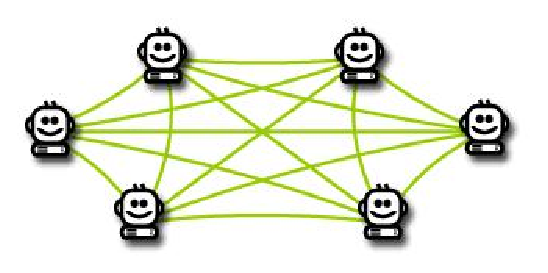
\includegraphics[scale=1]{figs/p2p}

\end{frame}


%%%%%%%%% SLIDE %%%%%%%%%%%%%%%%
\begin{frame}
\frametitle{Outline}
%\tableofcontents[pausesections]
\tableofcontents[]
\end{frame}

\section{Introduction}
\frame<beamer>{\tableofcontents[current]}

%%%%%%%%% SLIDE %%%%%%%%%%%%%%%%
\begin{frame}
\frametitle{Background}
\begin{itemize}
\item Many P2P applications are widely used.
\item Gnutella, Bittorrent, and Skype are developed from the scratch.
\item No P2P abstraction or framework exist.
\item P2P has not made a very large impact in system design.
\end{itemize}
\end{frame}
%%%%%%%%% SLIDE %%%%%%%%%%%%%%%%
\begin{frame}
\frametitle{Building client-server model vs. P2P}
\begin{itemize}
\item Client-server based applications
\begin{itemize}
\item Berkeley sockets library
\item Web frameworks: Java, Python-based Django, Ruby-based Rails
\end{itemize}
\item P2P based applications
\begin{itemize}
\item No such framework or abstraction.
\item Developers must start from nothing to build each application. 
\end{itemize}
\end{itemize}
\end{frame}
%%%%%%%%% SLIDE %%%%%%%%%%%%%%%%
\begin{frame}
\frametitle{Research Overview}
\begin{itemize}
\item Major components to enable wide-scale adoption of P2P by system designers
\begin{enumerate}
\item Scalable and flexible search
\item Efficient network size estimation
\item Reusable search technique on real system
\item Flexible search for P2P DB
\end{enumerate}
\end{itemize}
\end{frame}

%%%%%%%%% SLIDE %%%%%%%%%%%%%%%%
\begin{frame}
\frametitle{Problems}
\begin{itemize}
\item<1-> Efficient Unstructured Search
\begin{itemize}
\item Be optimal in terms of trade-off in query and cache costs
\item Minimize developing and deploying new P2P software(use existing P2P topologies)
\end{itemize}
\item<2-> Network Size Estimation
\begin{itemize}
\item Hard to maintain global network information in P2P systems
\item More accurate but less cost estimation is always preferred. 
\end{itemize}
\item<3-> Reusable Search On Real System
\begin{itemize}
\item Build distributed memory suitable to the P2P network
\item Reference-based datastructure on top of self-managing P2P substrate. e.g. linked list, queue
\item Access control: multiple users, distributed data
\item<4-> Search for P2P DB
\item
\item
\end{itemize}
\end{itemize}
\end{frame}

\iffalse
%\subsection{Search In P2P Networks}
%\frame<beamer>{\tableofcontents[current]}
%%%%%%%%% SLIDE %%%%%%%%%%%%%%%%
\begin{frame}
\frametitle{Search In P2P Networks}
\begin{itemize}
\item Search in unstructured P2P networks
\begin{itemize}
\item Flexible search, such as regular expression search, range queries
\item Requires high communication cost
\end{itemize} 
\item Search in structured P2P networks
\begin{itemize}
\item More efficient
\item Hard to map search matrix to DHT structure
\end{itemize}
\end{itemize}
\end{frame}
%%%%%%%%% SLIDE %%%%%%%%%%%%%%%%
\begin{frame}
\frametitle{Search In P2P Networks}
\begin{itemize}
\item Problem1: Be optimal in terms of trade-off in query and cache costs
\item Problem2: Minimize developing and deploying new P2P software(use existing P2P topologies)
\end{itemize}
\end{frame}
%\subsection{Network Size Estimation}
%\frame<beamer>{\tableofcontents[current]}
%%%%%%%%% SLIDE %%%%%%%%%%%%%%%%
\begin{frame}
\frametitle{Network Size Estimation}
\begin{itemize}
\item Problem1: Hard to maintain global network information in P2P systems
\item Problem2: More accurate but less cost estimation is always preferred. 
\end{itemize}
\end{frame}
%%%%%%%%% SLIDE %%%%%%%%%%%%%%%%
\begin{frame}
\frametitle{Concurrent Datastructure}
\begin{itemize}
\item Problem1: Build distributed memory suitable to the P2P network
\item Problem2: Reference-based datastructure on top of self-managing P2P substrate (list, queue)
\item Problem3: Access control (multiple users, distributed data)
\end{itemize}
\end{frame}
\fi
%\subsection{Concurrent Data Structure}
%\frame<beamer>{\tableofcontents[current]}
\section{Network Size Estimation}
\frame<beamer>{\tableofcontents[current]}

%%%%%%%%% SLIDE %%%%%%%%%%%%%%%%
\begin{frame}
\frametitle{Problem Statement}
\begin{itemize}
\item How many people in this room?
\item Why do you think that?
\singlespacing
\item How many people in this campus?
\item Can you count them all?
\singlespacing
\item How many nodes in a P2P network?
\item The System Monitoring and obtaining global statistics
become much more complex
\end{itemize}
\end{frame}

  %%%%%%%%% SLIDE %%%%%%%%%%%%%%%%

\begin{frame}
\frametitle{Network size estimation}
\begin{itemize}
\item Network Size
\begin{itemize}
\item Load balancing
\item Restricted broadcasting 
\item Determining network parameters
\end{itemize}
\item Unstructured P2P network: broadcasting
\item Structured P2P network: density of identifiers.
\end{itemize}
\end{frame}

  %%%%%%%%% SLIDE %%%%%%%%%%%%%%%%

\iffalse
\begin{frame}
\frametitle{Assumptions}
\begin{itemize}
\item The nodes are uniformly distributed in address space.
\item 
\end{itemize}
\end{frame}
\fi

%%%%%%%%% SLIDE %%%%%%%%%%%%%%%%
\begin{frame}
\frametitle{Basic Approaches}
\begin{minipage}{7cm}
\begin{itemize}
\item $n_{AB}$: The number of nodes in (A,B]
\item $l_{AB}$: The length between A and B - $address_A \ominus address_B$
\item $D$: Node density - the number of nodes in a given length
\begin{eqnarray*}
D = \frac{n_{AB}}{l_{AB}}
\end{eqnarray*}
\item $L$: The length of address space 
\item $\hat{N} = DL$
\end{itemize}
\end{minipage}
\begin{minipage}{3cm}
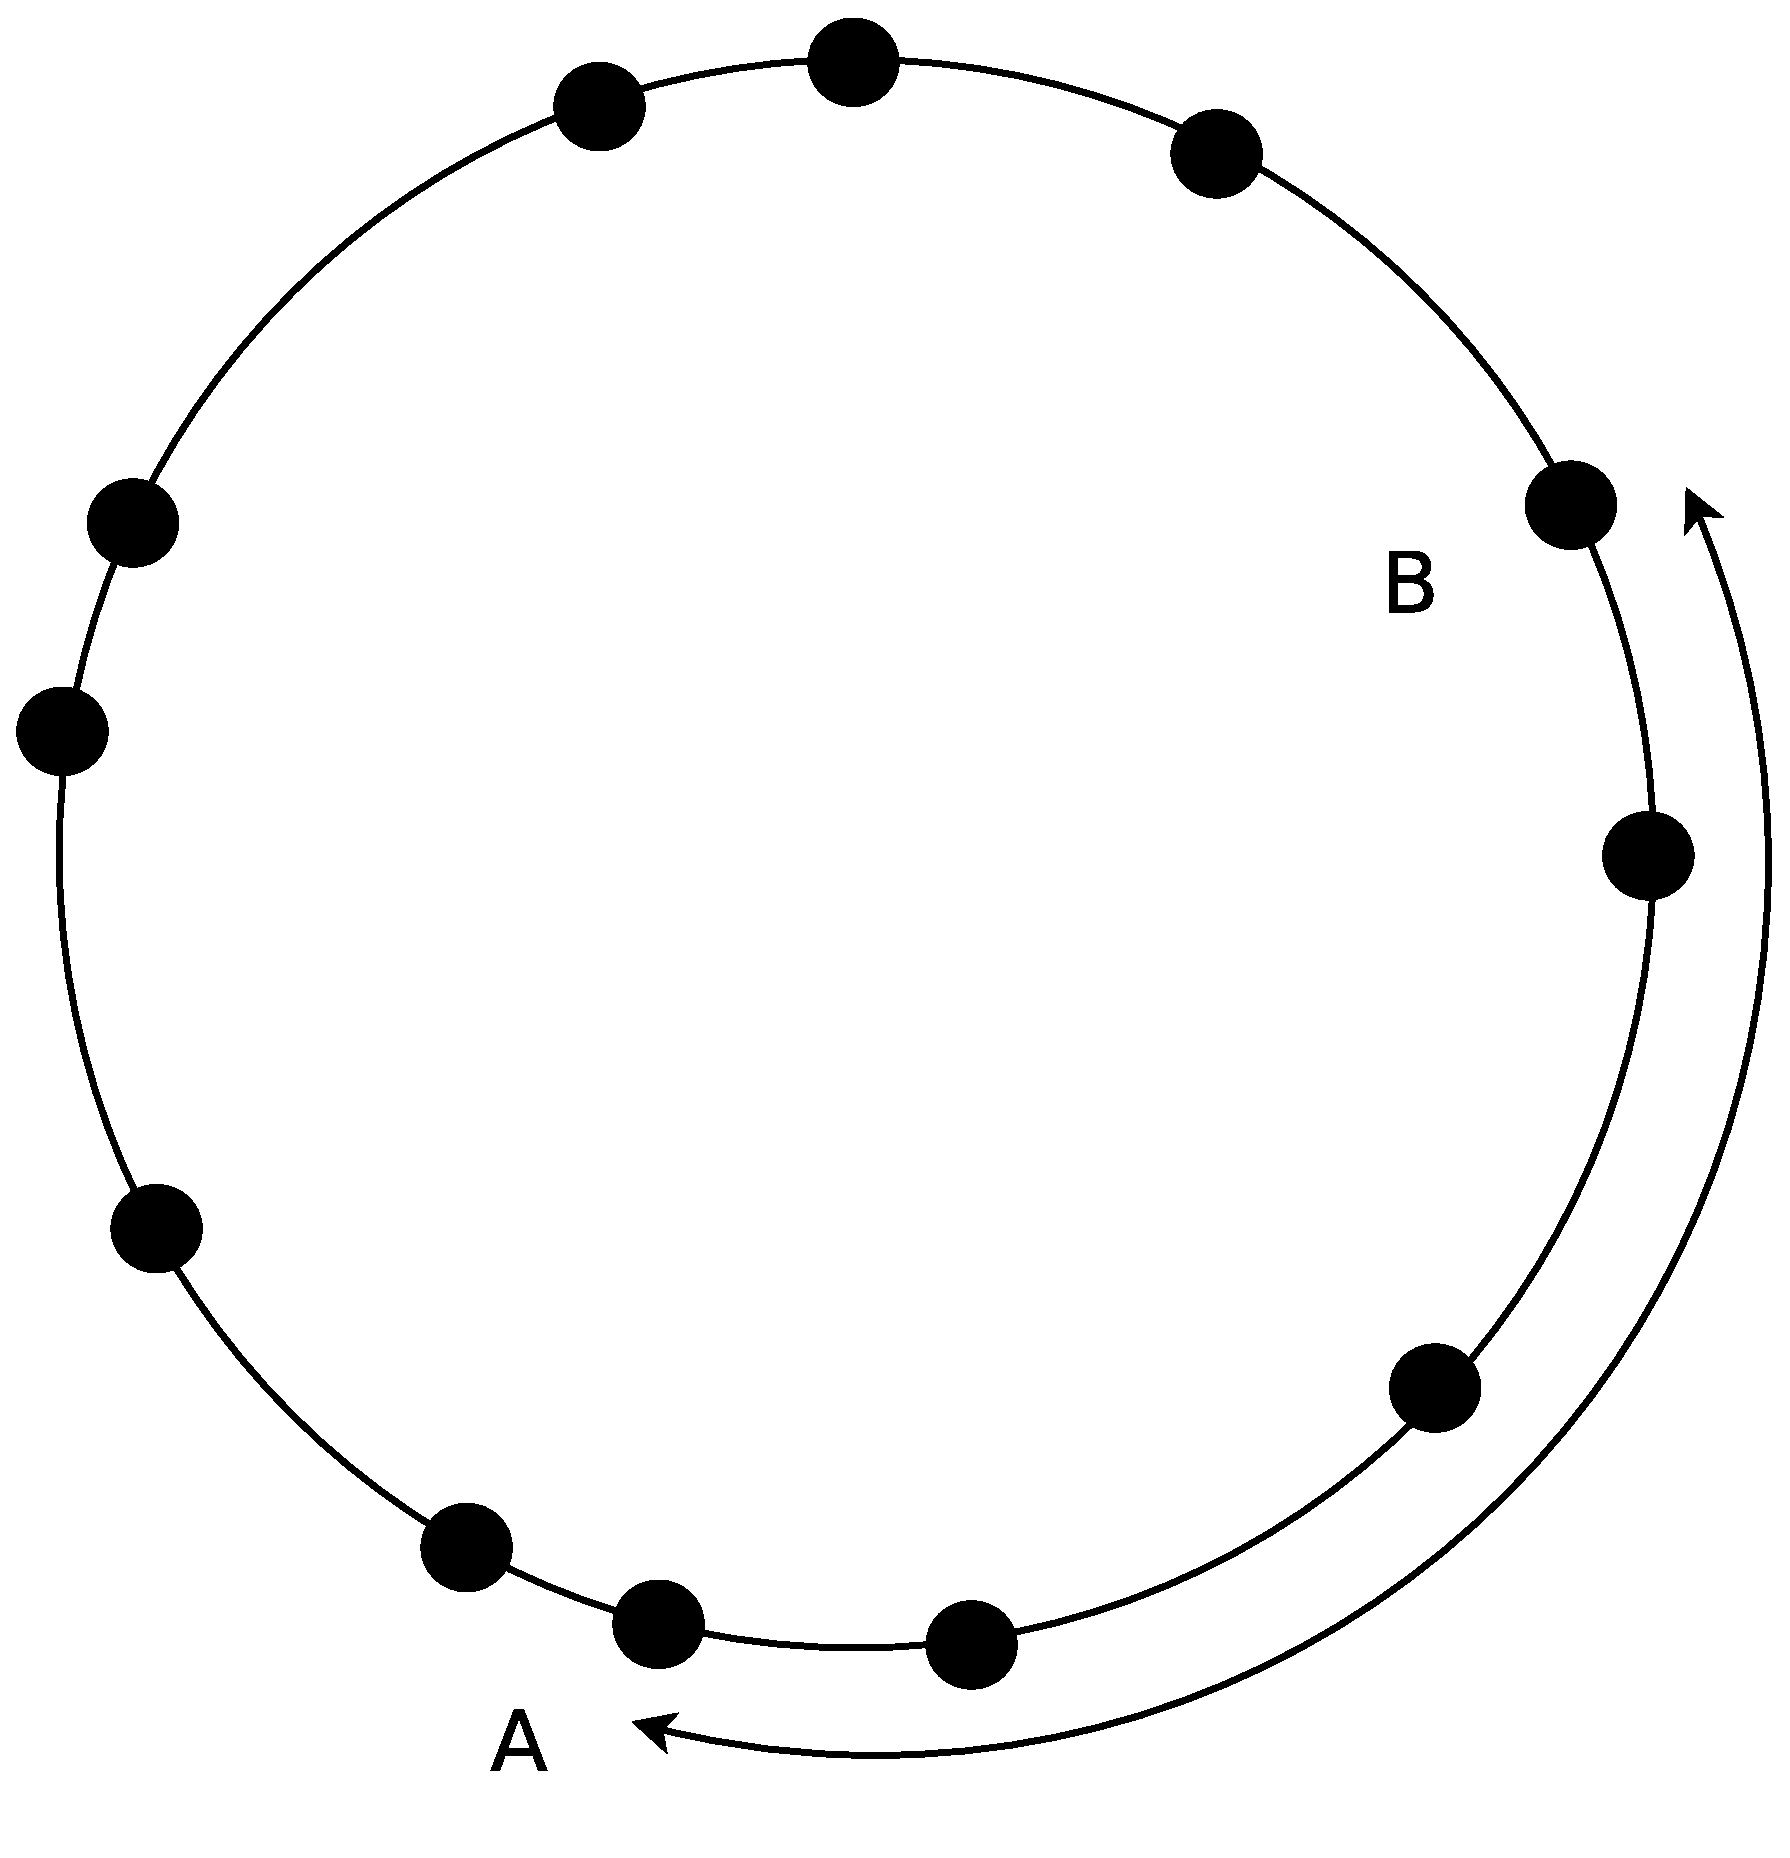
\includegraphics[scale=0.15]{figs/density}
\end{minipage}
\end{frame}
%%%%%%%%% SLIDE %%%%%%%%%%%%%%%%
\begin{frame}
\centering
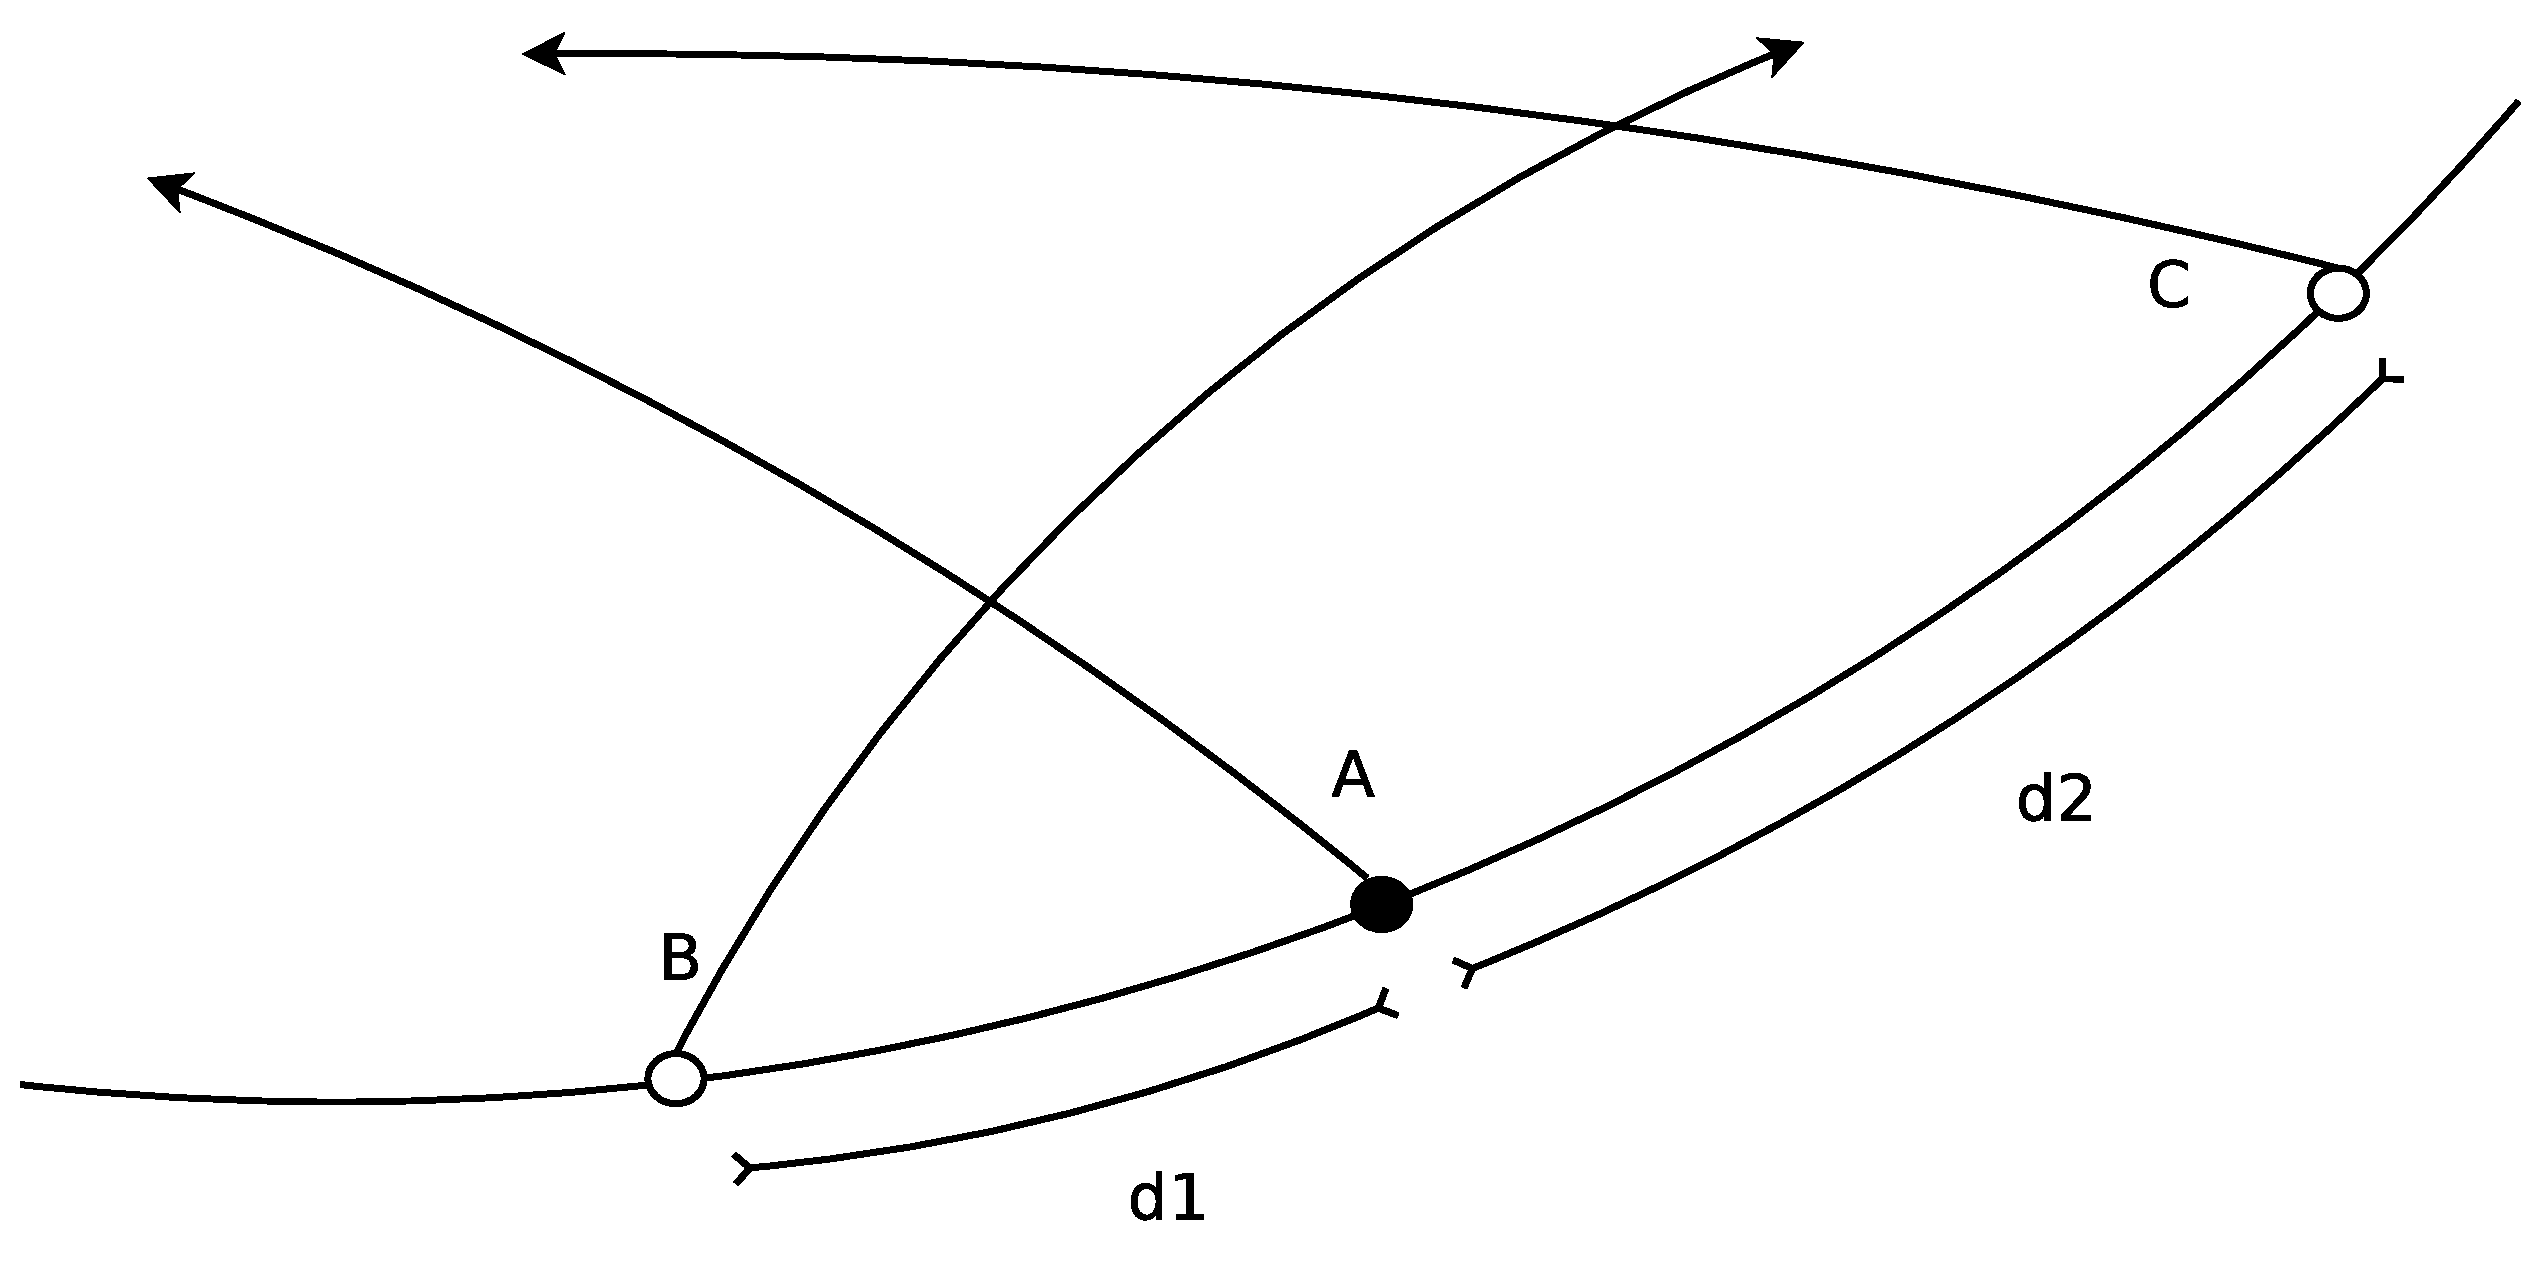
\includegraphics[scale=0.15]{figs/method1}
\frametitle{Method 1: Nearest Estimation}
\begin{itemize}
\item Calculate distances to the nearest neighbors($d_{left}$, $d_{right}$). 
\item $D = \frac{2}{d_{left}+d_{right}}$
\item No communication cost
\end{itemize}
\end{frame}
%%%%%%%%% SLIDE %%%%%%%%%%%%%%%%
\begin{frame}
\frametitle{Method 2: Log Estimation}
\centering
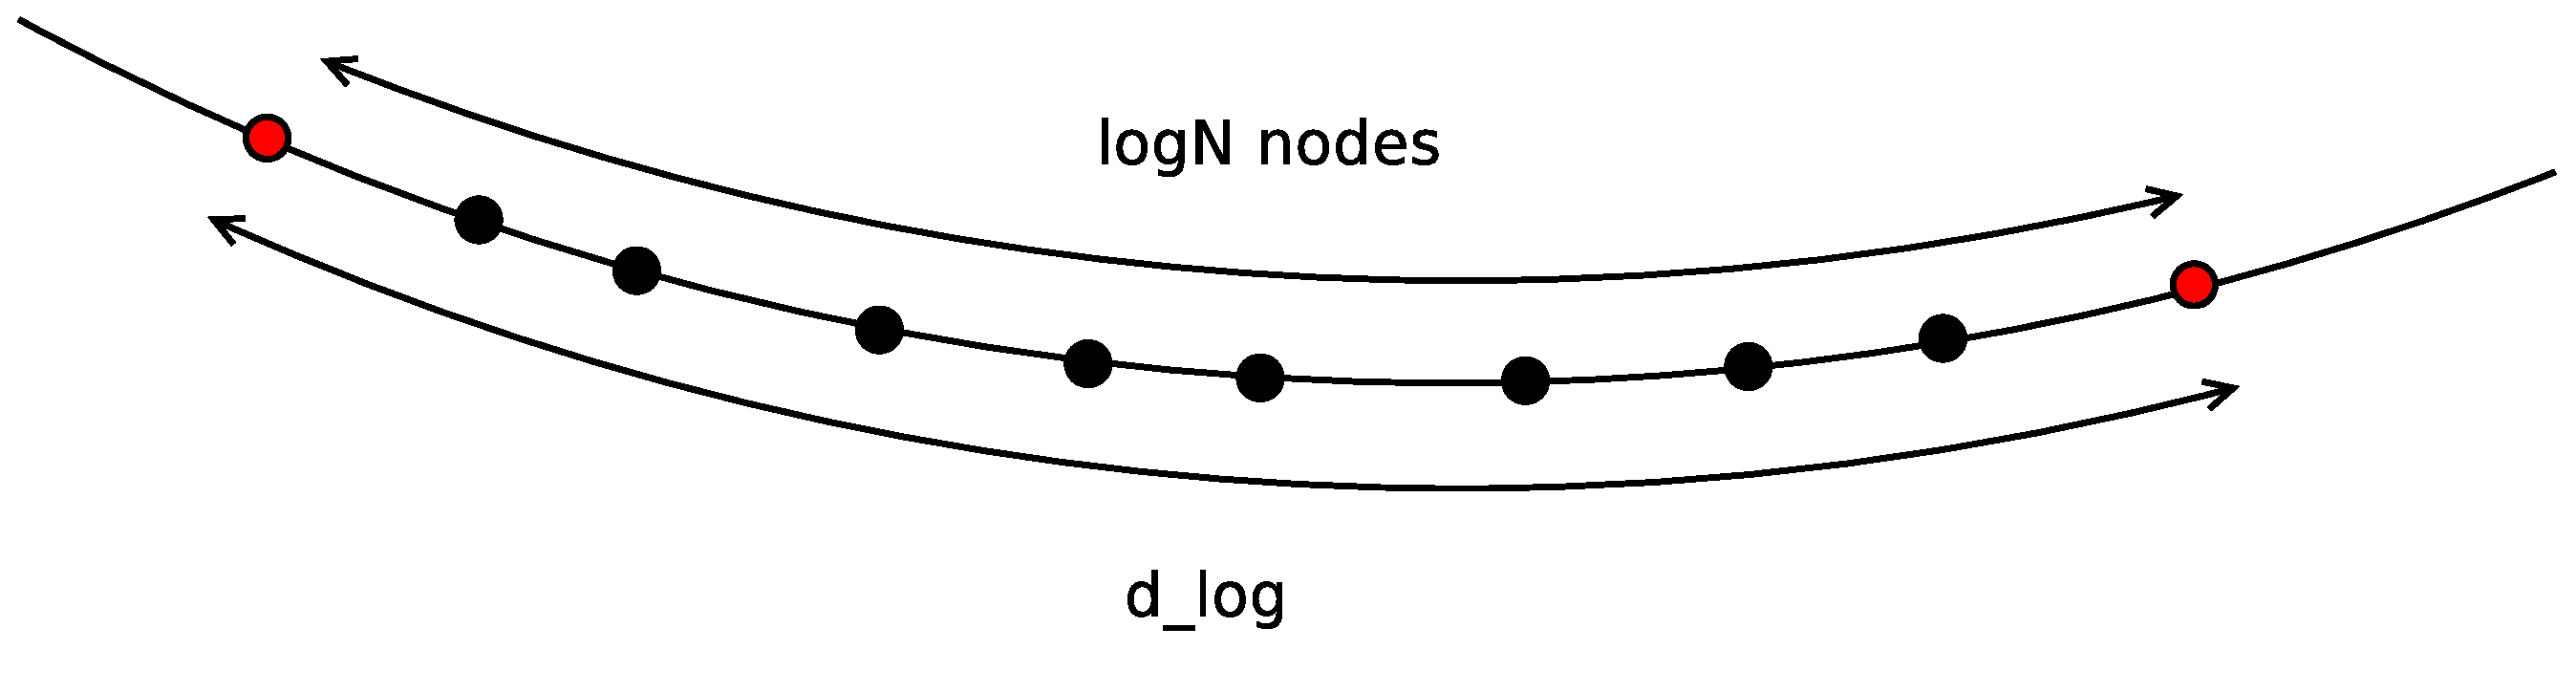
\includegraphics[scale=0.2]{figs/method2}
\begin{itemize}
\item Calculate distance to $\log{N_0}$-hop-away node($d_{log}$).
\item $N_0$ is pre-calculated by the \textbf{nearest estimation}
\item $D = \frac{\log{N_0}}{d_{log}}$
\item $\log{N_0}$ communication cost
\end{itemize}
\end{frame}
%%%%%%%%% SLIDE %%%%%%%%%%%%%%%%
\begin{frame}
\frametitle{Method 3: Median Estimation}
\begin{minipage}{5cm}
\begin{itemize}
\item Take a median from shortcut neighbors' estimation
\item Remote nodes' estimation is the results of \textbf{log estimation} 
\item Communication cost is $deg(n)-2$, where $deg(n)$ is the number of connections of node $n$.
\end{itemize}
\end{minipage}
\begin{minipage}{5cm}
\centering
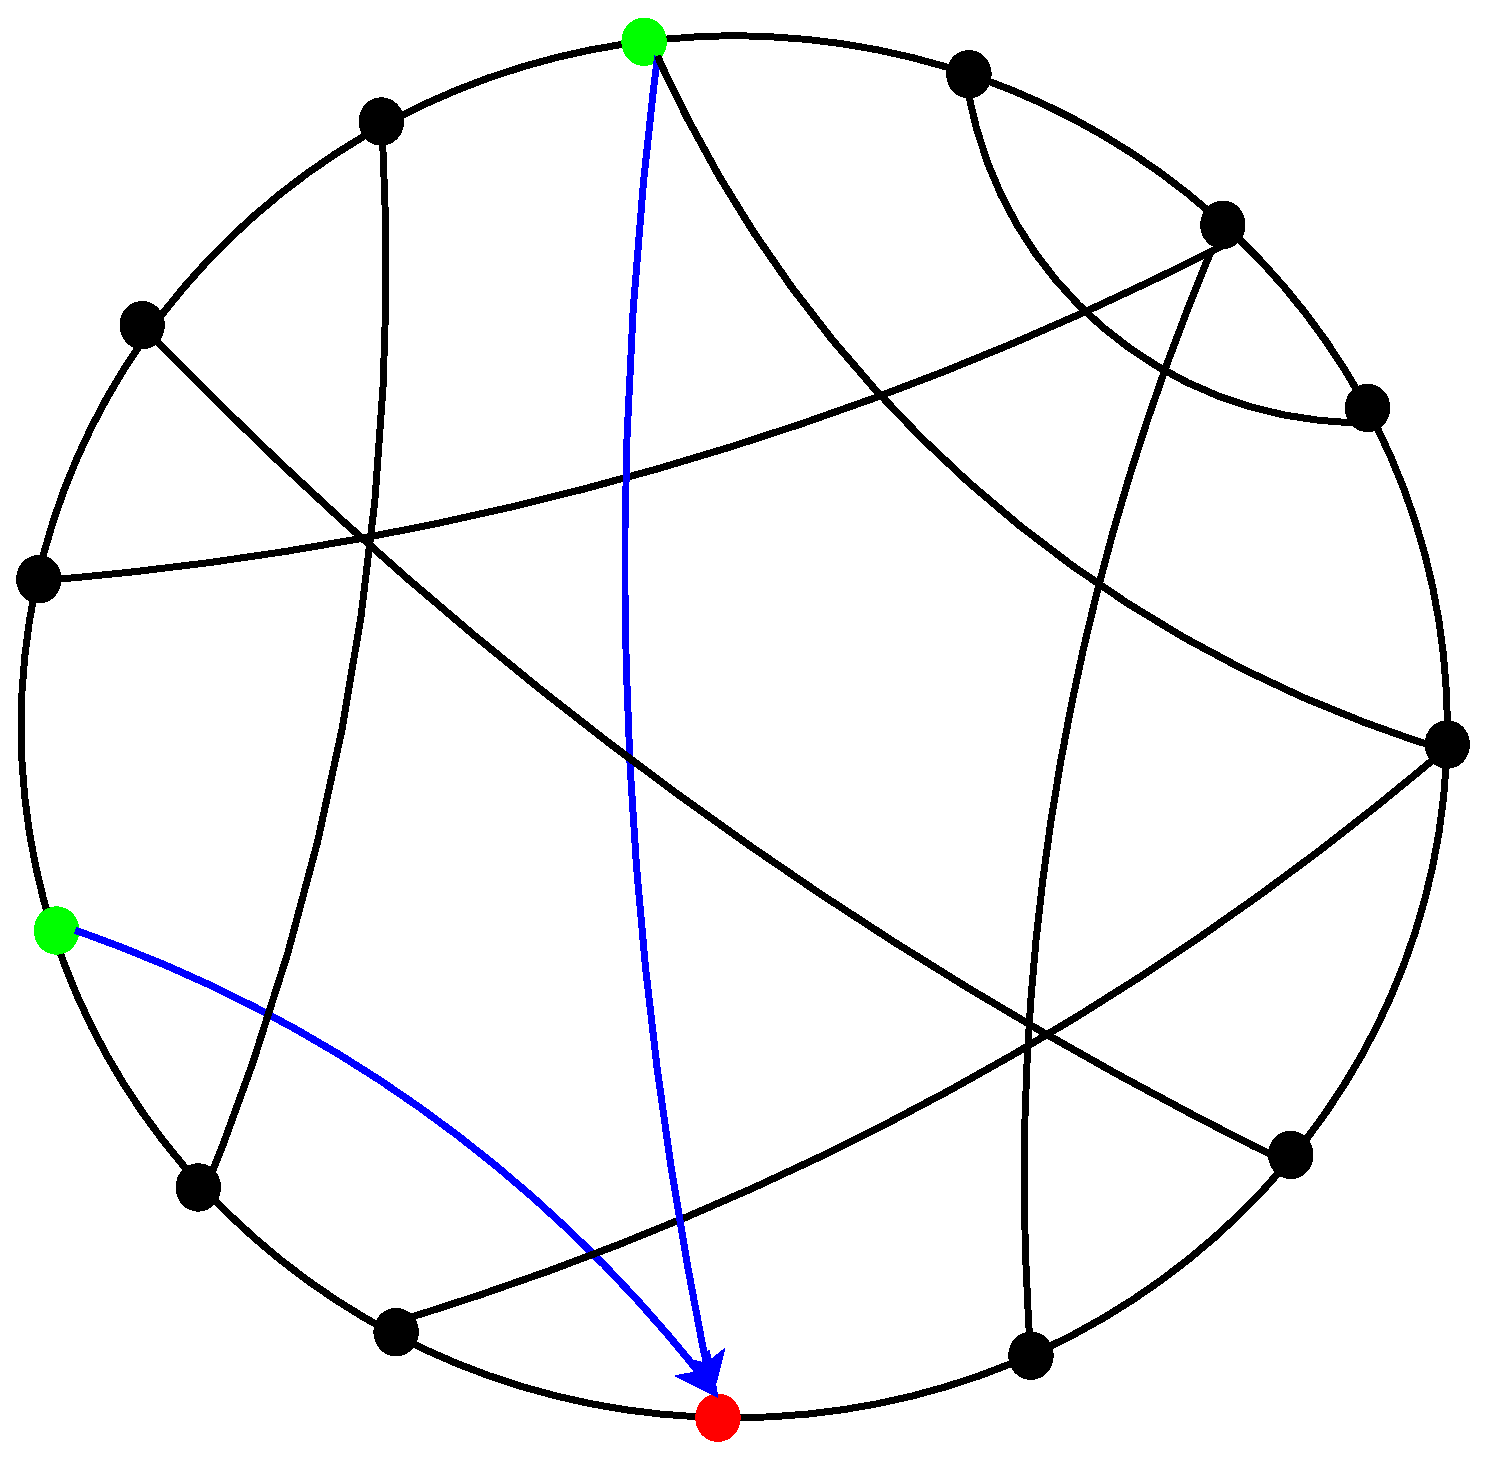
\includegraphics[scale=0.2]{figs/method3}
\end{minipage}
\end{frame}
%%%%%%%%% SLIDE %%%%%%%%%%%%%%%%
\begin{frame}
\frametitle{Method 4: Square-Root Estimation}
\begin{itemize}
\item Use bounded broadcasting
\begin{itemize}
\item Pick a random starting node, $n_{start}$
\item Set a range [$n_{start}$, $n_{start}+\sqrt{N_0}$]
\item Start broadcasting in the range
\item Count the number of nodes in the range
\end{itemize}
\item Broadcasting is bounded by $\sqrt{N_0}$
\item Communication cost is approximately $\sqrt{N_0}$ 
\end{itemize}
\end{frame}
%%%%%%%%% SLIDE %%%%%%%%%%%%%%%%
\begin{frame}
\frametitle{Node Distribution}
\begin{itemize}
\item Nodes in real network are not uniformly distributed. 
\end{itemize}
\begin{figure}
\begin{minipage}{5cm}
\centering
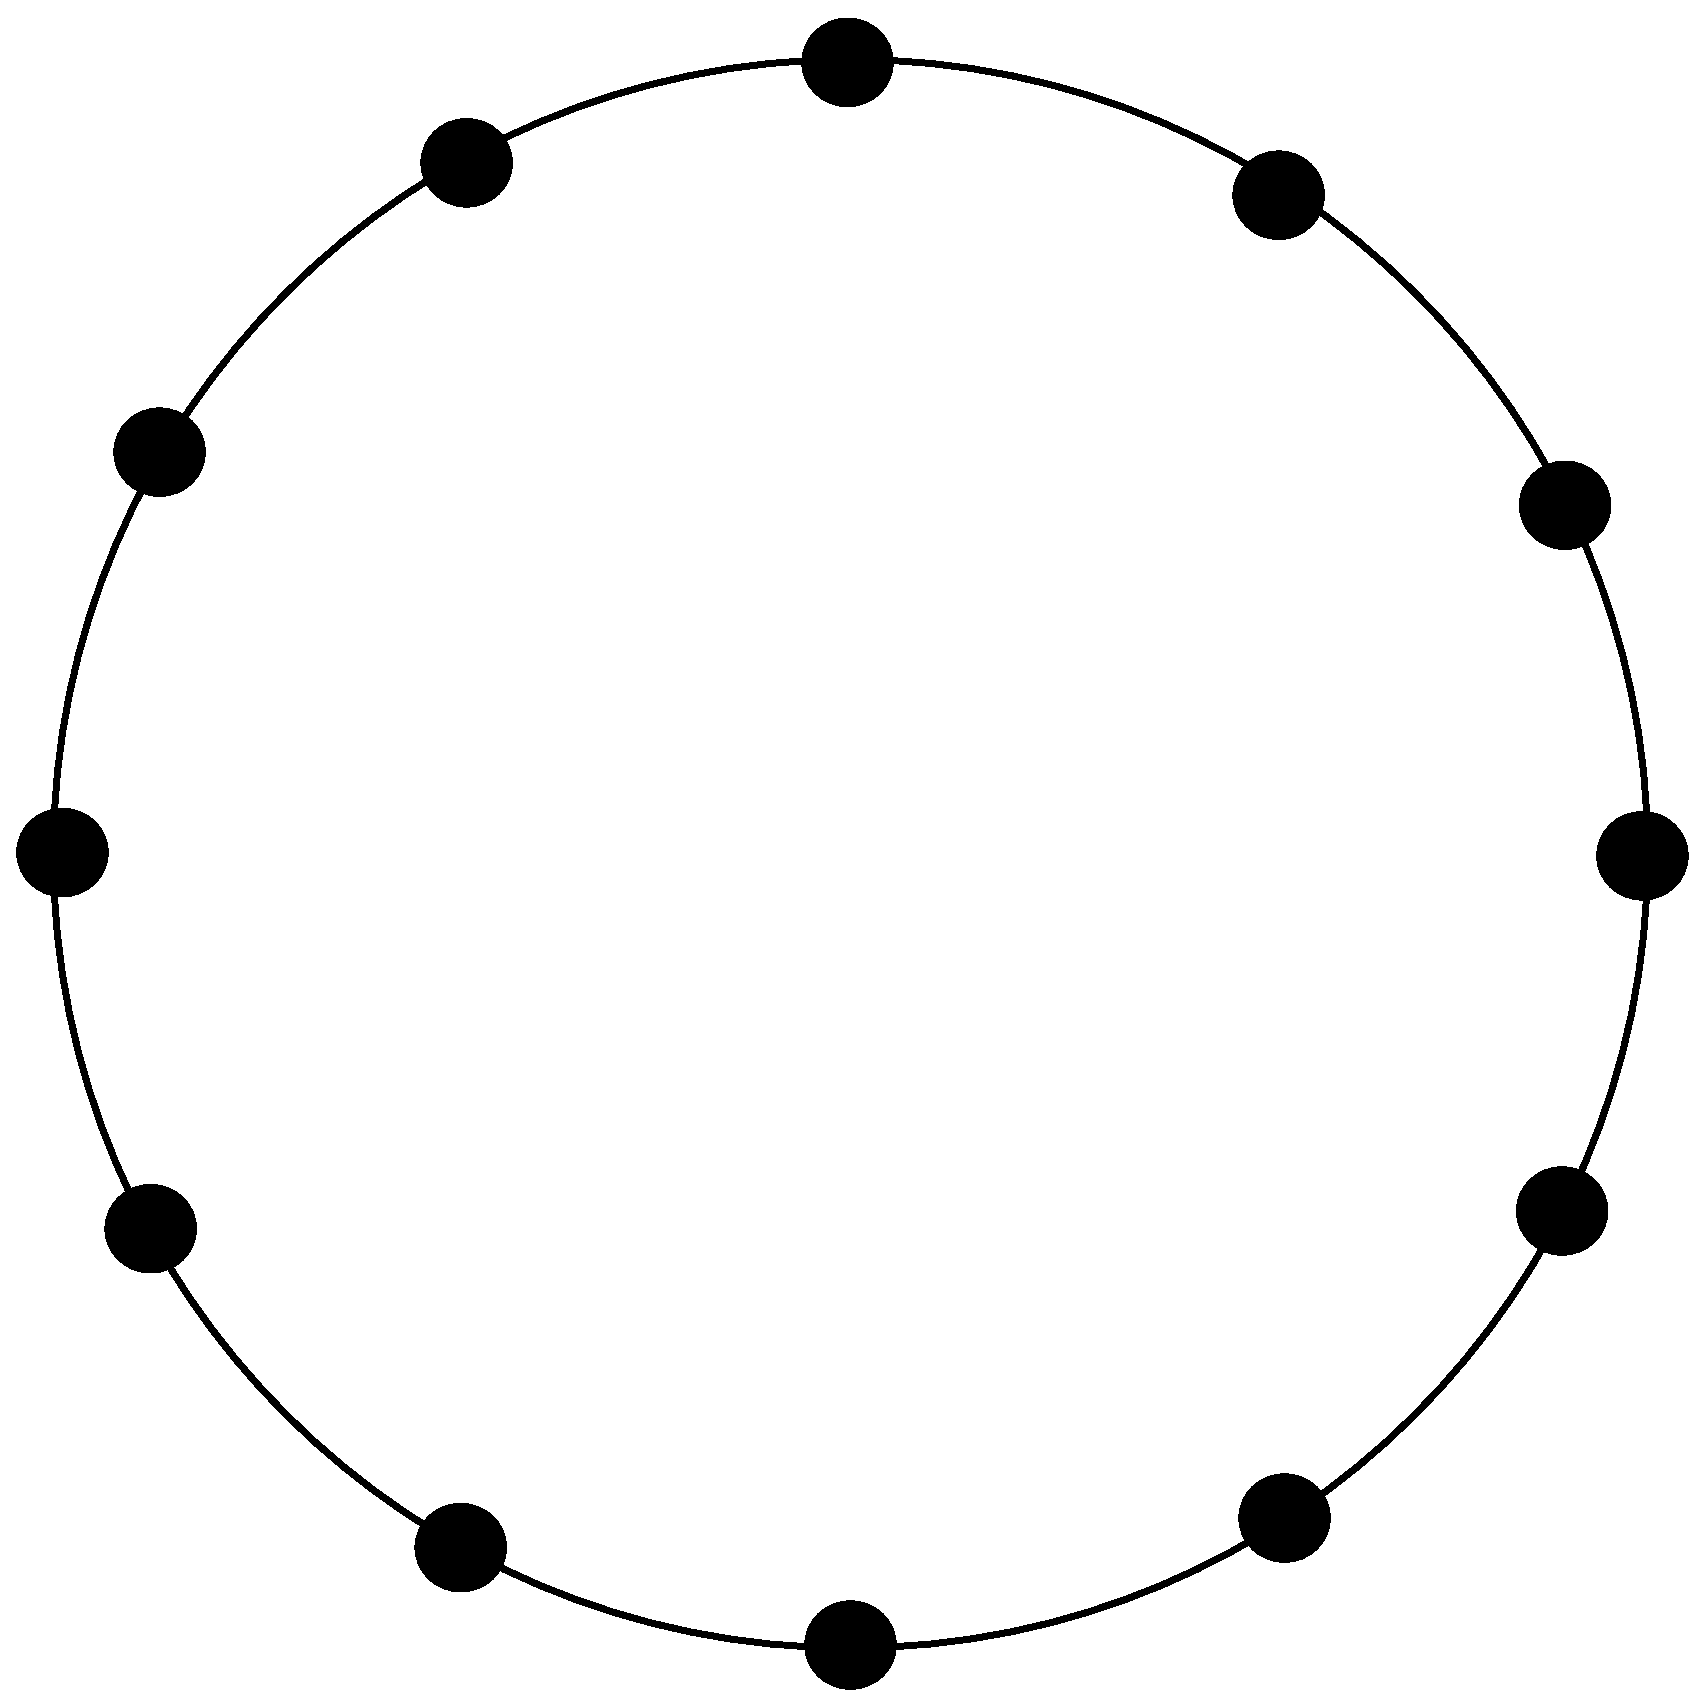
\includegraphics[width=2.0in]{figs/myth}
\caption{Myth} 
\end{minipage}
\begin{minipage}{5cm}
\centering
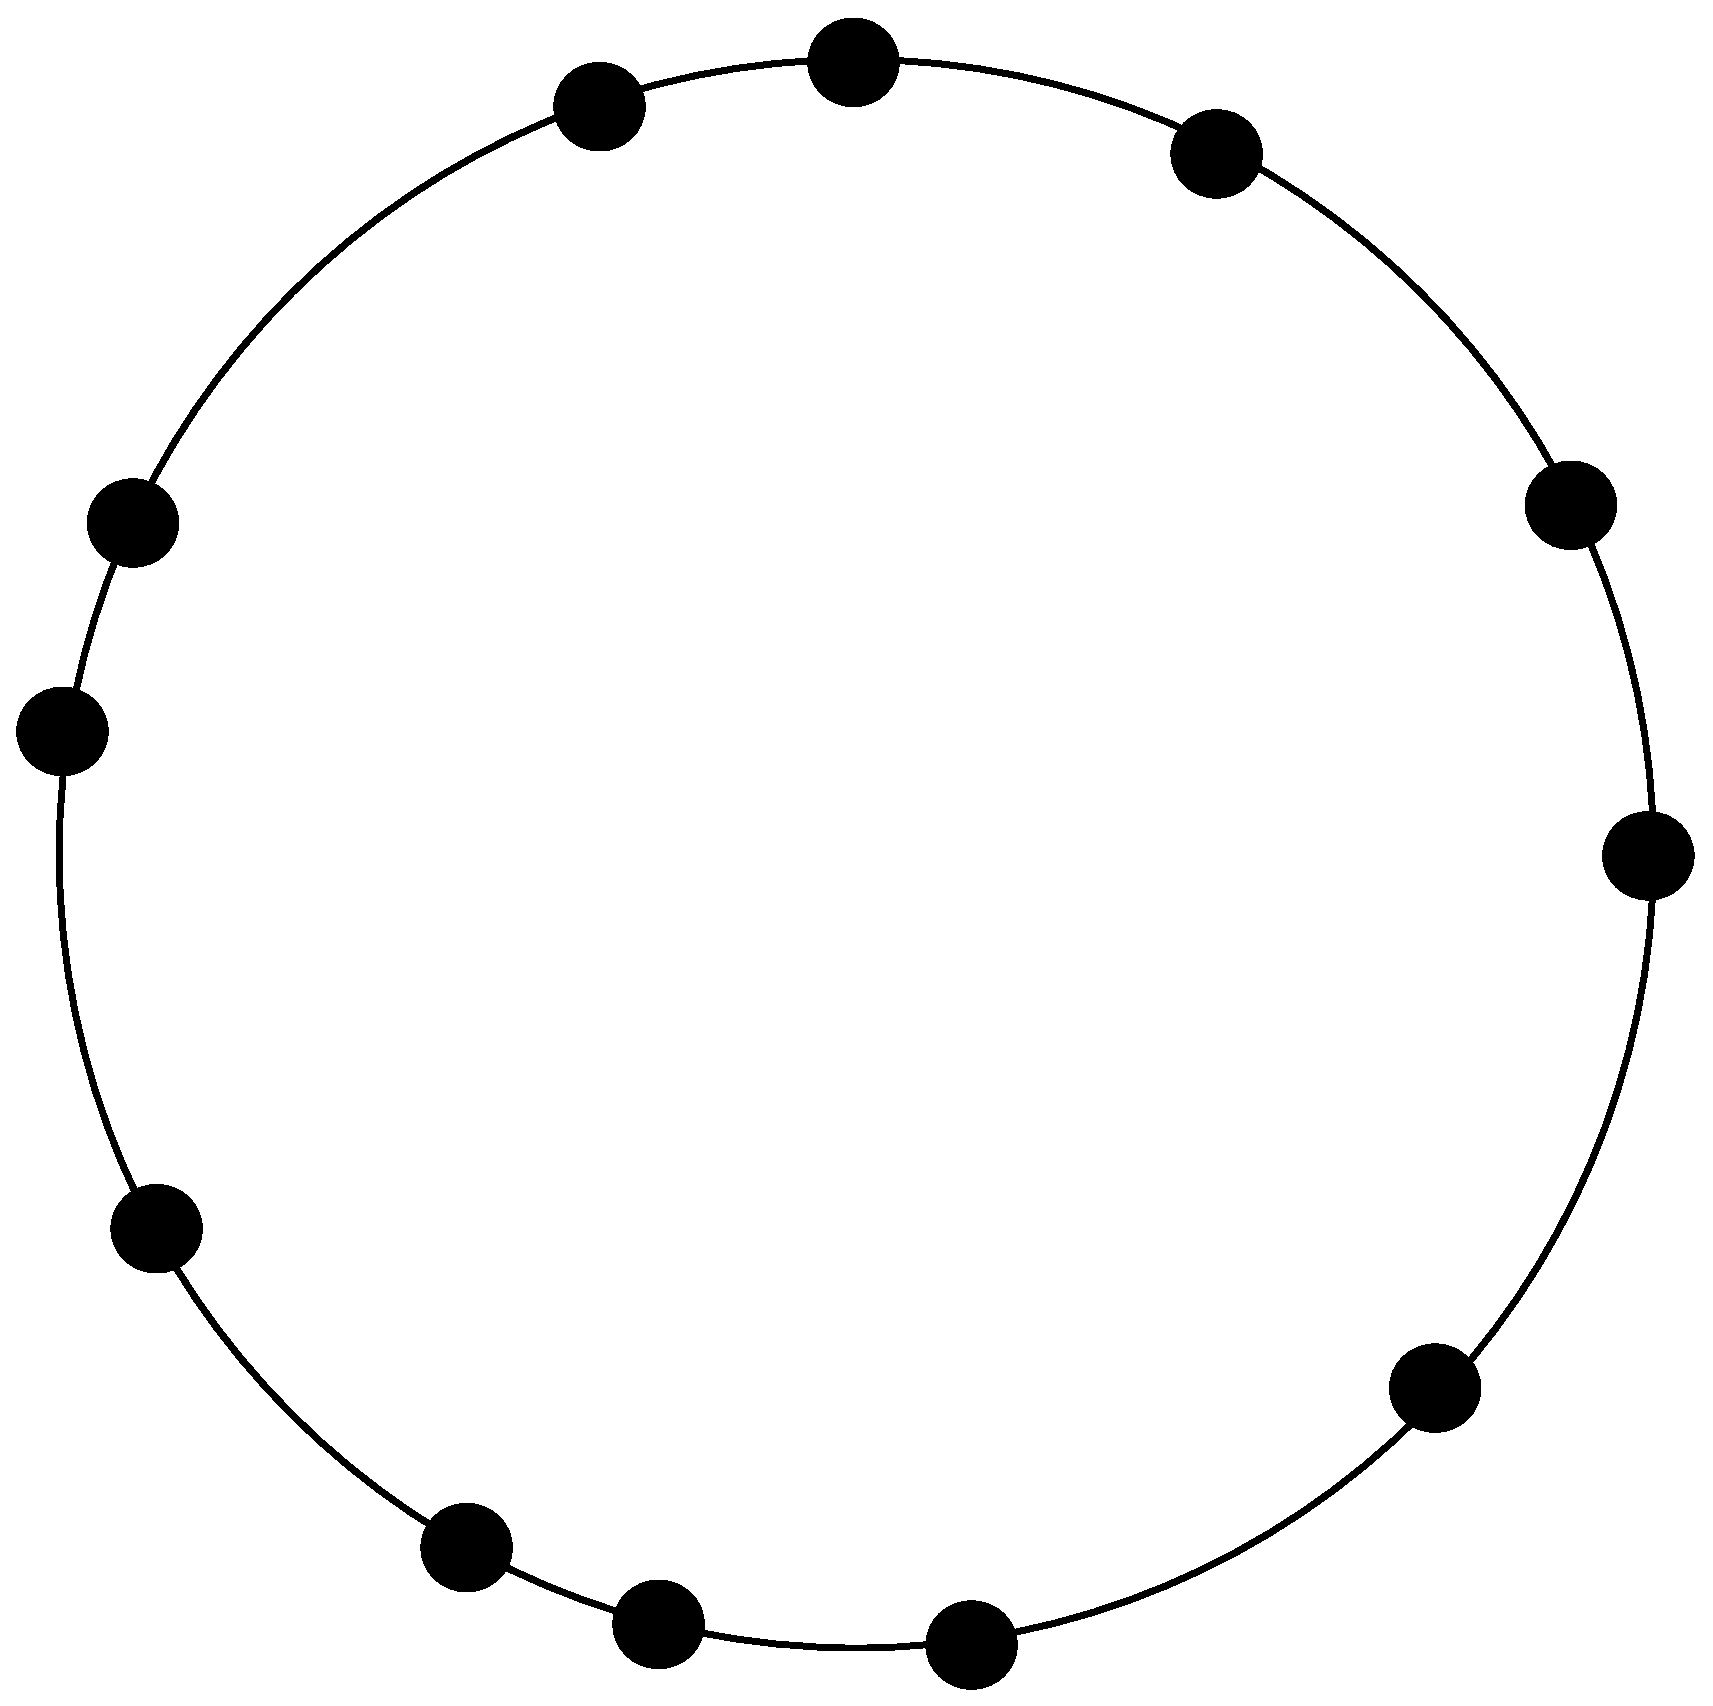
\includegraphics[width=2.0in]{figs/real}
\caption{Real}
\end{minipage}
\end{figure}

\end{frame}
%%%%%%%%% SLIDE %%%%%%%%%%%%%%%%
\begin{frame}
\frametitle{Node Join}
\begin{itemize}
\item Two possible places for join 
\item Select the place with bigger gap between two nodes
\end{itemize}
\center
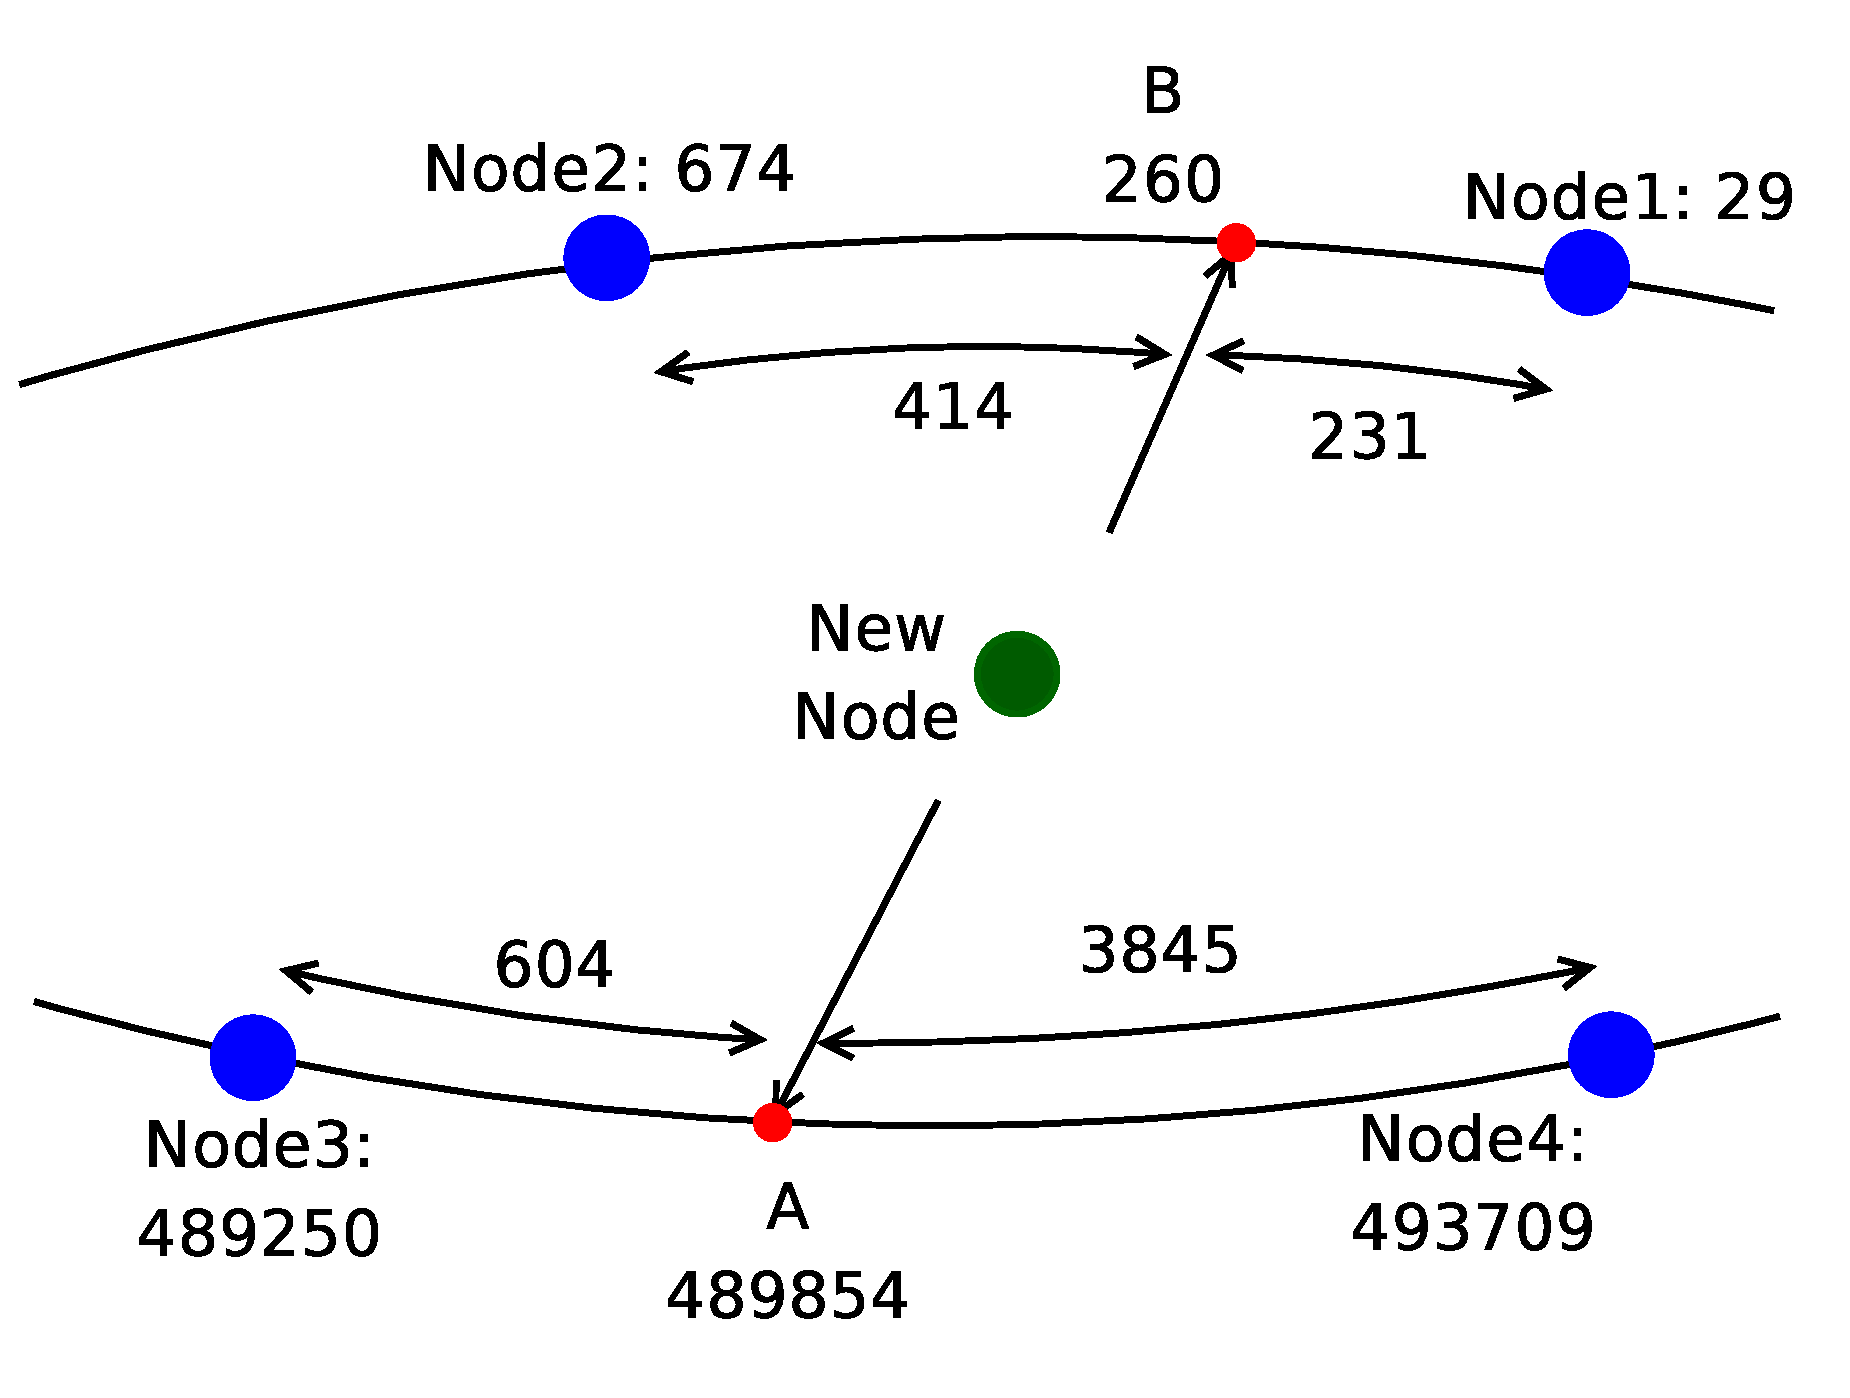
\includegraphics[angle=0,scale=0.2]{figs/evenNet}

\end{frame}
%%%%%%%%% SLIDE %%%%%%%%%%%%%%%%
\begin{frame}
\frametitle{Simulation Result: statistics}
\begin{figure}
\centering
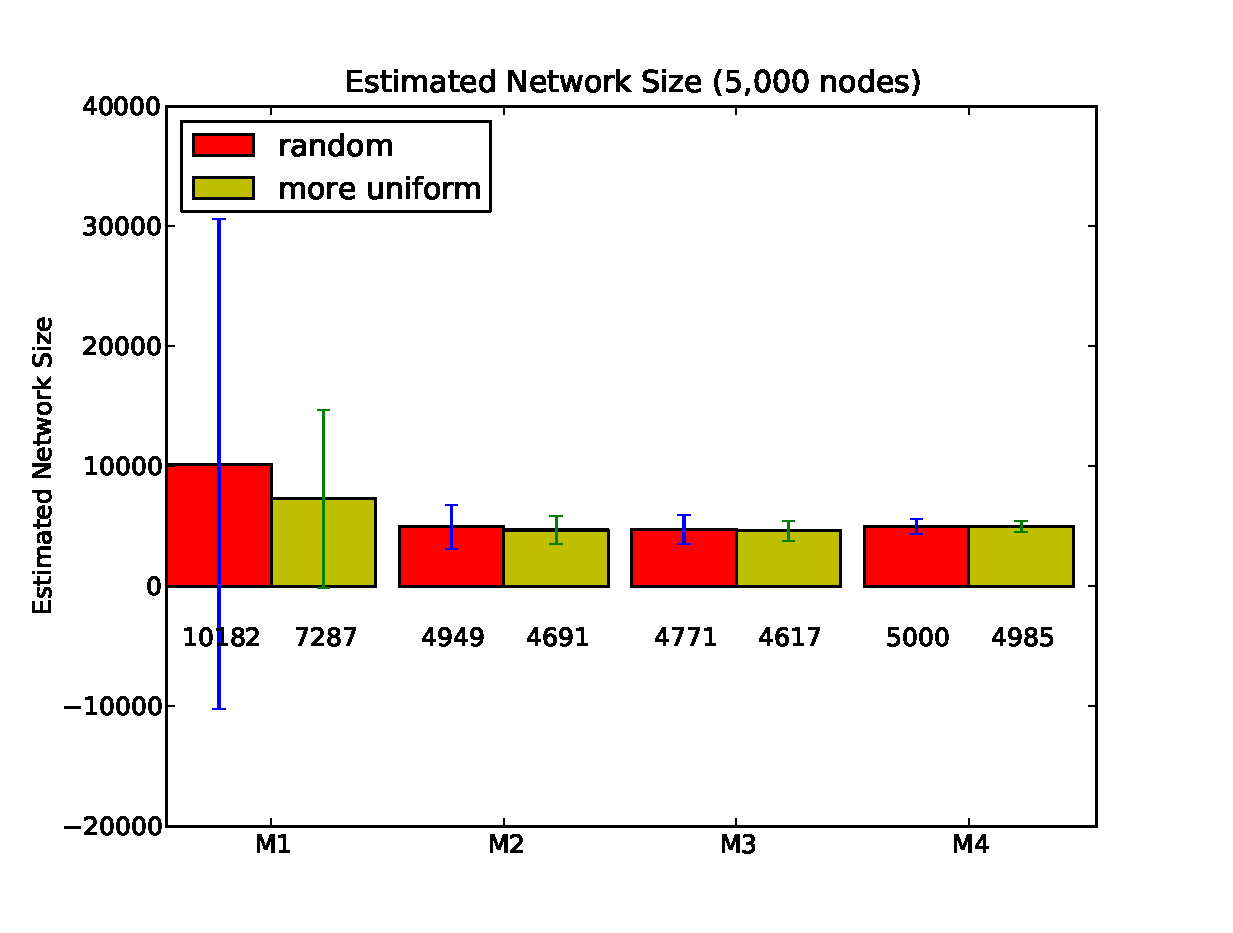
\includegraphics[width=3.5in]{figs/size5k}
\end{figure}
\end{frame}
%%%%%%%%% SLIDE %%%%%%%%%%%%%%%%
\begin{frame}
\frametitle{Simulation Result: statistics}
\begin{figure}
\centering
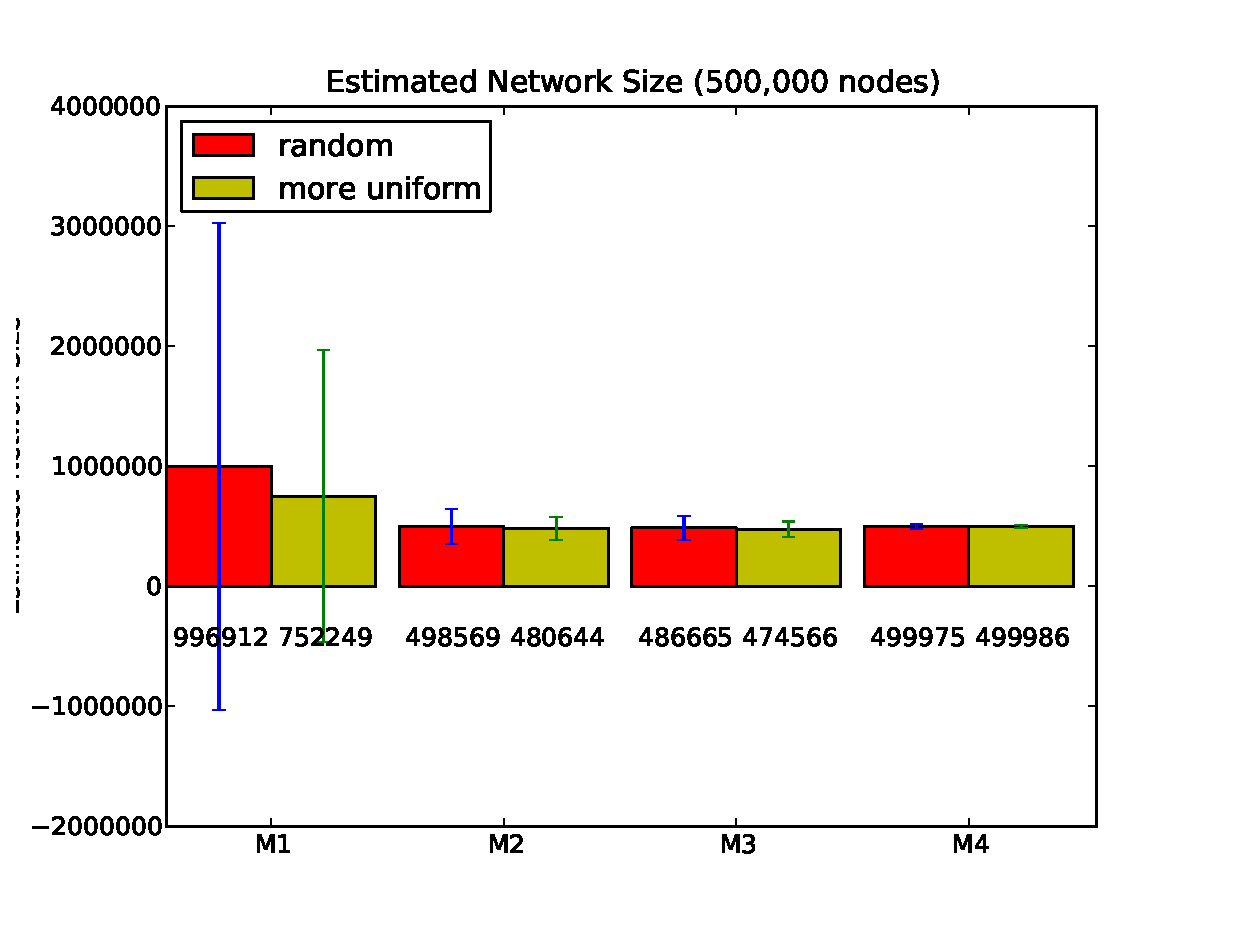
\includegraphics[width=3.5in]{figs/size500k}
\end{figure}
\end{frame}
%%%%%%%%% SLIDE %%%%%%%%%%%%%%%%
\begin{frame}
\frametitle{Simulation Result: Cost}
\begin{figure}
\centering
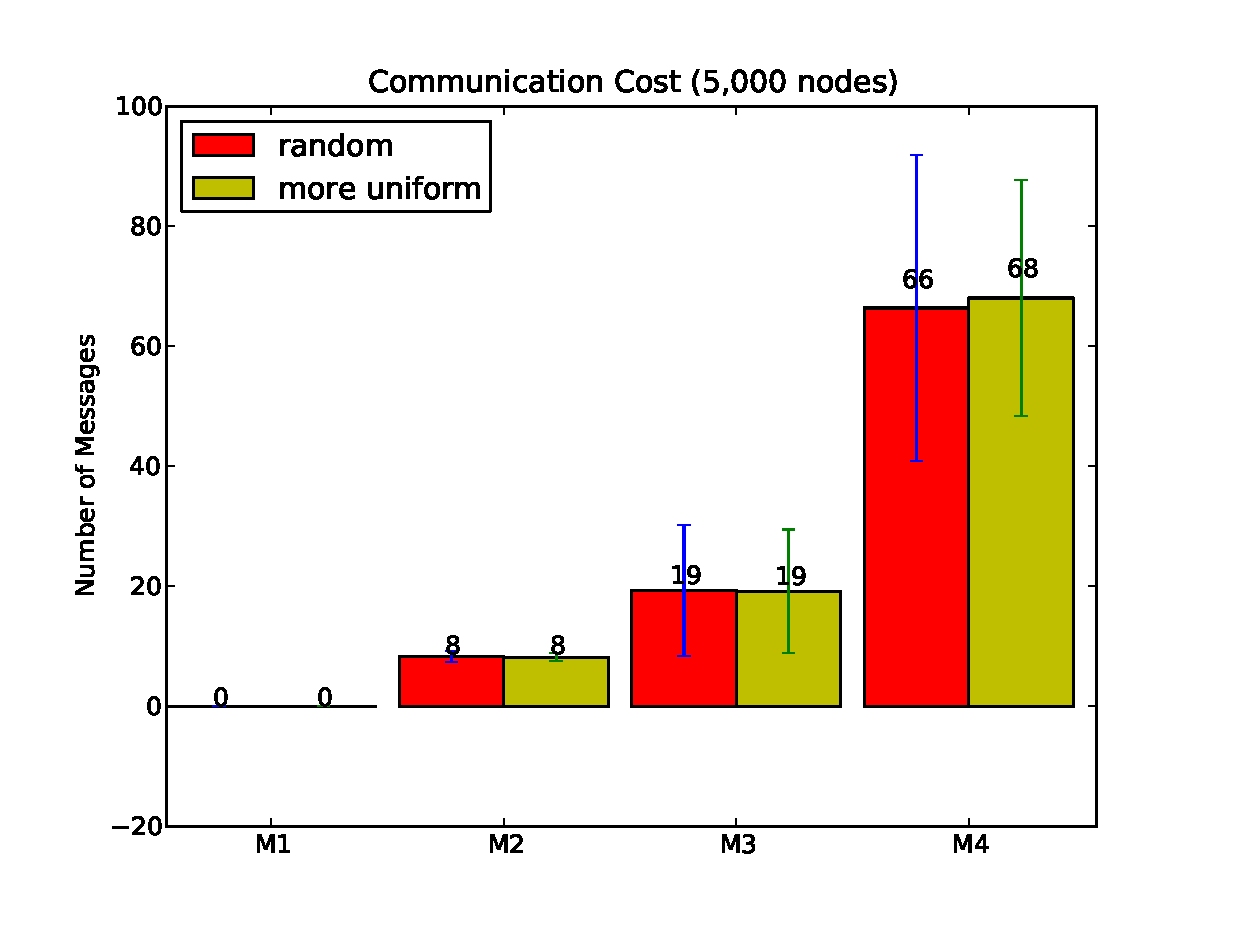
\includegraphics[width=3.5in]{figs/cost5k}
\end{figure}
\end{frame}
%%%%%%%%% SLIDE %%%%%%%%%%%%%%%%
\begin{frame}
\frametitle{Simulation Result: Cost}
\begin{figure}
\centering
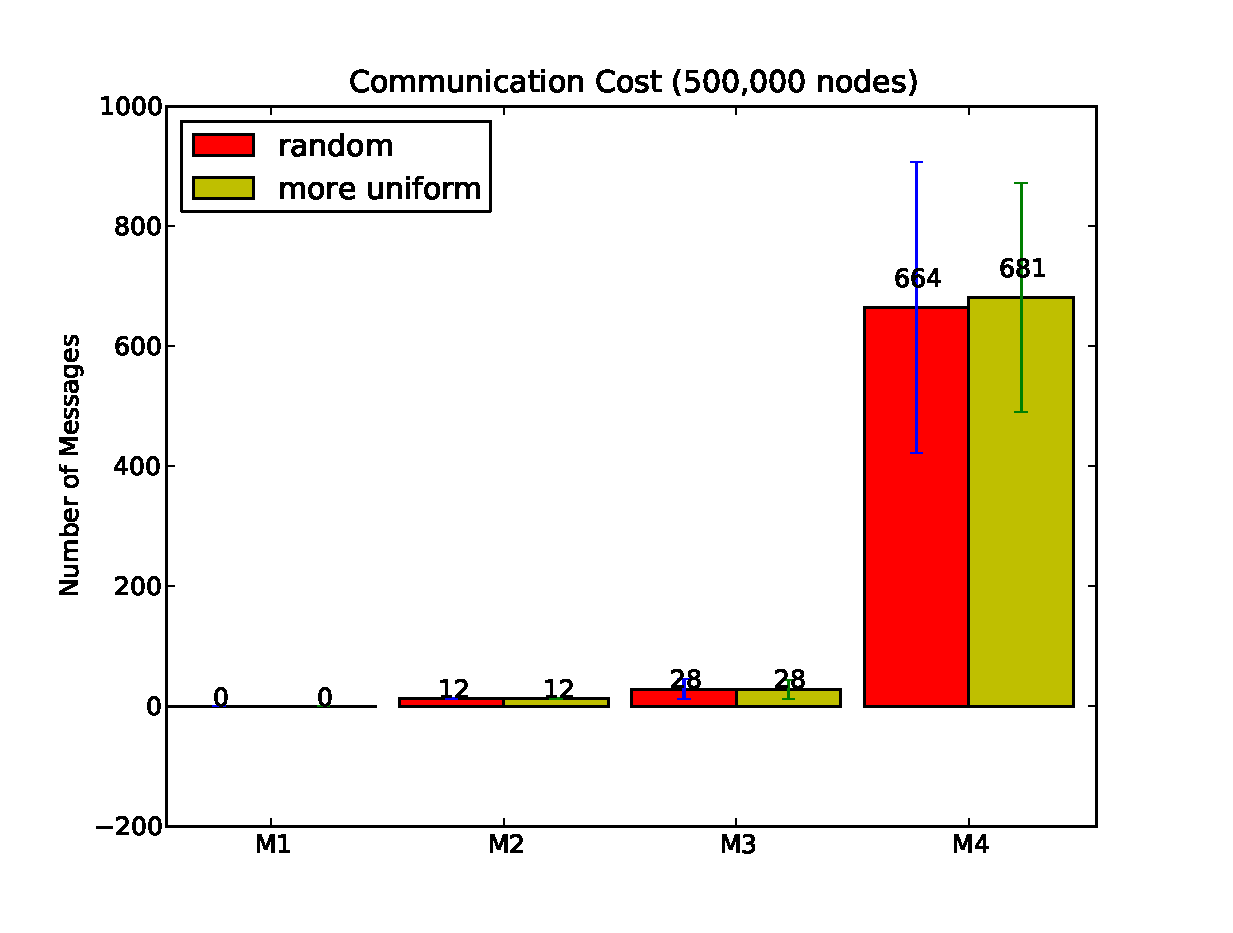
\includegraphics[width=3.5in]{figs/cost500k}
\end{figure}
\end{frame}

%%%%%%%%% SLIDE %%%%%%%%%%%%%%%%
\begin{frame}
\frametitle{Contribution}
\begin{itemize}
\item Each method achieves various accuracy and cost.
\item A user can select one or more combined methods to meet user's desired performance.
\item Introduce node join algorithm to make a network more uniformly distributed.
\end{itemize}
\end{frame}


\section{Deetoo: Search in P2P Networks}
\frame<beamer>{\tableofcontents[current]}



%%%%%%%%% SLIDE %%%%%%%%%%%%%%%%
\begin{frame}
\frametitle{Routing Methods}
\begin{itemize}
%\item<1->
\item
Flooding or Random Walks:
\begin{itemize}
\item Unstructured Networks
\item simple, general query like key-word search
\item message overload ($O(N)$) - scaling problem
\item ex. Gnutella
\end{itemize}
%\item<2->
\item
DHT-based Greedy Routing
\begin{itemize}
\item Overlay topology is Structured
\item Objects at specific location
\item Efficient query resolving and scalable ($O(\log{N})$)
\item Need for complicated indices for routing
\item ex. CAN, Chord
\end{itemize}
\end{itemize}

\end{frame}

%----------------------------------------------------------------------------------
%-------------------Deetoo---------------------------------------------------------

%\section{Basic Idea}
%%%%%%%%% SLIDE %%%%%%%%%%%%%%%%
\begin{frame}
\frametitle{Deetoo: Basic Idea}
\begin{itemize}
%\item<1-> 
\item
Build efficient routable unstructured network.
%\item<2-> 
\item
Support any type of query (key-word search, partial match, or regular expression match)
%\item<3-> 
\item
Use bounded broadcasting in 1-dimensional small world network.
\end{itemize}
\end{frame}

%%%%%%%%% SLIDE %%%%%%%%%%%%%%%%
%\begin{frame}
%\frametitle{Structure}
%\begin{itemize}
%\item<1-> Two virtual rings for caching and querying respectively
%\begin{itemize}
%\item Each ring is 1-dimensional small world network
%\item Each node has an address for cache and translated query address. 
%\end{itemize}
%\item<2-> Unstructured table
%\begin{itemize}
%\item n$\times$ n array
%\item Insert object into each bin in subset of columns.
%\item To search for an object, select random rows and check each bin in those rows for the object.
%\end{itemize}
%\end{itemize}
%%%%%%%%% SLIDE %%%%%%%%%%%%%%%%
\begin{frame}
\frametitle{Caching and query space}

\begin{figure}
\centering
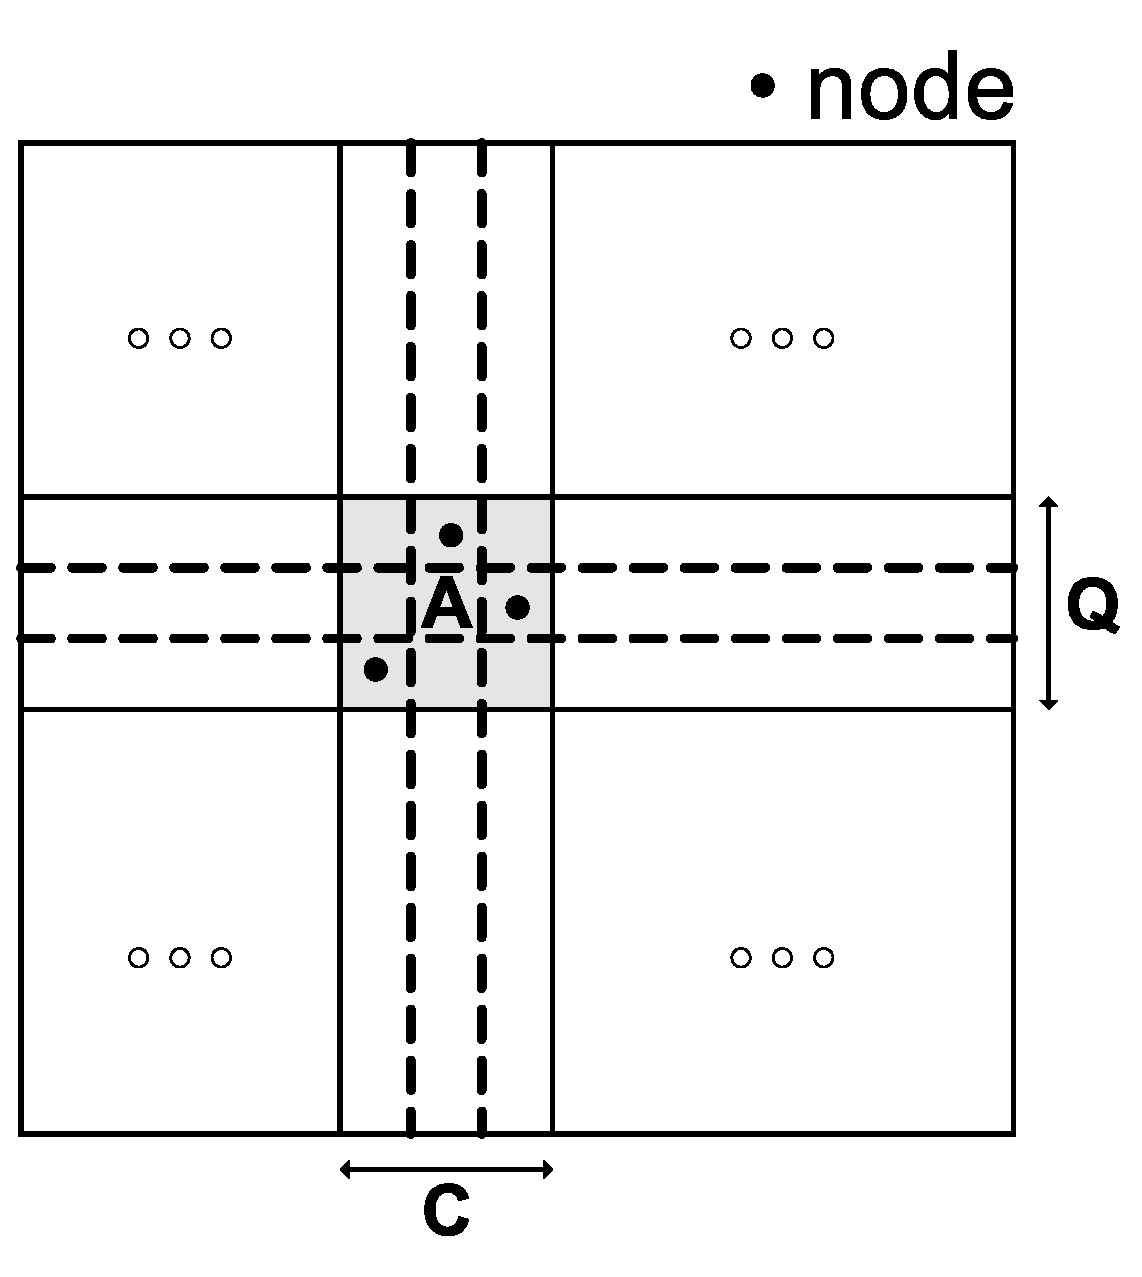
\includegraphics[width=2.5in]{figs/space}
\end{figure}

\end{frame}

%%%%%%%%% SLIDE %%%%%%%%%%%%%%%%
\begin{frame}
\frametitle{Topology}
\begin{figure}
\centering
\begin{tabular}{c|c|c}
\begin{minipage}[t]{1.3in}
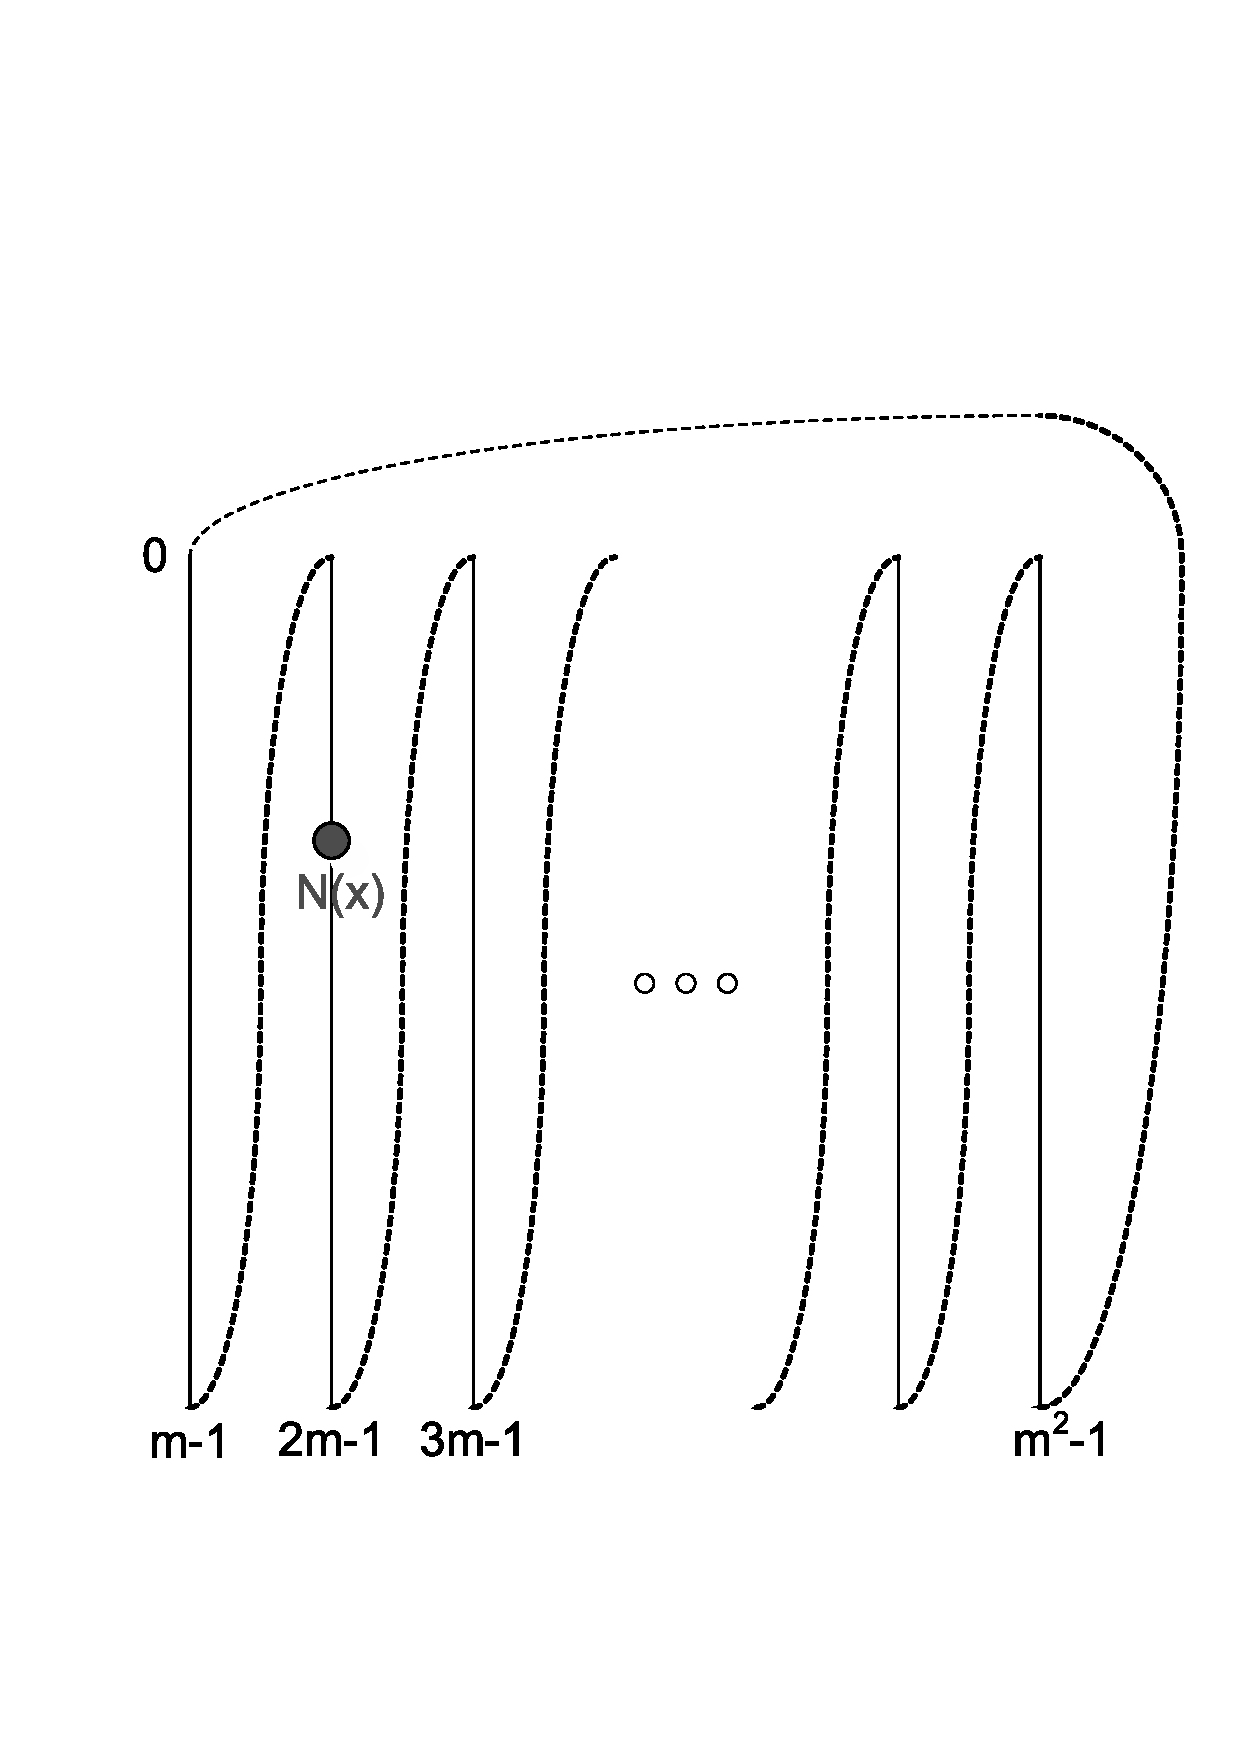
\includegraphics[width=1.2in]{figs/cache}
\caption{Virtual Ring 1 for caching.}
\end{minipage}
& \begin{minipage}[t]{1.3in}
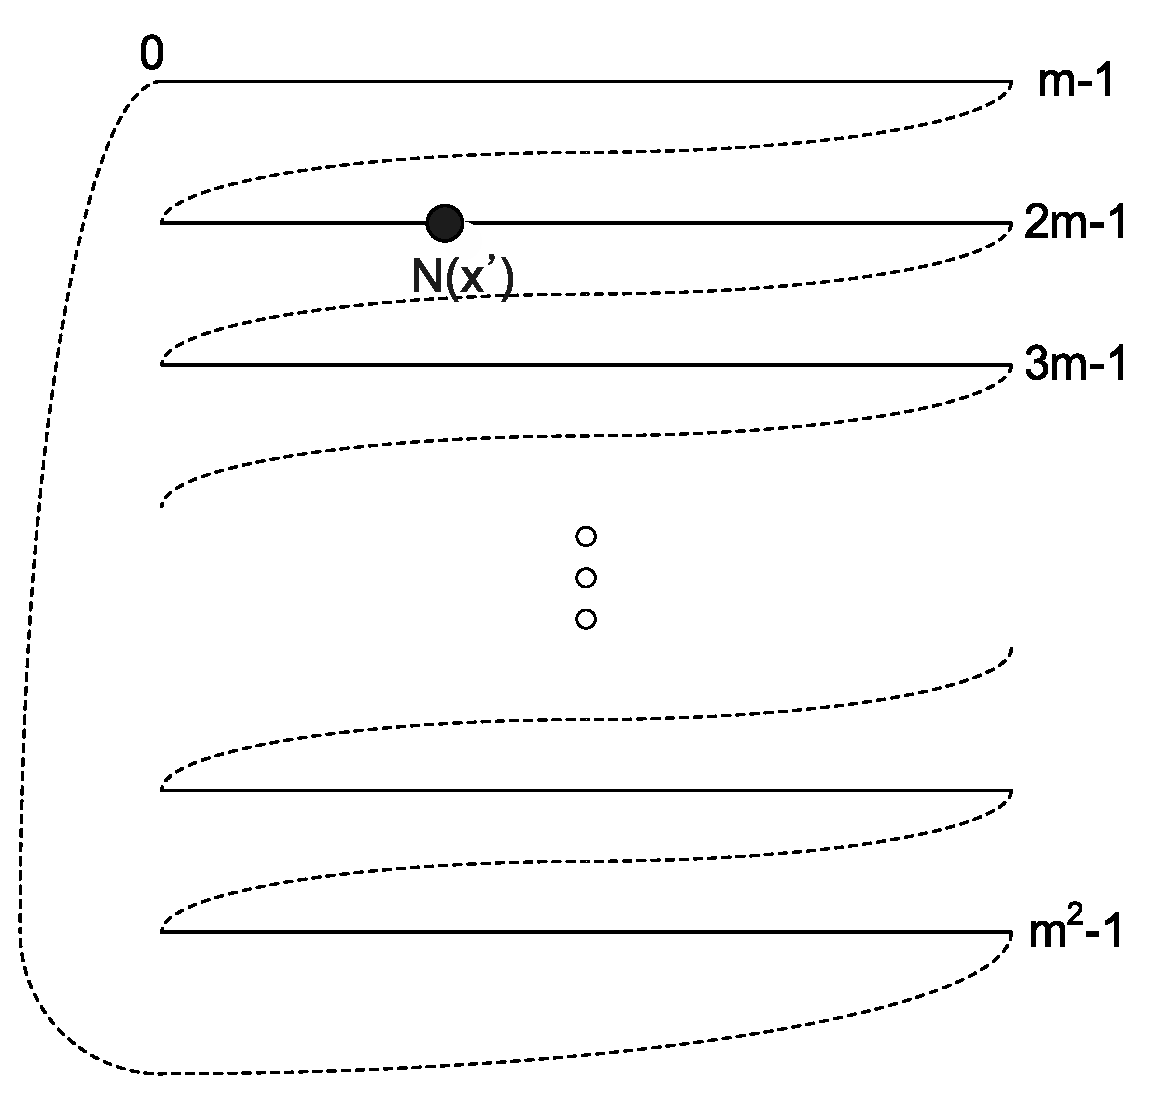
\includegraphics[width=1.2in]{figs/query}
\caption{Virtual Ring 2 for Queries.}
\end{minipage}
& \begin{minipage}[t]{1.3in}
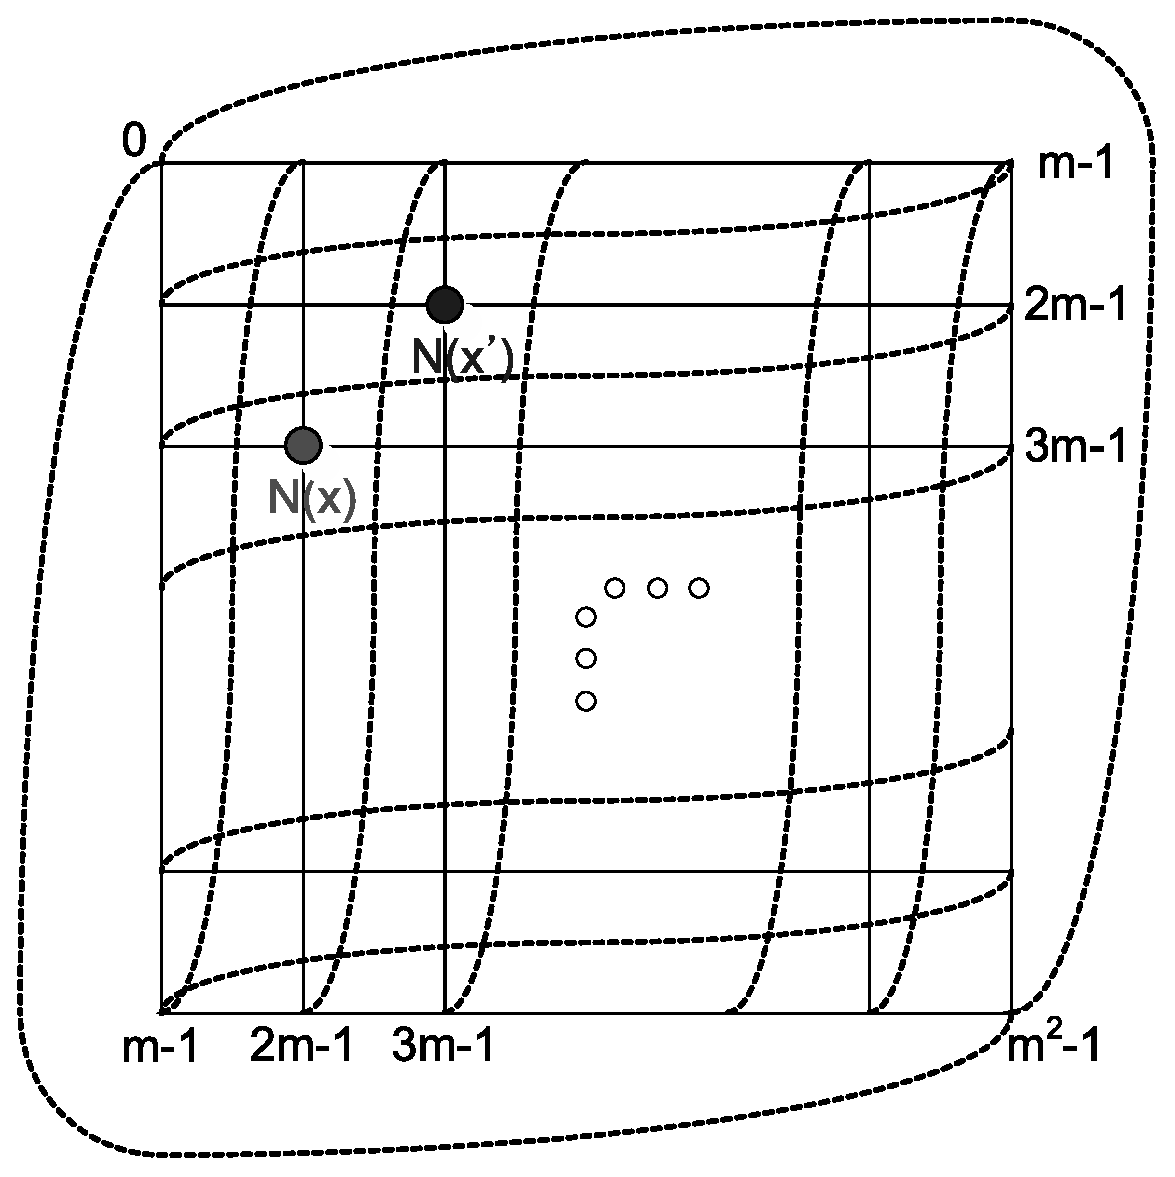
\includegraphics[width=1.2in]{figs/combined}
\caption{Overlapping of two virtual rings. This forms searching
space.} \label{fig:combined}
\end{minipage}\\
\end{tabular}
\end{figure}

\end{frame}

%\section{Algorithms}
%%%%%%%%% SLIDE %%%%%%%%%%%%%%%%
\begin{frame}
\frametitle{Caching - Data Replication}

\begin{figure}
\centering
\begin{tabular}{c|c|c}
\begin{minipage}[t]{1.3in}
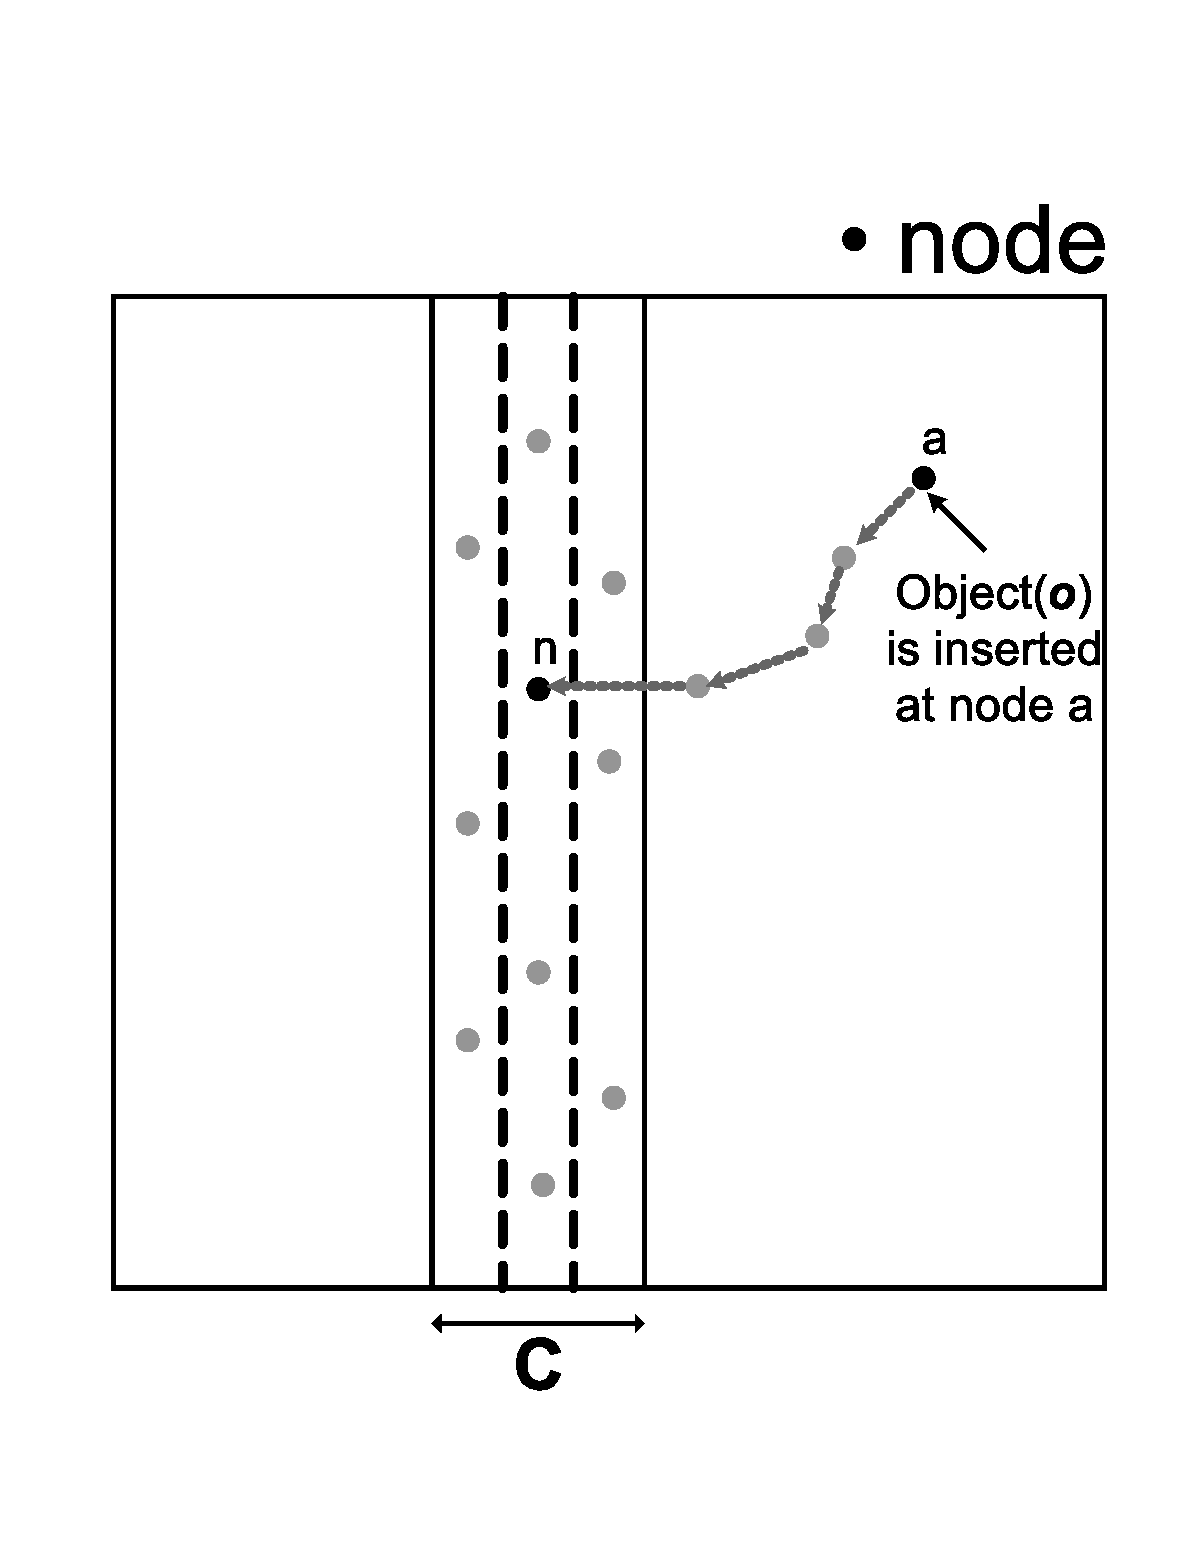
\includegraphics[width=1.2in]{figs/cache_1}
\caption{An object is inserted to a node $\textit{n}$. }
\label{fig:cache1}
\end{minipage}
& \begin{minipage}[t]{1.3in}
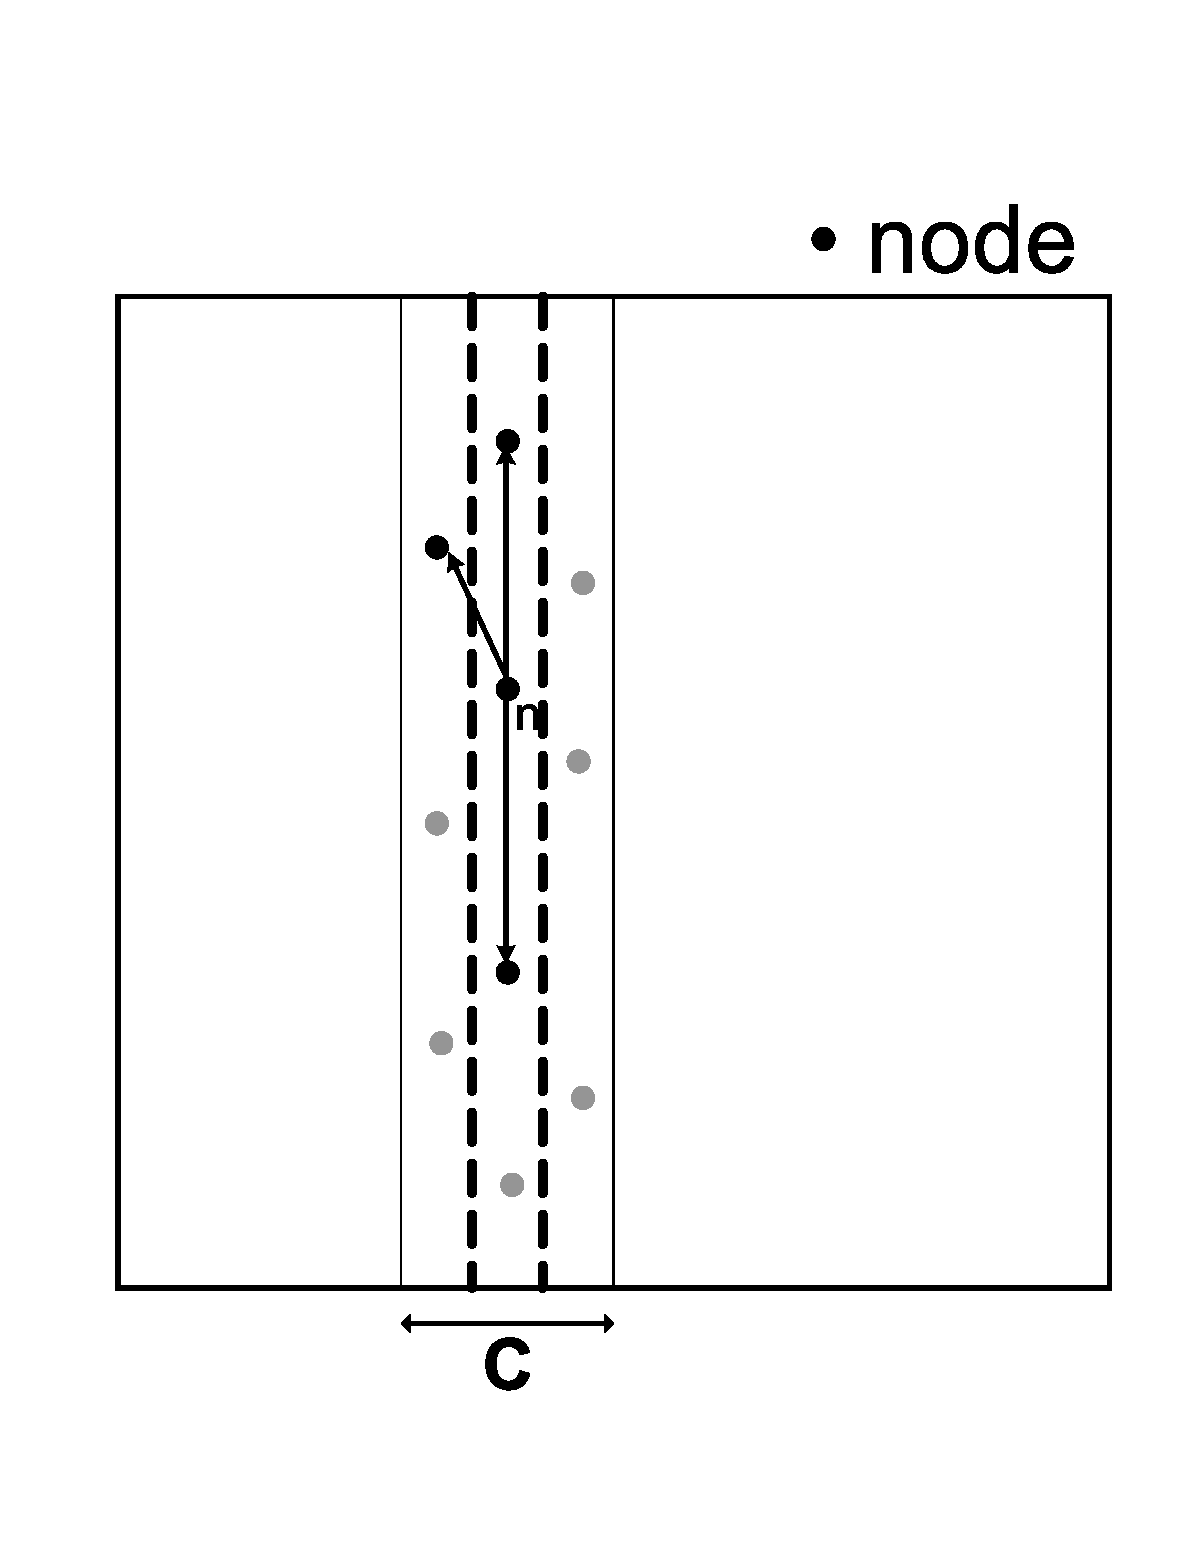
\includegraphics[width=1.2in]{figs/cache_2}
\caption{Start bounded broadcasting within $\textit{C}$.}
\label{fig:cache2}
\end{minipage}
& \begin{minipage}[t]{1.3in}
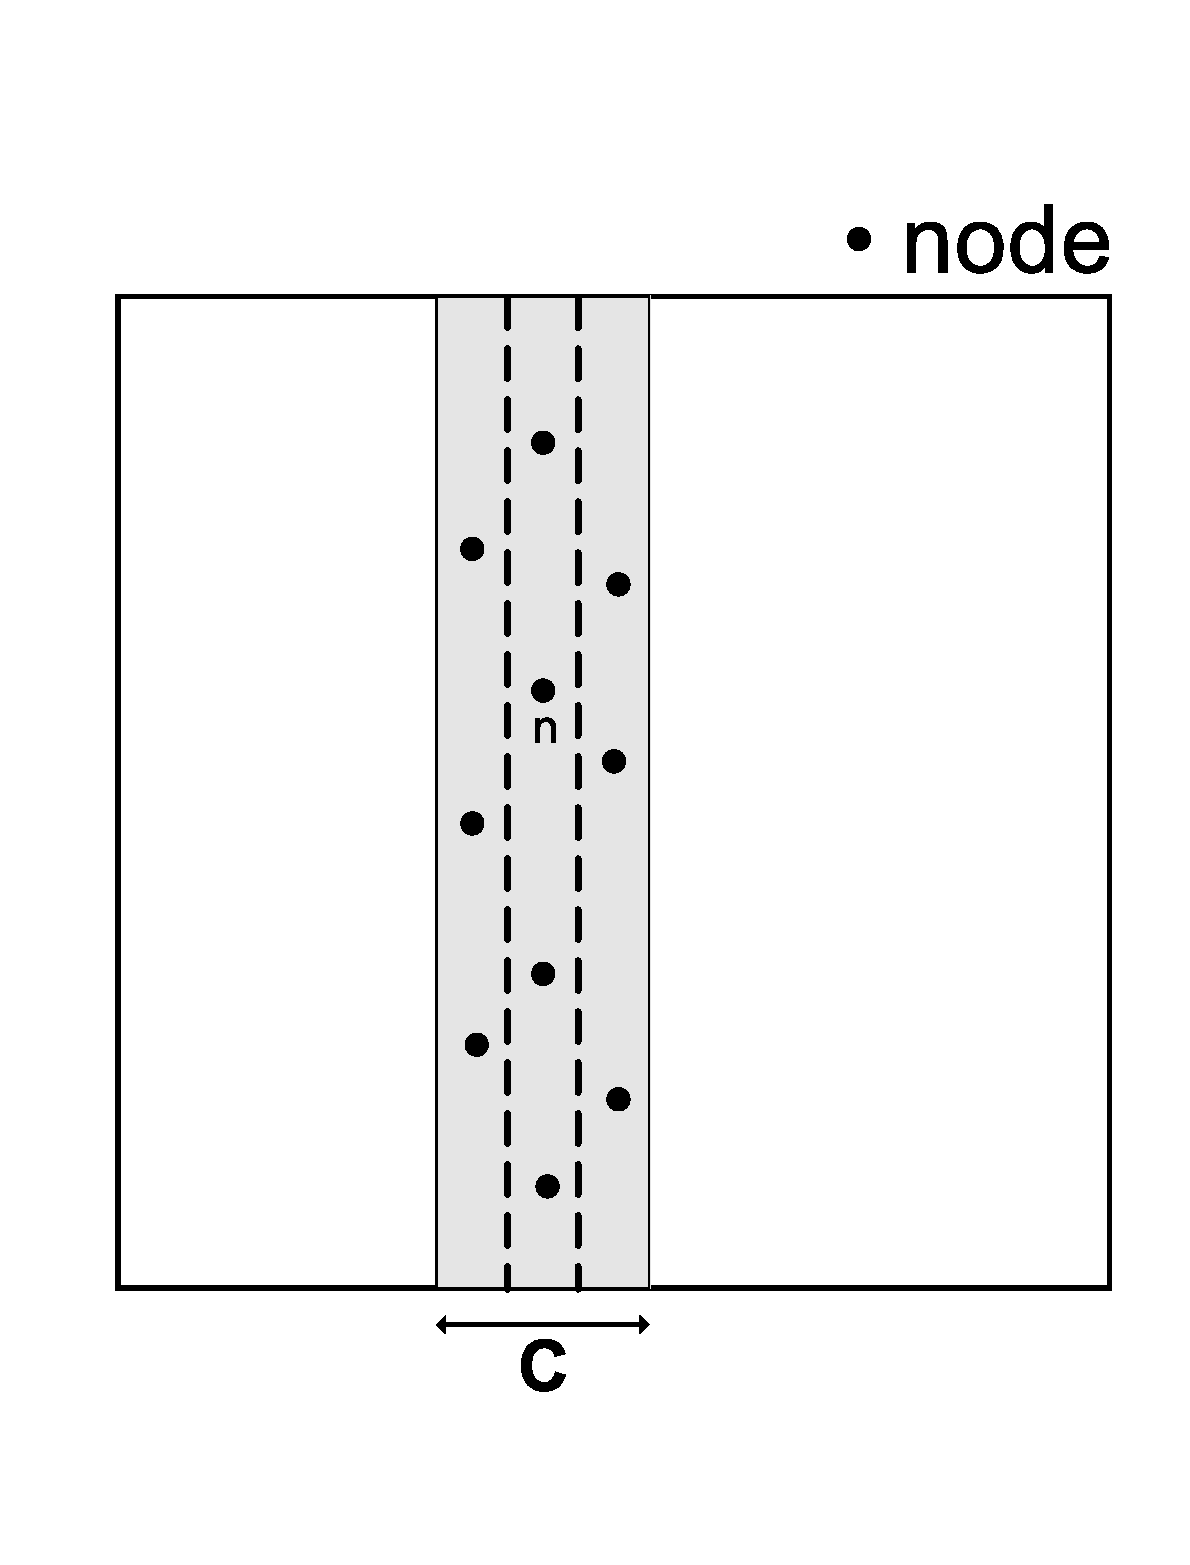
\includegraphics[width=1.2in]{figs/cache_3}
\caption{Copies of object, $\textit{o}$ is stored at every nodes in
$\textit{C}$} \label{fig:cache3}
\end{minipage}\\
\end{tabular}
\end{figure}

\end{frame}
%%%%%%%%% SLIDE %%%%%%%%%%%%%%%%
\begin{frame}
\frametitle{Query Resolution}

\begin{figure}
\centering
\begin{tabular}{c|c|c}
\begin{minipage}[t]{1.3in}
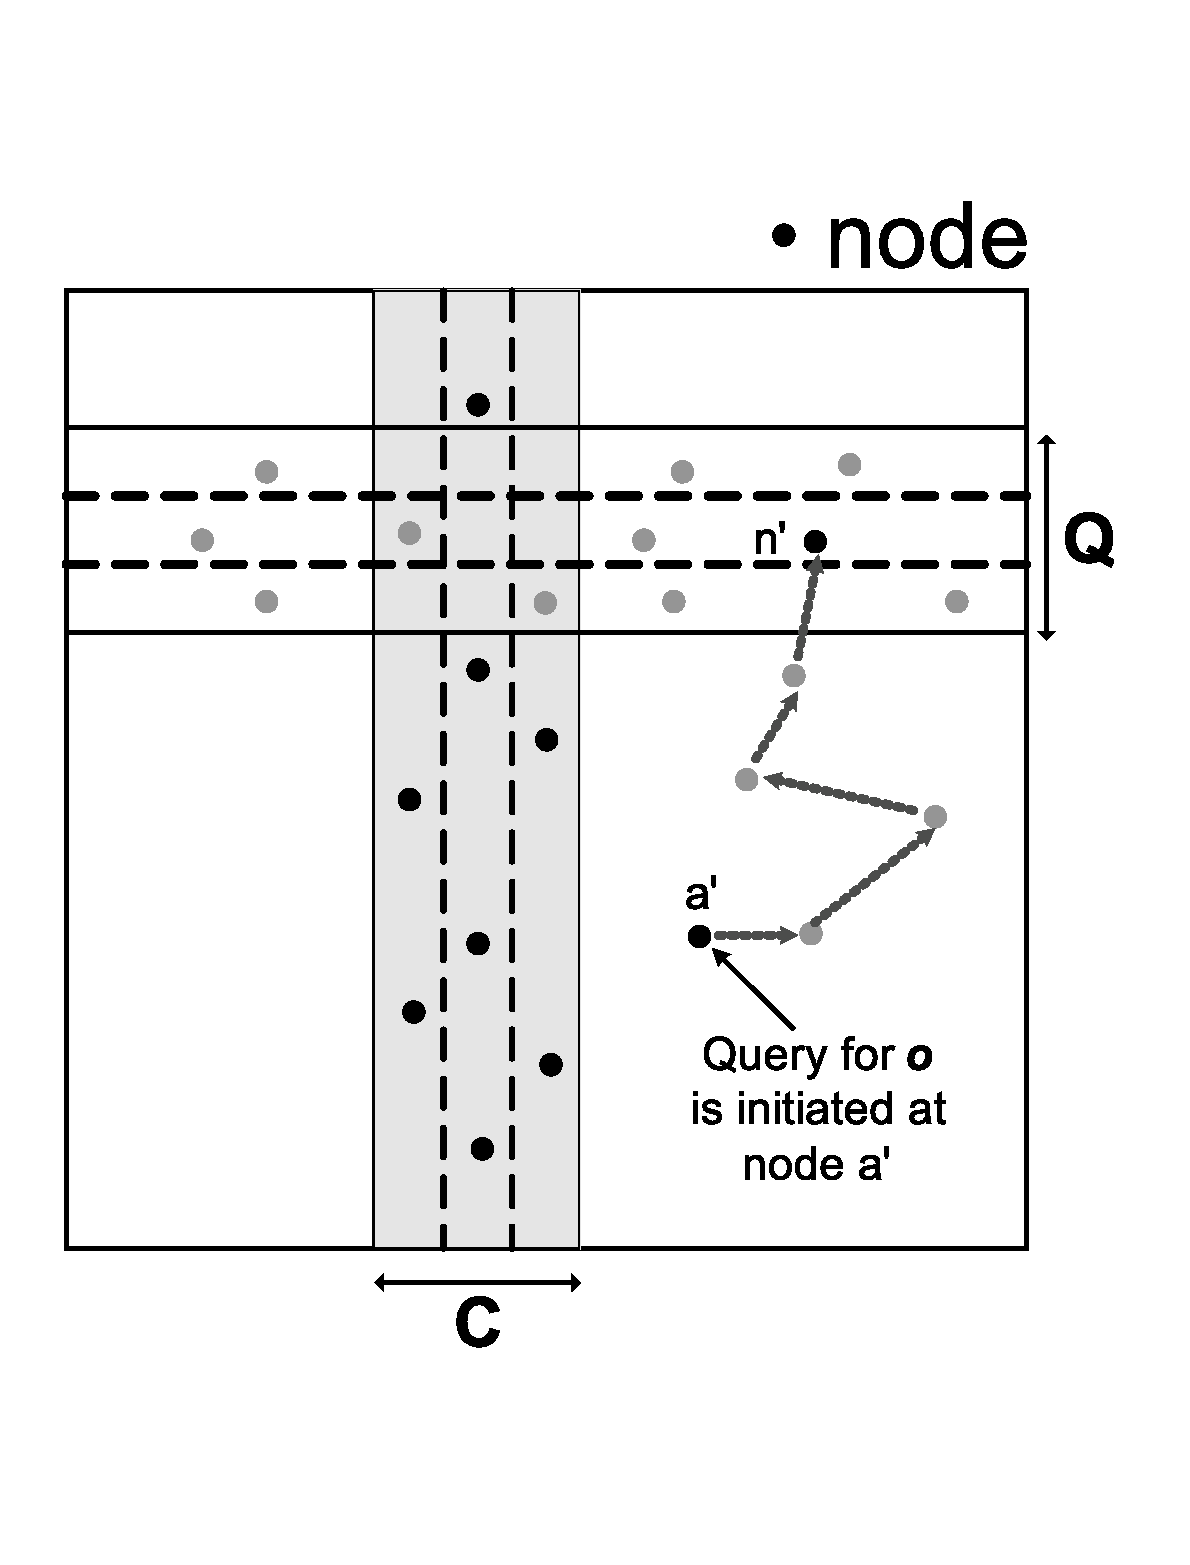
\includegraphics[width=1.2in]{figs/query_1}
\caption{A query for object $\textit{o}$ is initiated by node
n$\prime$.} \label{fig:query1}
\end{minipage}
& \begin{minipage}[t]{1.3in}
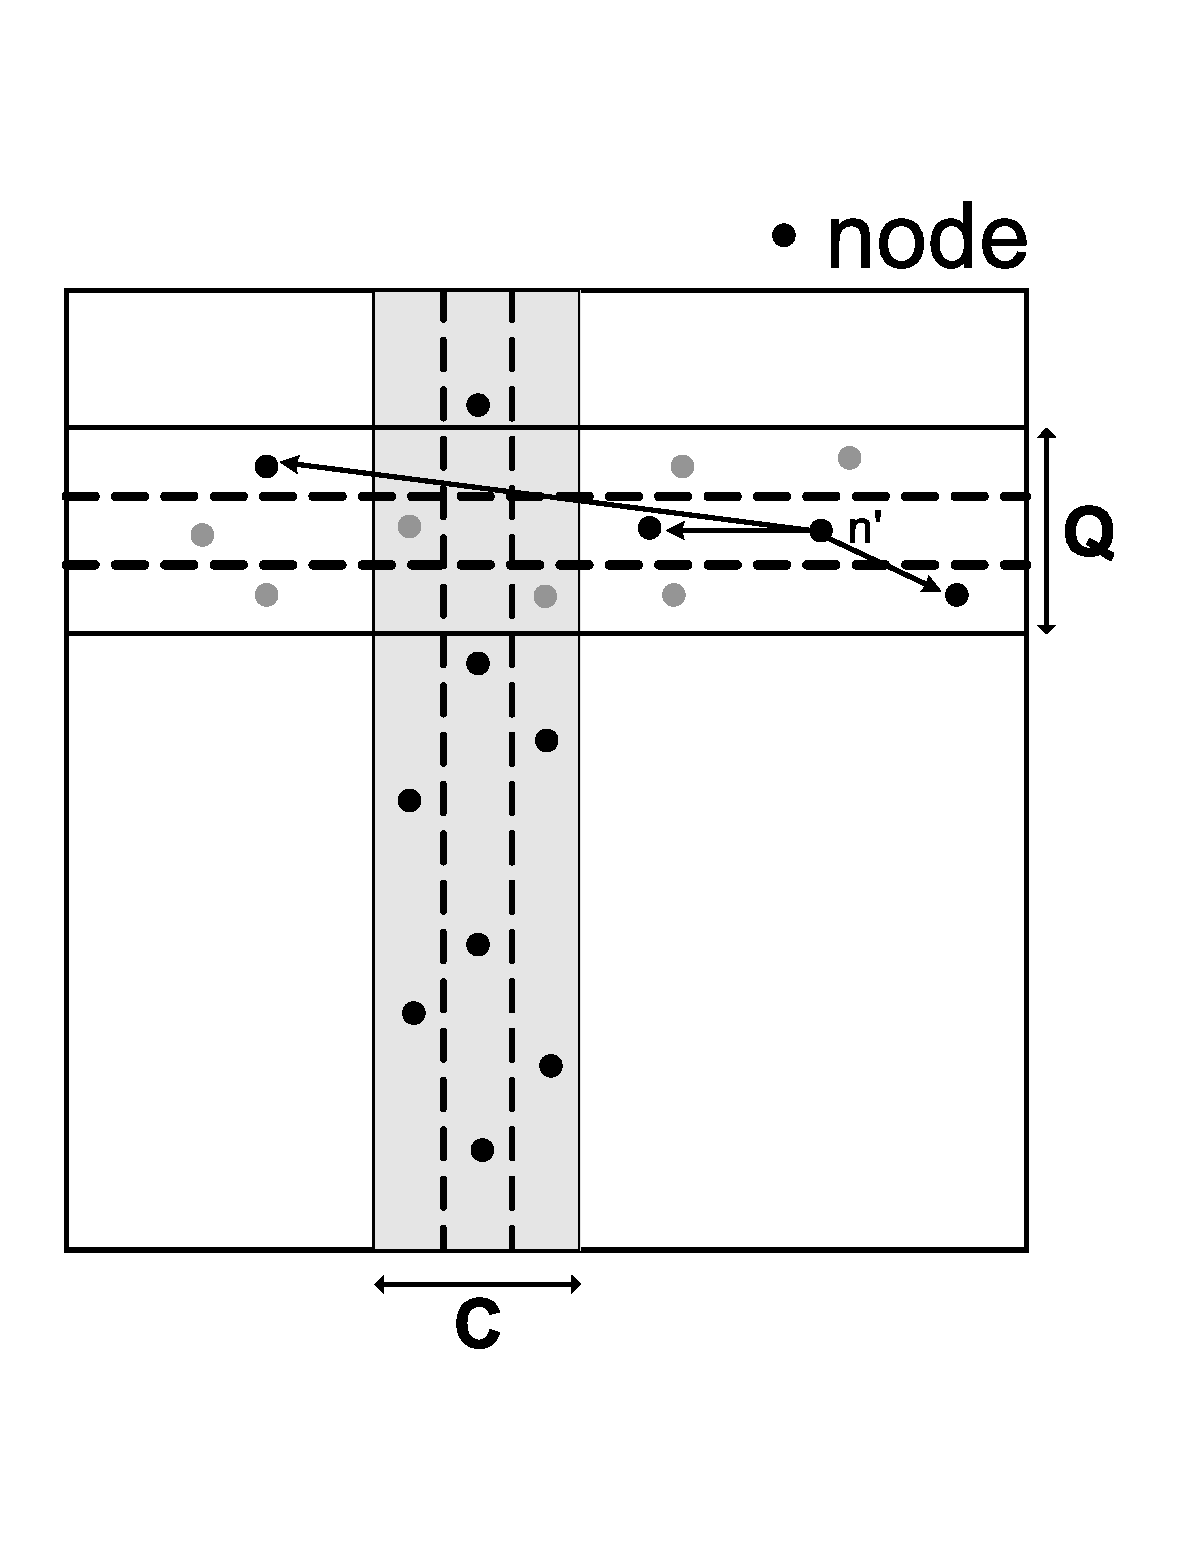
\includegraphics[width=1.2in]{figs/query_2}
\caption{n$\prime$ starts bounded broadcasting within $\textit{Q}$}
\label{fig:query2}
\end{minipage}
& \begin{minipage}[t]{1.3in}
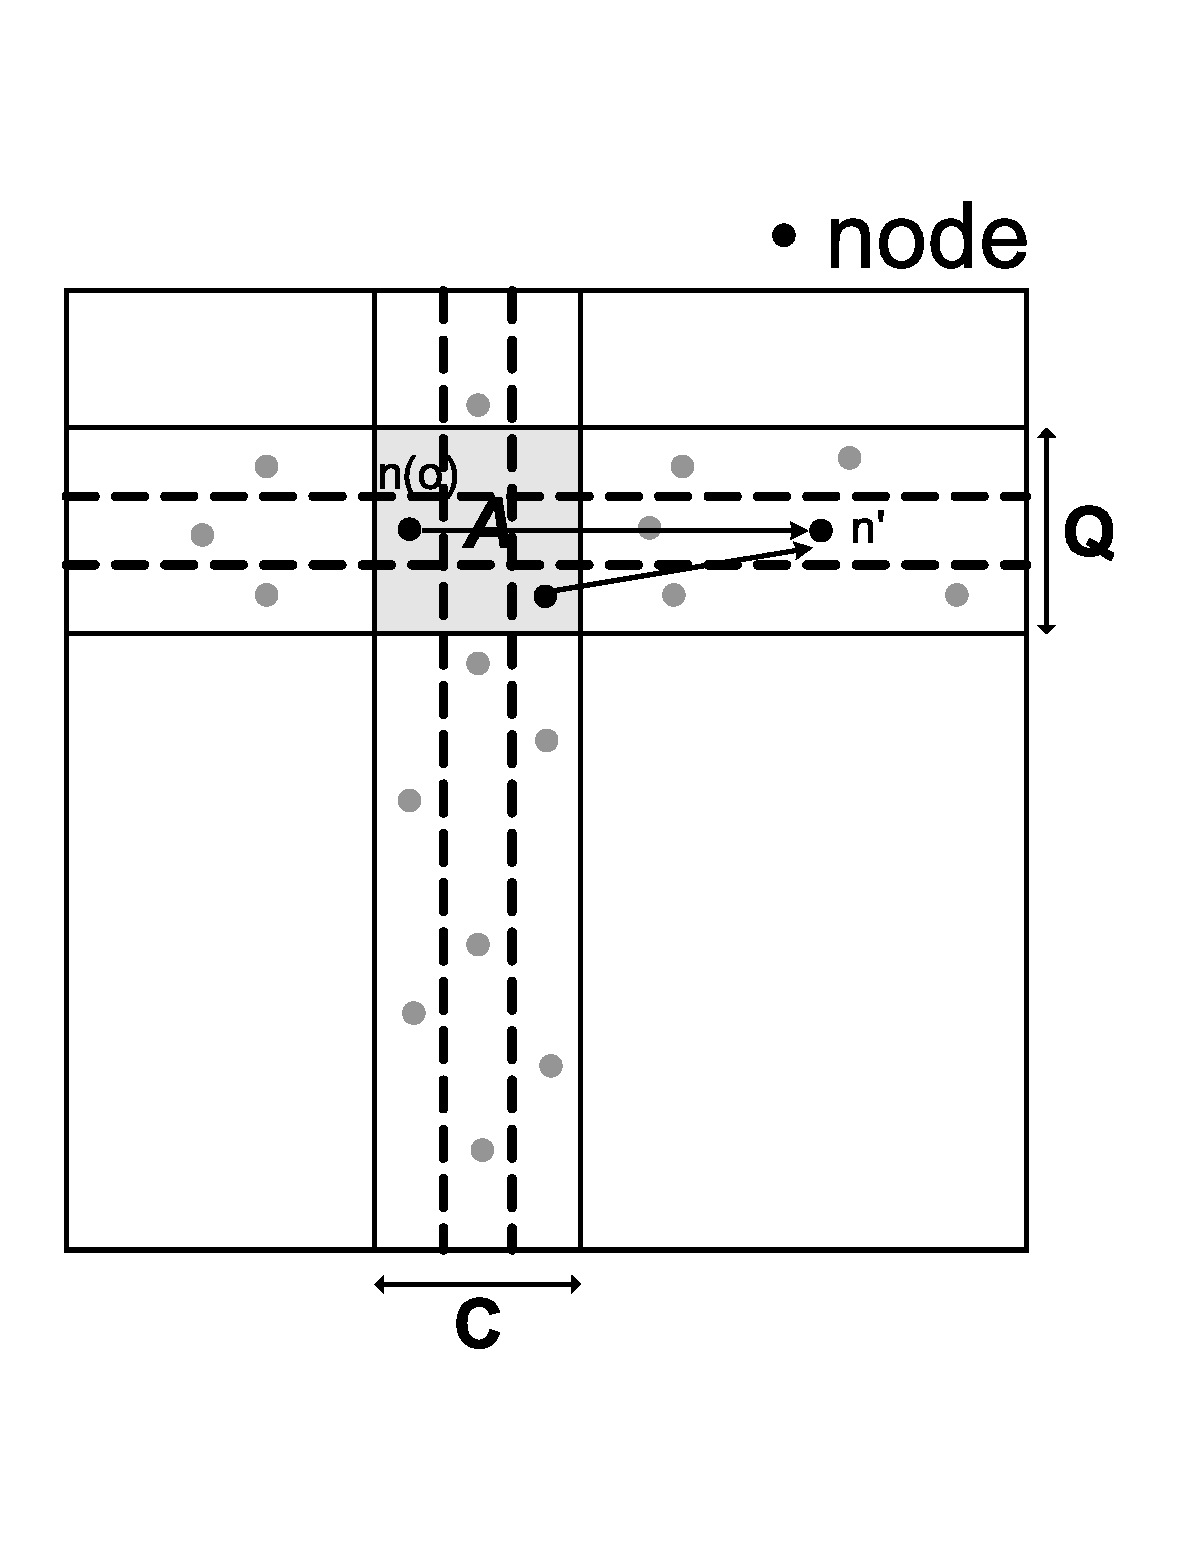
\includegraphics[width=1.2in]{figs/query_3}
\caption{Finally, n$\prime$ retrieves an object from a node n(o).}
\label{fig:query3}
\end{minipage}\\
\end{tabular}
\end{figure}
\end{frame}

%%%%%%%%% SLIDE %%%%%%%%%%%%%%%%
\begin{frame}
\frametitle{Bounded Broadcasting}
%\begin{minipage}{5cm}
\begin{itemize}
\item
Message is disseminated only to a subset of the network.
\item
Avoid massive message production
\item $O(\sqrt{N})$ cost: not as efficient as DHTs $O(\log N)$), but huge improvement over flooding-based searches ($O(N)$)
\item Build local tree
\end{itemize}
%\end{minipage}
%\begin{minipage}{5cm}
\centering
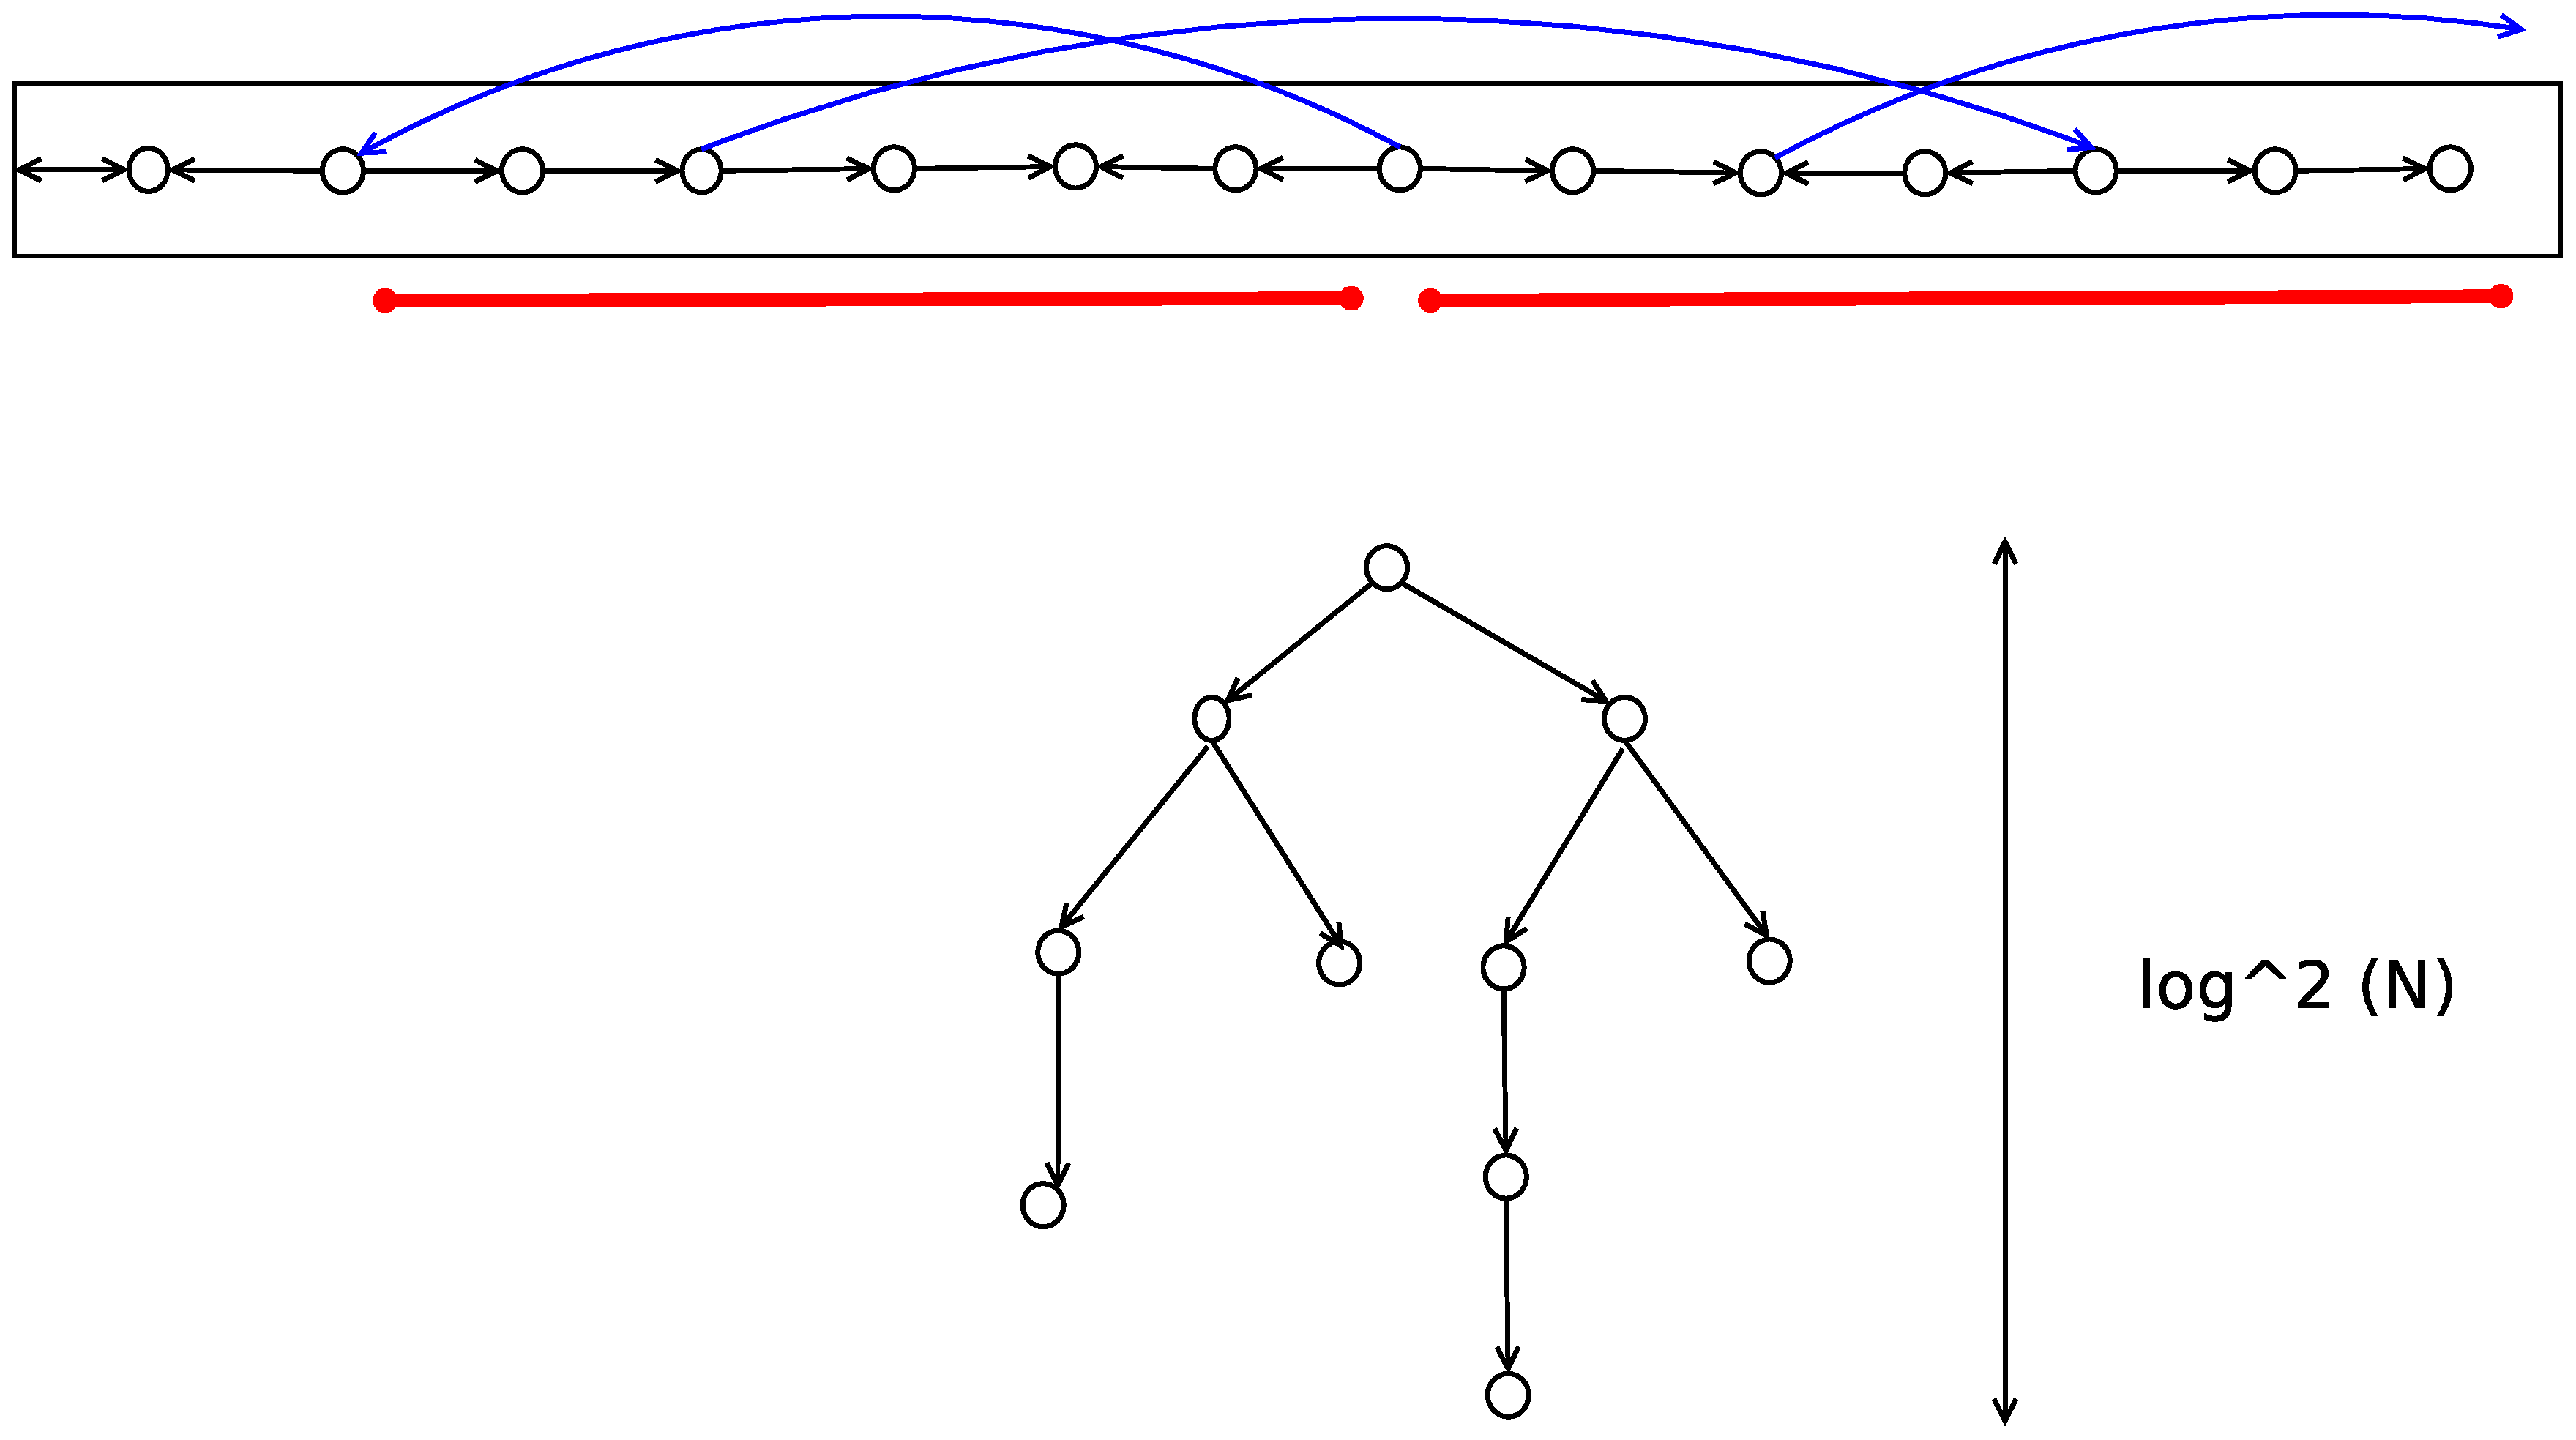
\includegraphics[scale=0.1]{figs/multi}
%\end{minipage}

\end{frame}

\iffalse
%%%%%%%%% SLIDE %%%%%%%%%%%%%%%%
\begin{frame}
\frametitle{Bounded Broadcasting - Local Tree}
\centering
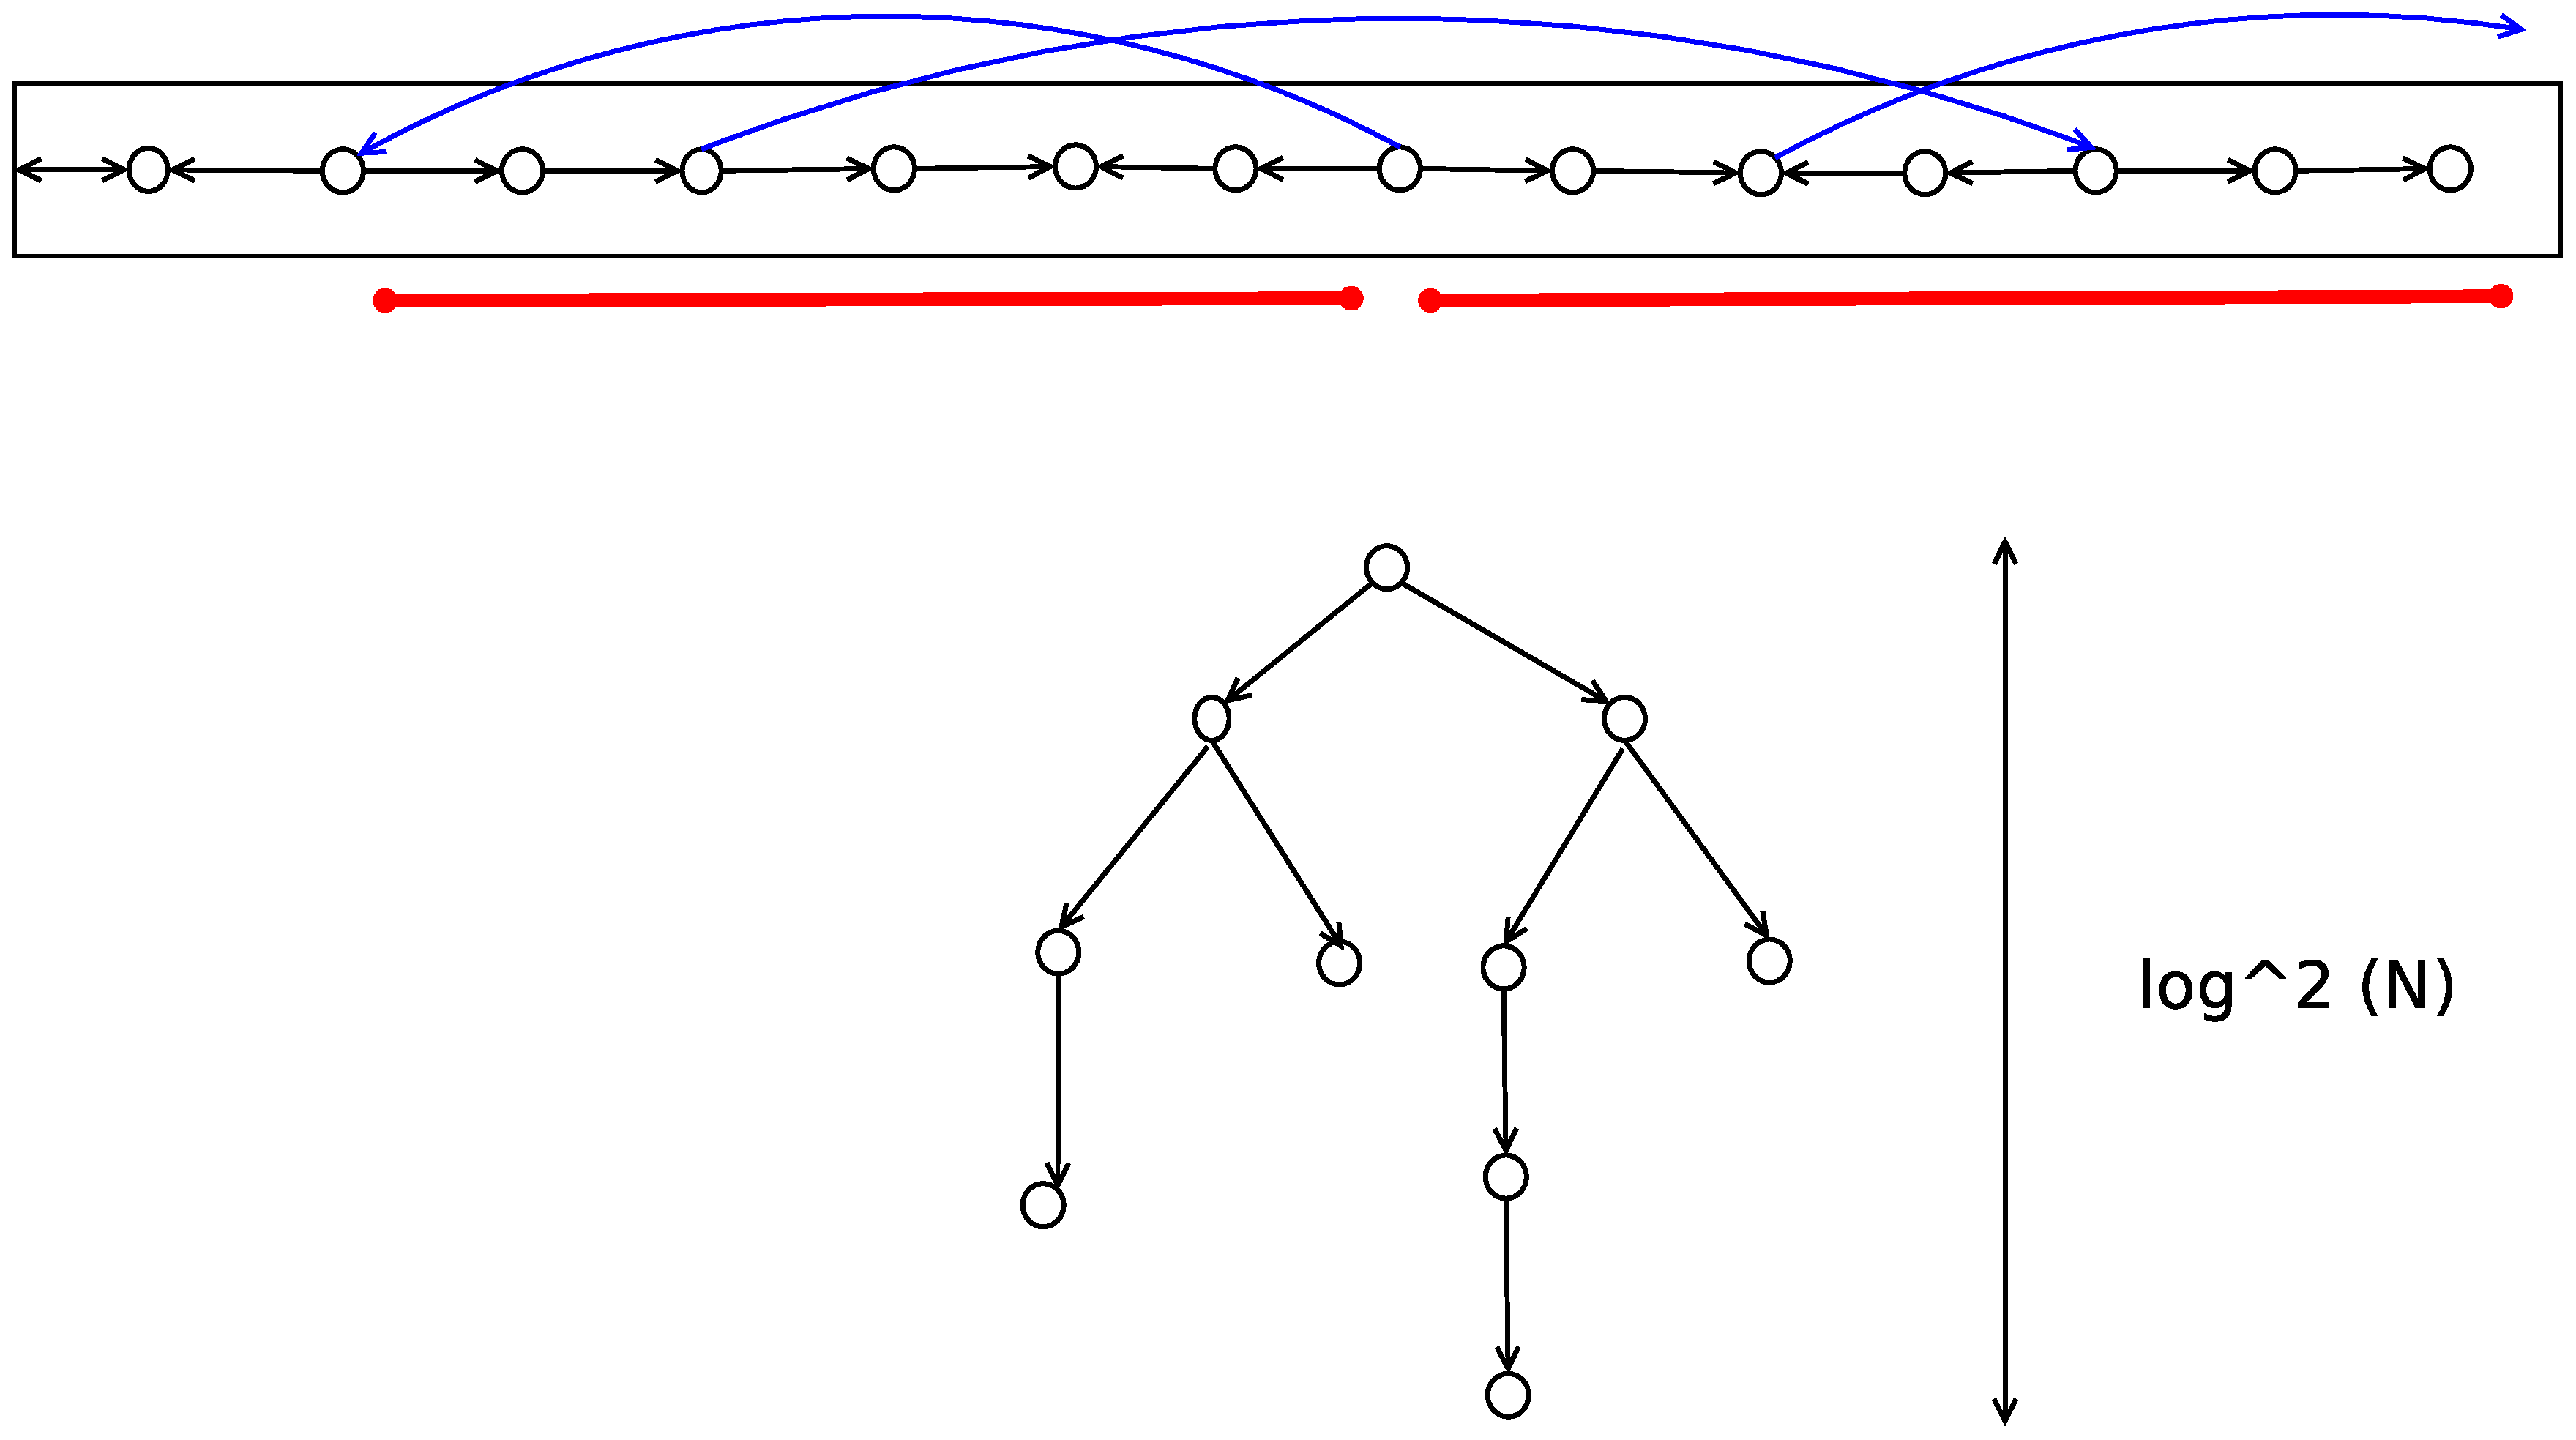
\includegraphics[scale=0.15]{figs/multi}

\end{frame}
\fi
%\section{Analysis}
%%%%%%%%% SLIDE %%%%%%%%%%%%%%%%
\begin{frame}
\frametitle{Notations}
\begin{itemize}
\item $P_s$: success rate
%\item $p$: the probability that a bin is occupied ($p = \frac{N}{B}$)
\item $p$: the probability that a bin is occupied
\item $C$: number of columns for caching
\item $Q$: number of rows for querying
\item $N$: expected number of nodes in the sapce
\item $B$: number of bins for address
\item $\alpha$: replication factor
\end{itemize}
\end{frame}
%%%%%%%%% SLIDE %%%%%%%%%%%%%%%%
\begin{frame}
\frametitle{Analysis: Success Rate}
\small{
\only<1->{
\begin{eqnarray*}
%1-P_{s} = \prod_{i=0}^{m-1}(1-p)^{c_{i}q_{i}}
1-P_{s} = \prod_{A}(1-p)
\end{eqnarray*}
}
\uncover<2->{
Then, since area \textit{A} has \textit{CQ} bins,
\begin{eqnarray*}
1-P_{s} = (1-p)^{CQ}%, where p=\frac{N}{B}
\end{eqnarray*}
}
\uncover<3->{
where $CQ$ = $\alpha$ $\frac{B}{N}$ and $p = \frac{N}{B}$
\begin{eqnarray*}%\label{th}
1-P_{s} = (1-\frac{N}{B})^{\alpha (\frac{B}{N})}
\end{eqnarray*}
}
\uncover<4->{
\begin{eqnarray*}%\label{th}
P_{s} \geq 1-e^{-\alpha} \ \ if \ \ \frac{B}{N} \rightarrow \infty 
\end{eqnarray*}
}
}
\end{frame}
%%%%%%%%% SLIDE %%%%%%%%%%%%%%%%
\begin{frame}
\frametitle{Analysis: Communication Cost}
\center
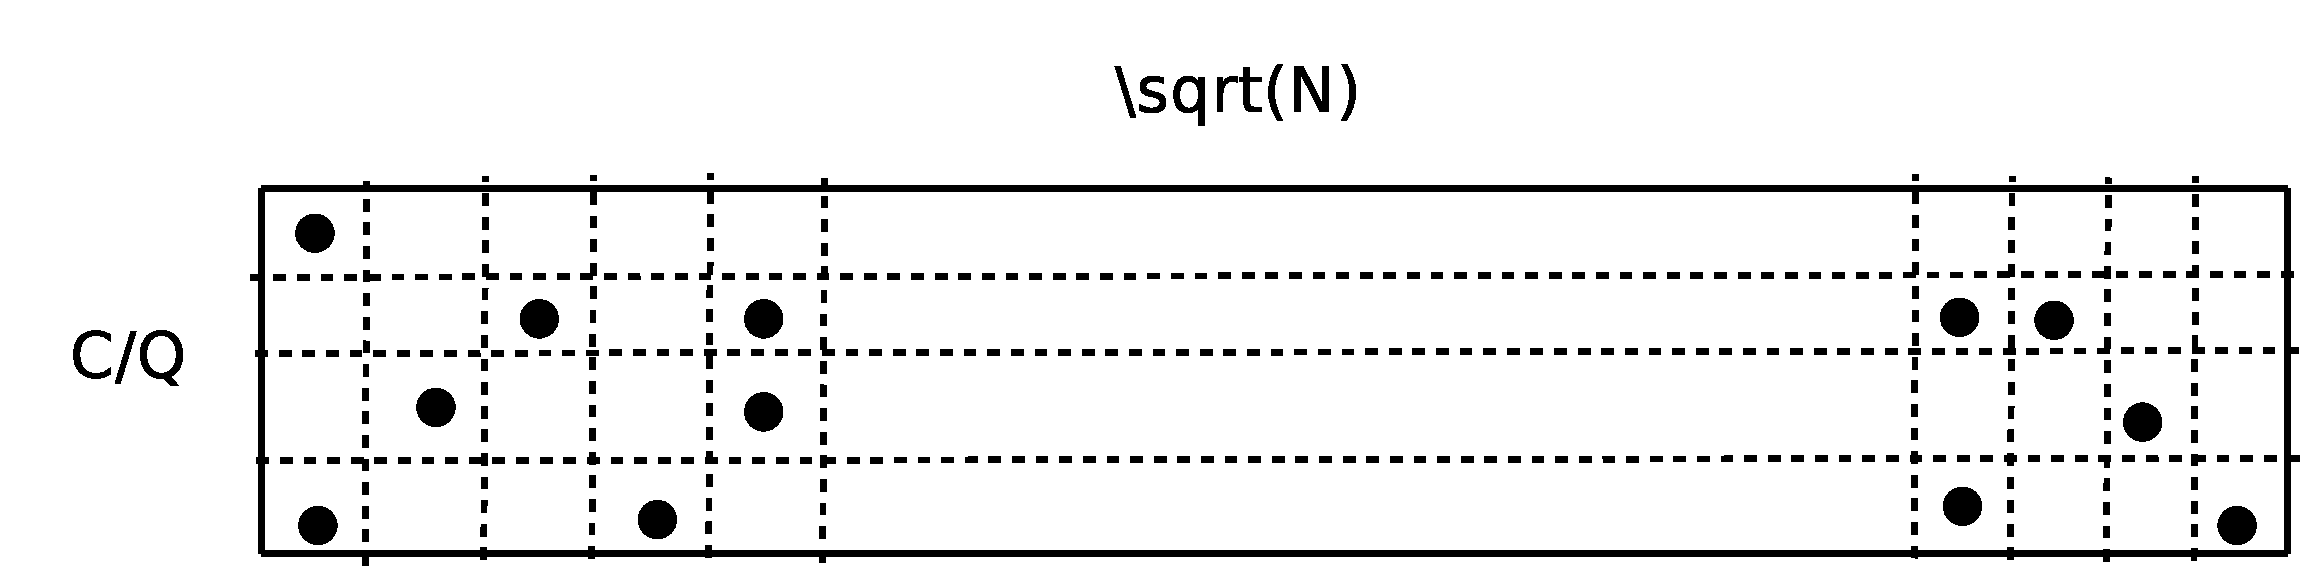
\includegraphics[scale=0.25]{figs/cost_area}

\begin{eqnarray*}\label{th}
cost &=& pC\sqrt{B}  (or\  pQ\sqrt{B})\\
  &=& \frac{N}{B}C\sqrt{B}\\
  &=& \frac{N}{B}\sqrt{\frac{\alpha B}{N}}\sqrt{B}\\
  %&=& \frac{N}{B}\sqrt{\frac{\alpha B}{N}}\sqrt{B}\\
  &=& \sqrt{\alpha N}
\end{eqnarray*}
\end{frame}
%----------------------------------------------------------------------------------
%--------------simulation results--------------------------------------------------

%\section{Simulation Results}
%%%%%%%%% SLIDE %%%%%%%%%%%%%%%%
\begin{frame}
\frametitle{Simulation Result: Success Rate}
\begin{itemize}
\item $O(1)$ hit rate with fixed $\alpha$.
\begin{eqnarray*}
P_s &=& 1-e^{-\alpha}
\end{eqnarray*}
%\item Success Rate increases exponentially w.r.t $\alpha$, independent of network size.
\end{itemize}
\center
\includegraphics[angle=270, scale=0.26]{figs/th_hitrate.eps}

\end{frame}
%%%%%%%%% SLIDE %%%%%%%%%%%%%%%%
\begin{frame}
\frametitle{Simulation Result: Communication Cost}
\begin{itemize}
\item Communication cost = $O(\sqrt{N})$
\end{itemize}
\center
\includegraphics[angle=270,scale=0.29]{figs/th_hops_loglog.eps}

\end{frame}
%%%%%%%%% SLIDE %%%%%%%%%%%%%%%%
\begin{frame}
\frametitle{Search Time}
\begin{itemize}
\item Due to small world model, forms local tree 
\item Searching in a time $O(\log^2 N)$
\end{itemize}
\begin{minipage}{5cm}
\centering
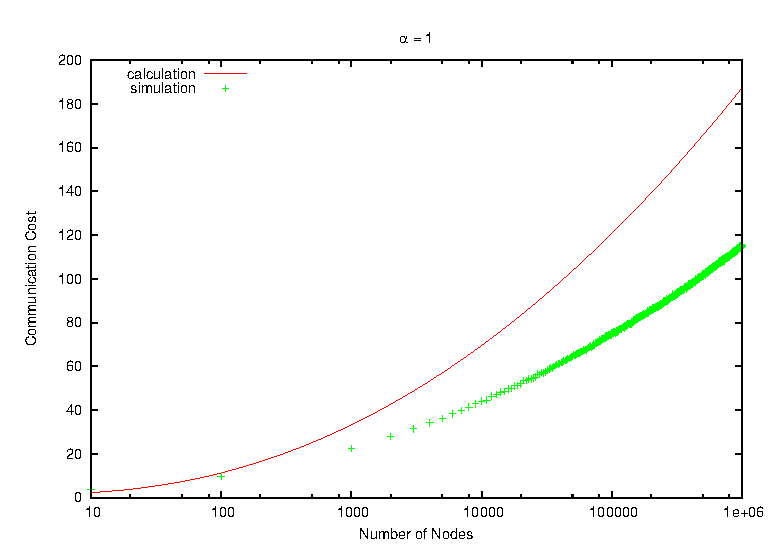
\includegraphics[scale=0.4]{figs/time1}
\end{minipage}
\begin{minipage}{5cm}
\centering
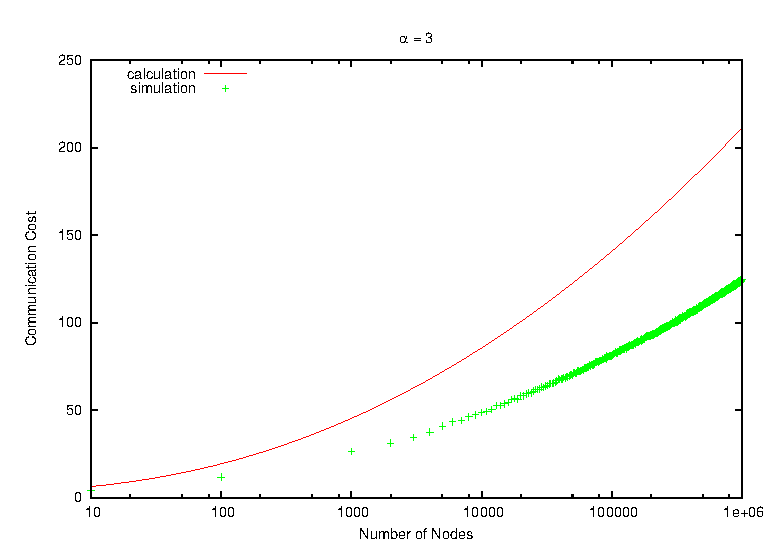
\includegraphics[scale=0.4]{figs/time3}
\end{minipage}

\end{frame}

%\section{Conclusion}
%%%%%%%%% SLIDE %%%%%%%%%%%%%%%%

\begin{frame}
\frametitle{Contribution}

\begin{itemize}
\item
Deetoo is optimal unstructured search in terms of trade-off between cache and query costs  
\item
Deetoo can resolve any kind of queries without paying high communication cost.
\item Deetoo can update, delete data objects unlikely to other unstructured systems
\item
We built hit-rate controllable caching and querying.
\item
Deetoo can be a good search tool for P2P networks.
\end{itemize}
\end{frame}

%~~~~~~~~~~~~~~~~~~~~~~~~~~~~~~~~~~~~~~~~~~~~~~~~~~~~~~%
\section{Deetoo Implementation and Deployment}
\frame<beamer>{\tableofcontents[current]}
%%%%%%%%% SLIDE %%%%%%%%%%%%%%%%
\begin{frame}
\frametitle{Deetoo Implementation on Real Network}
\begin{itemize}
\item Real implementation of Deetoo on Planet-Lab network
\item Writing an API to make it easy for people to make new query and cache objects.
\end{itemize}
\end{frame}

%%%%%%%%% SLIDE %%%%%%%%%%%%%%%%
\begin{frame}
\frametitle{System Model}
\begin{itemize}
\item Overlay Network - Brunet
\item Network Size Estimator
\item MapReduce based Cache/Query system
\end{itemize}
\end{frame}

%%%%%%%%% SLIDE %%%%%%%%%%%%%%%%
\begin{frame}
\frametitle{Brunet}
\begin{itemize}
\item 
\item 
\end{itemize}
\end{frame}

%%%%%%%%% SLIDE %%%%%%%%%%%%%%%%
\begin{frame}
\frametitle{P2P Network Overview}
\begin{center}
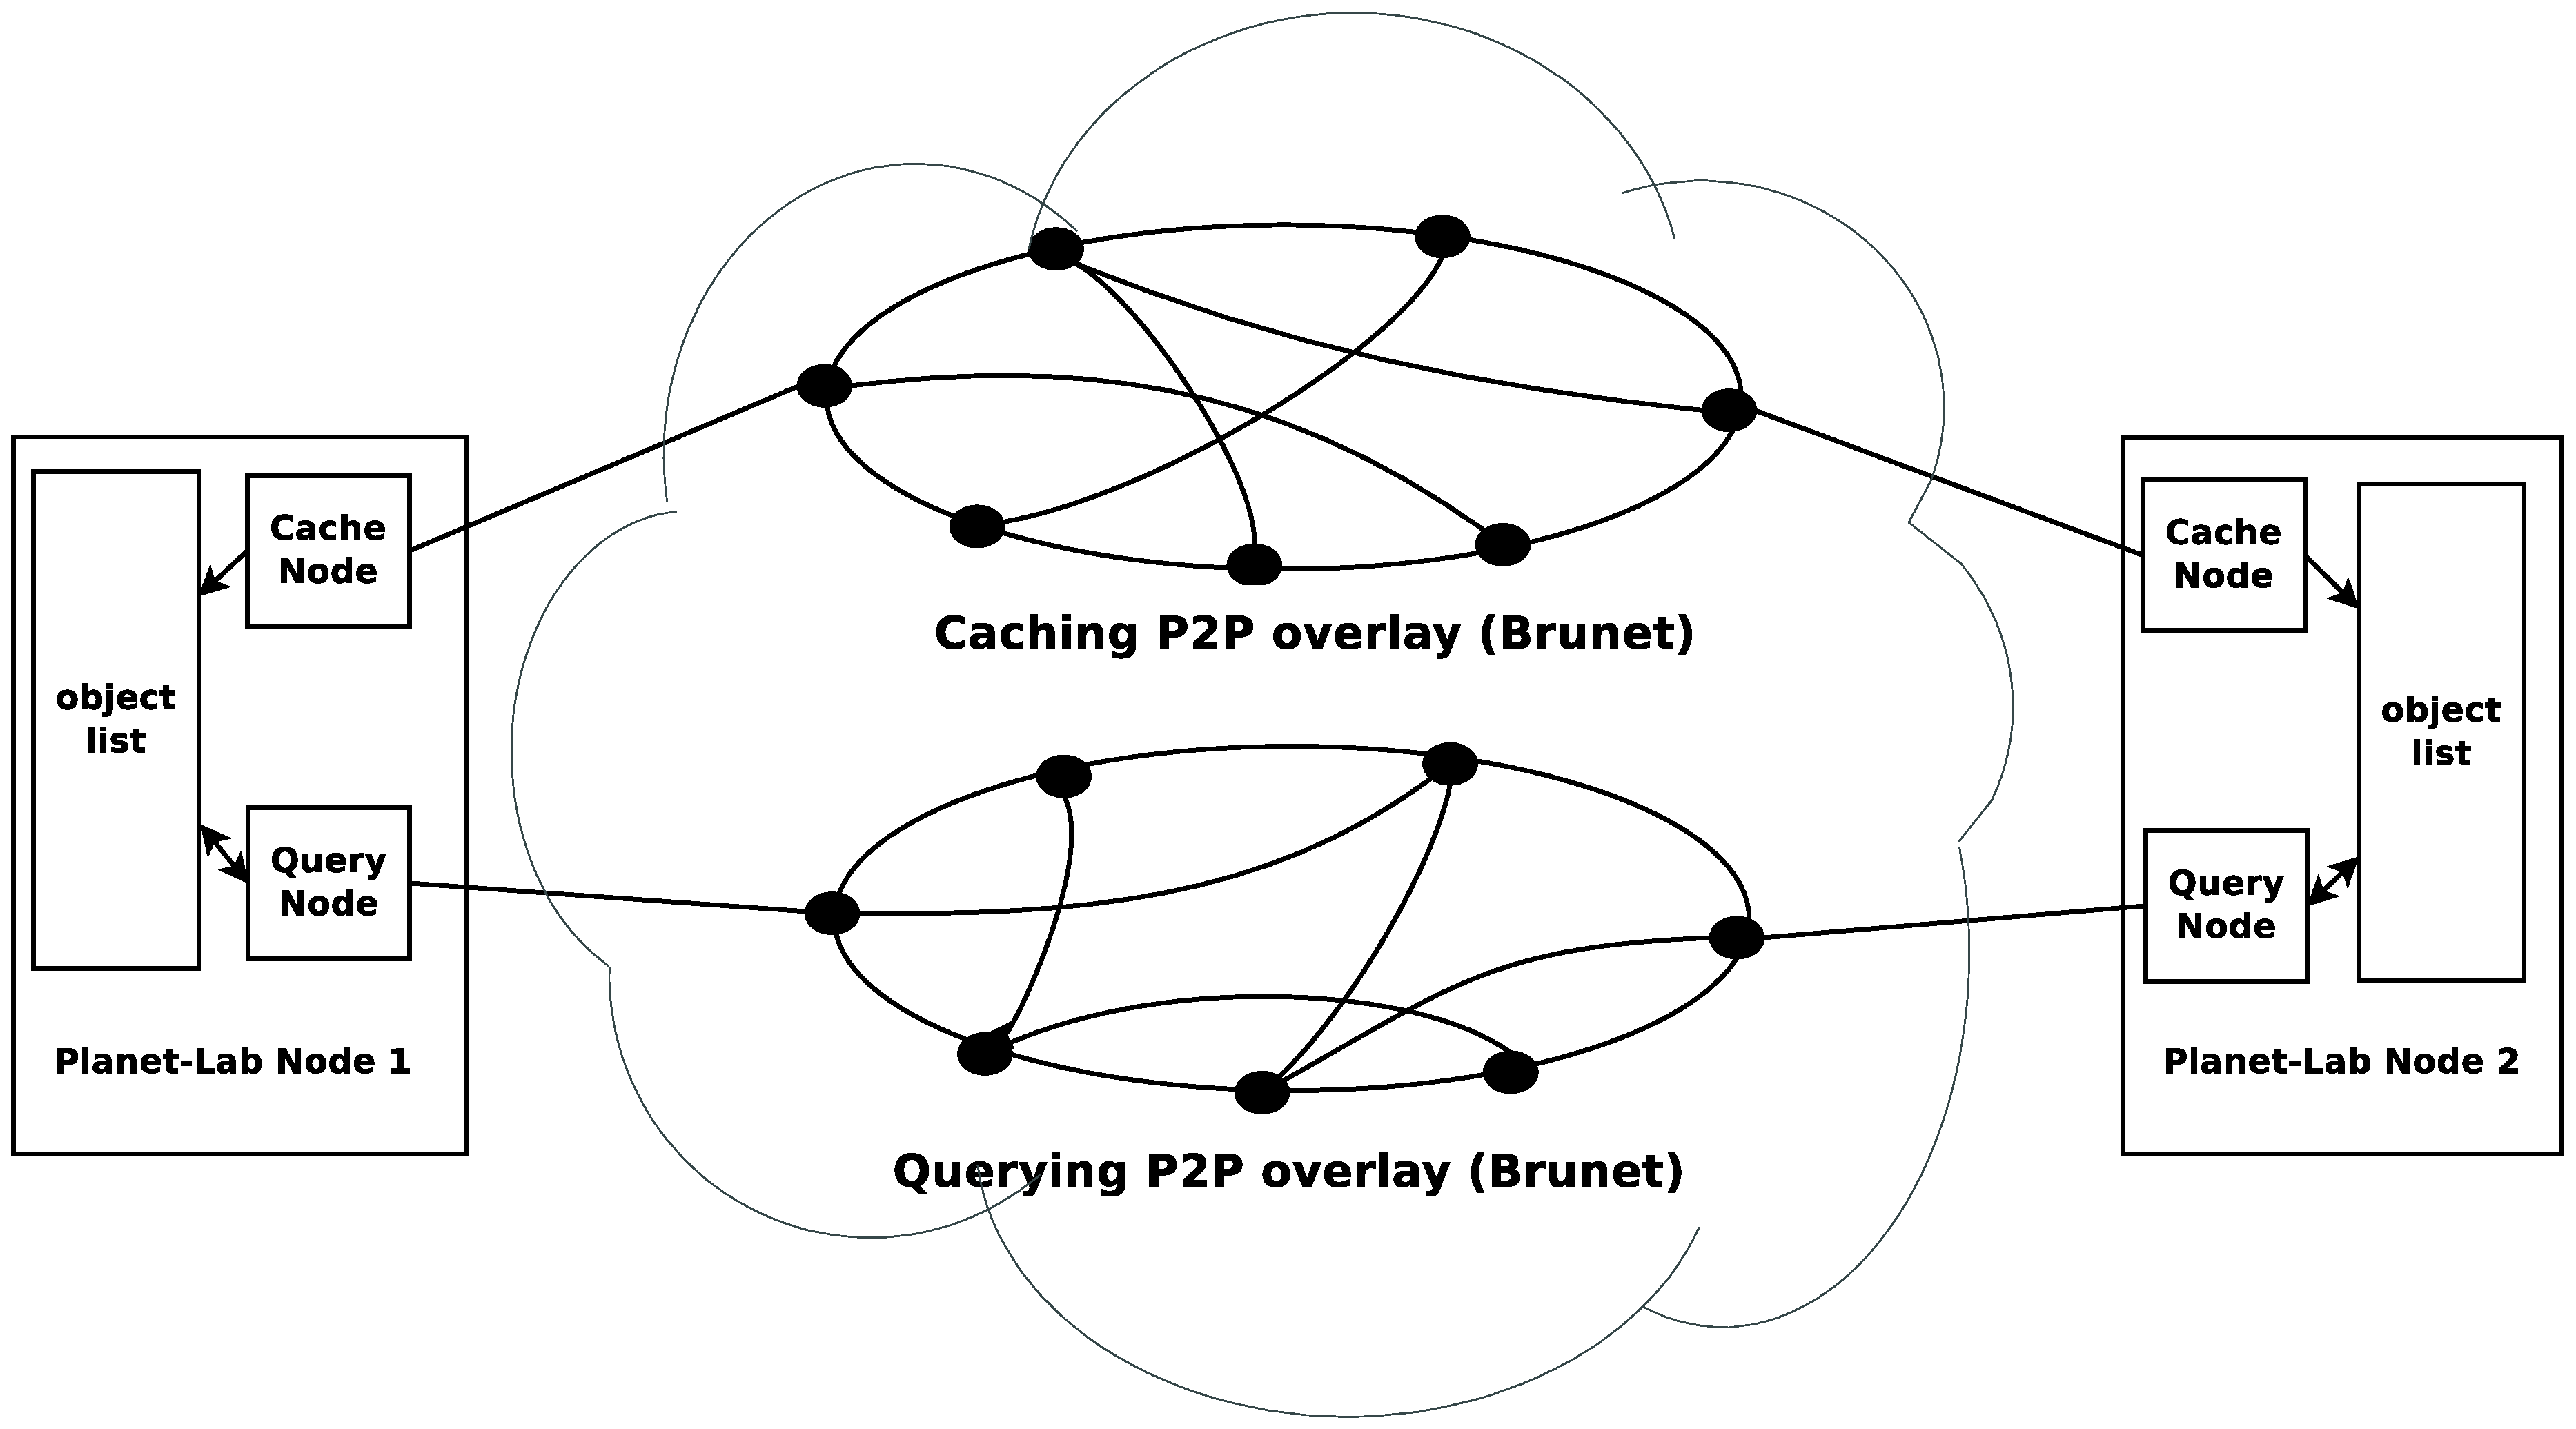
\includegraphics[scale=0.17]{figs/brunet}
\end{center}
\end{frame}

%%%%%%%%% SLIDE %%%%%%%%%%%%%%%%
\begin{frame}
\frametitle{MapReduce Modules}
\begin{itemize}
\item 
\item 
\end{itemize}
\end{frame}

%%%%%%%%% SLIDE %%%%%%%%%%%%%%%%
\begin{frame}
\frametitle{MapReduce Functional Modules}
\begin{center}
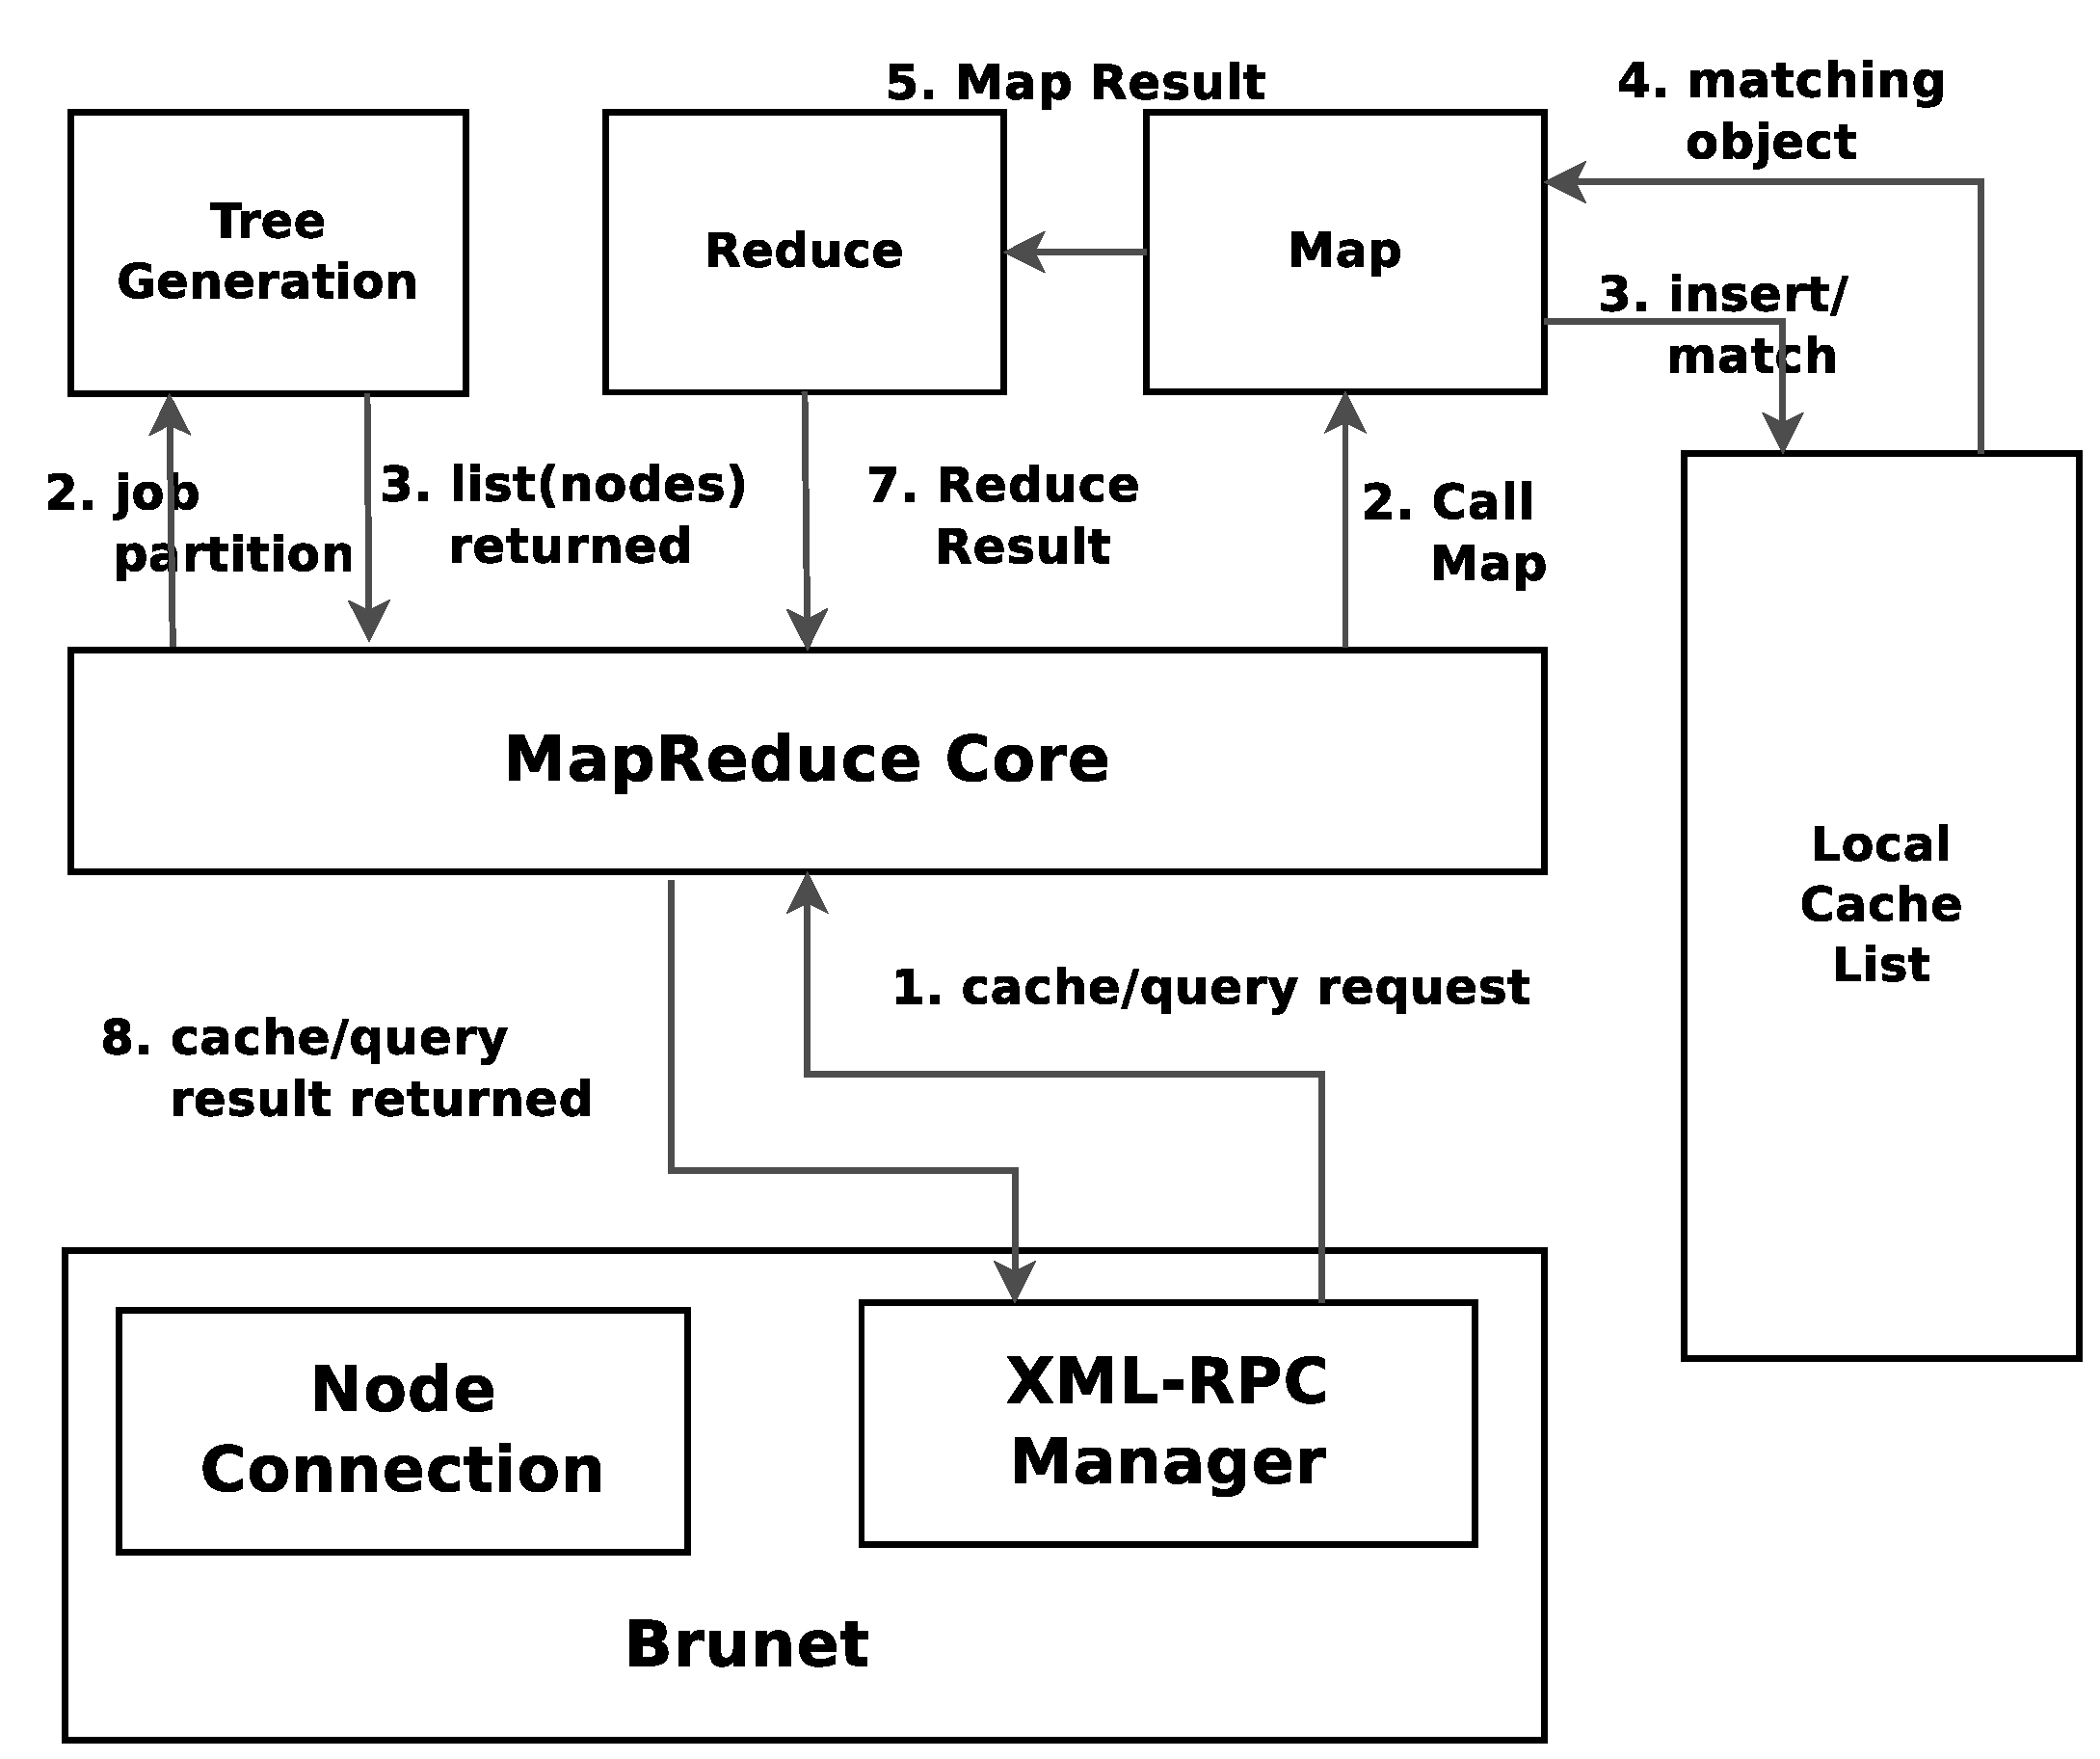
\includegraphics[scale=0.2]{figs/mapreduce_query_system}
\end{center}
\end{frame}

%%%%%%%%% SLIDE %%%%%%%%%%%%%%%%
\begin{frame}
\frametitle{Experimental Environment}
\begin{itemize}
\item 
\item 
\end{itemize}
\end{frame}

%%%%%%%%% SLIDE %%%%%%%%%%%%%%%%
\begin{frame}
\frametitle{}
\begin{itemize}
\item 
\item 
\end{itemize}
\end{frame}


%%%%%%%%% SLIDE %%%%%%%%%%%%%%%%
\begin{frame}
\frametitle{Results: hit rate}
\begin{itemize}
\item 
\end{itemize}
\begin{center}
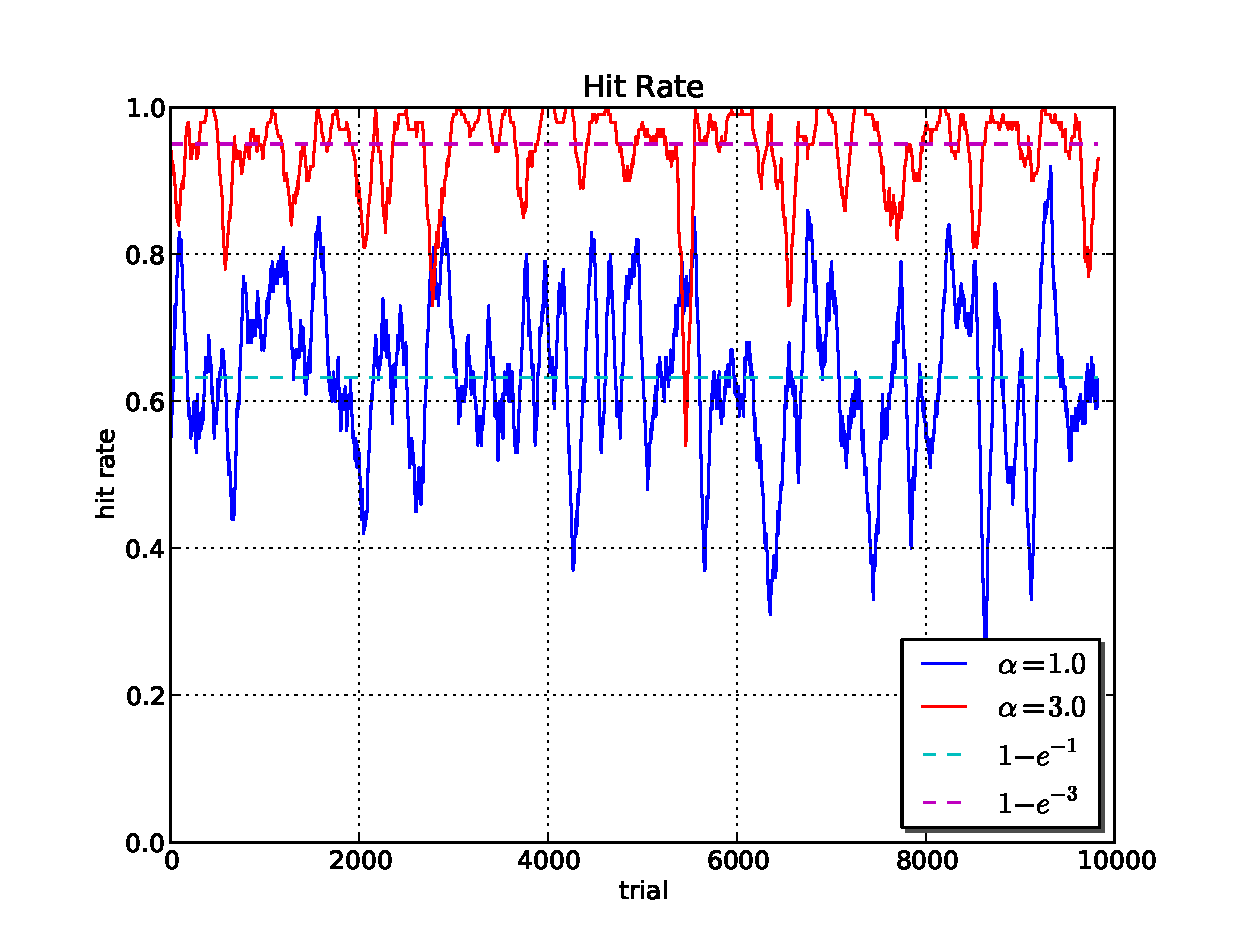
\includegraphics[scale=0.4]{figs/plab_hit.eps}
\end{center}
\end{frame}

%%%%%%%%% SLIDE %%%%%%%%%%%%%%%%
\begin{frame}
\frametitle{Results: Cost}
\begin{itemize}
\item 
\end{itemize}
\begin{center}
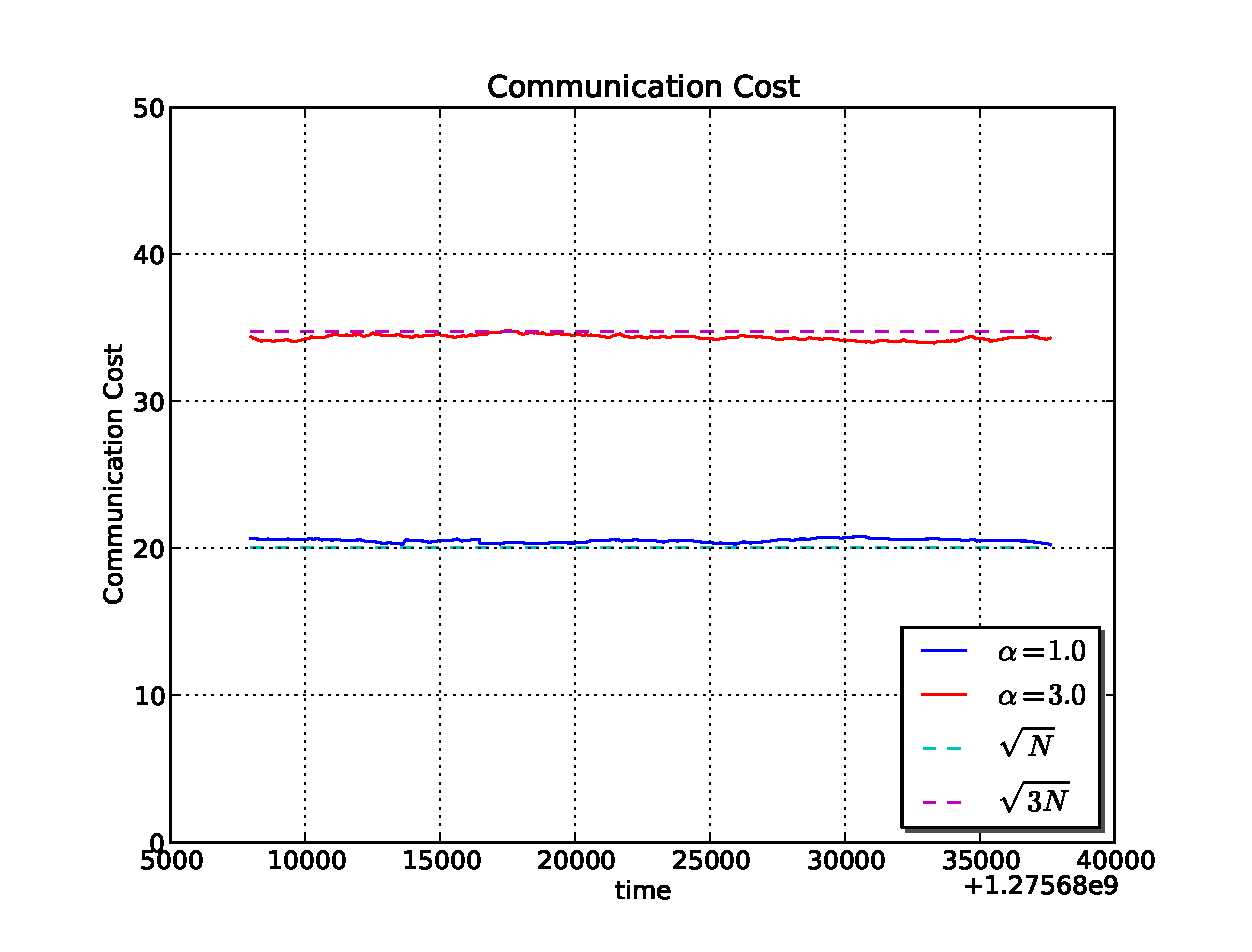
\includegraphics[scale=0.4]{figs/plab_cost.eps}
\end{center}
\end{frame}

%%%%%%%%% SLIDE %%%%%%%%%%%%%%%%
\begin{frame}
\frametitle{Results: Search Time}
\begin{itemize}
\item 
\end{itemize}
\begin{center}
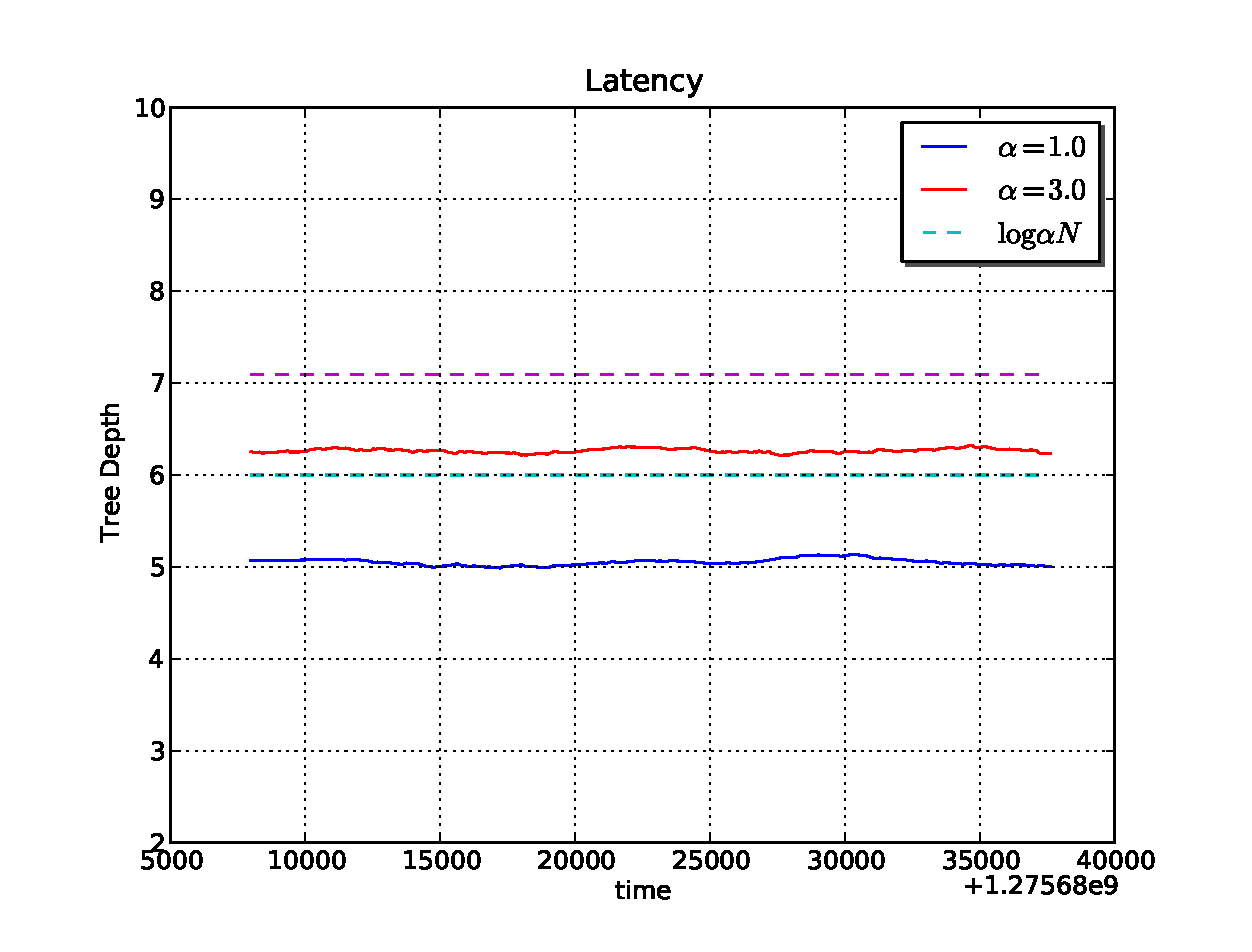
\includegraphics[scale=0.4]{figs/plab_depth.eps}
\end{center}
\end{frame}

%%%%%%%%% SLIDE %%%%%%%%%%%%%%%%
\begin{frame}
\frametitle{Results: Network Size Estimation}
\begin{itemize}
\item 
\end{itemize}
\begin{center}
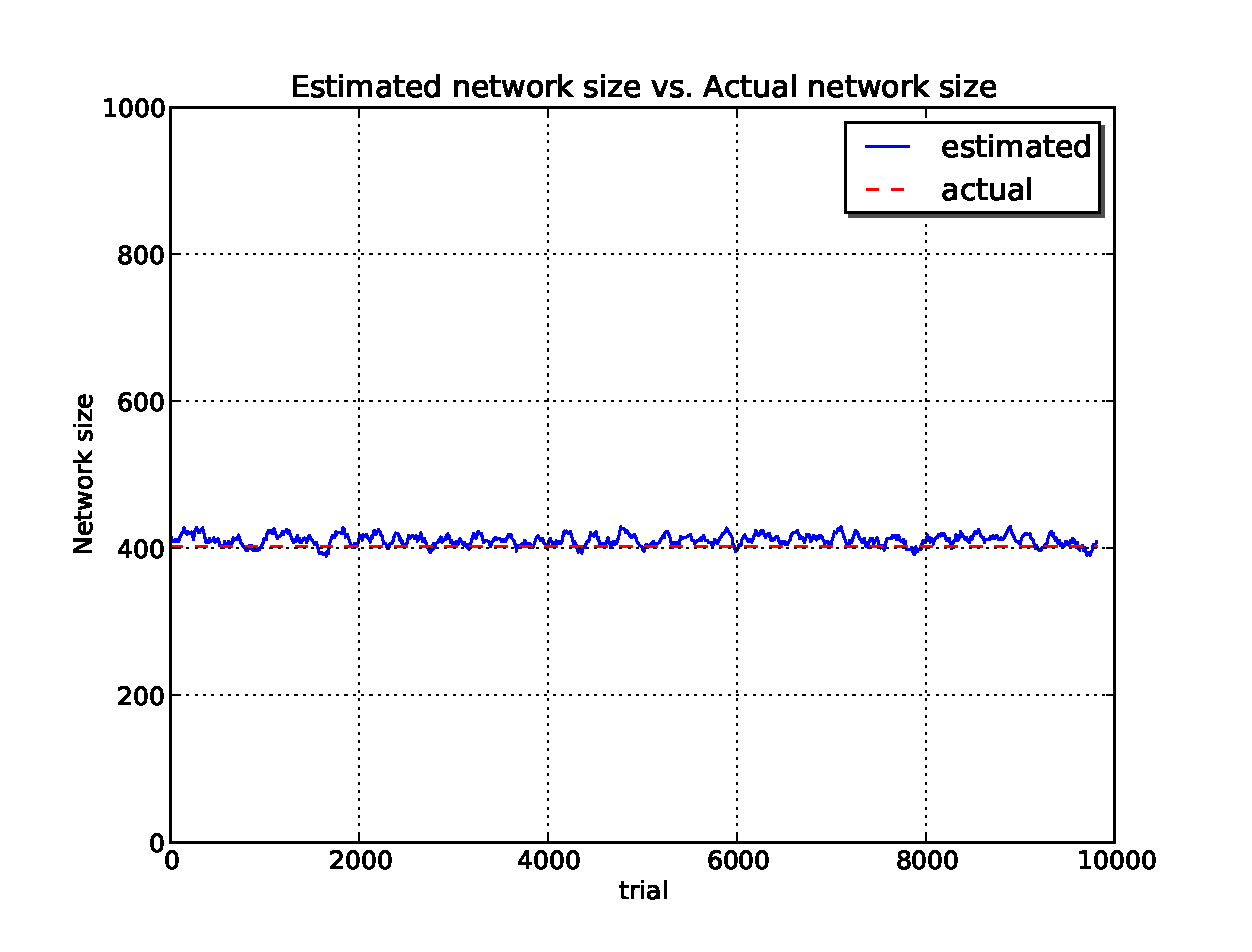
\includegraphics[scale=0.4]{figs/plab_size.eps}
\end{center}
\end{frame}

%%%%%%%%% SLIDE %%%%%%%%%%%%%%%%
\begin{frame}
\frametitle{Conclusion}
\begin{itemize}
\item 
\item 
\end{itemize}
\end{frame}

%~~~~~~~~~~~~~~~~~~~~~~~~~~~~~~~~~~~~~~~~~~~~~~~~~~~~~~%
\section{Exact Deetoo}
\frame<beamer>{\tableofcontents[current]}

%%%%%%%%% SLIDE %%%%%%%%%%%%%%%%
\begin{frame}
\frametitle{Exact Deetoo: The Motivation}
\begin{itemize}
\item Deetoo achieves constant hit rate.
\item How can Deetoo achieve 100\% hit rate without paying more cost?
\end{itemize}
\end{frame}
%%%%%%%%% SLIDE %%%%%%%%%%%%%%%%
%\begin{frame}
%\frametitle{Adaptive Deetoo}
%\begin{itemize}
%\item Refine Deetoo using feedback
%\item Cache/Query action results include the number of nodes in a given range.
%\item Using this information, we can improve the network size estimation
%\item In case of cache, maintaining square root replication is very important.
%\item No additional communication cost is required.
%\end{itemize}
%\end{frame}

%%%%%%%%% SLIDE %%%%%%%%%%%%%%%%
\begin{frame}
\frametitle{The Algorithm}
\begin{itemize}
\item Join
\item Split
\end{itemize}
\end{frame}

%%%%%%%%% SLIDE %%%%%%%%%%%%%%%%
\begin{frame}
\frametitle{Join}
\begin{itemize}
\item 
\end{itemize}
\begin{center}
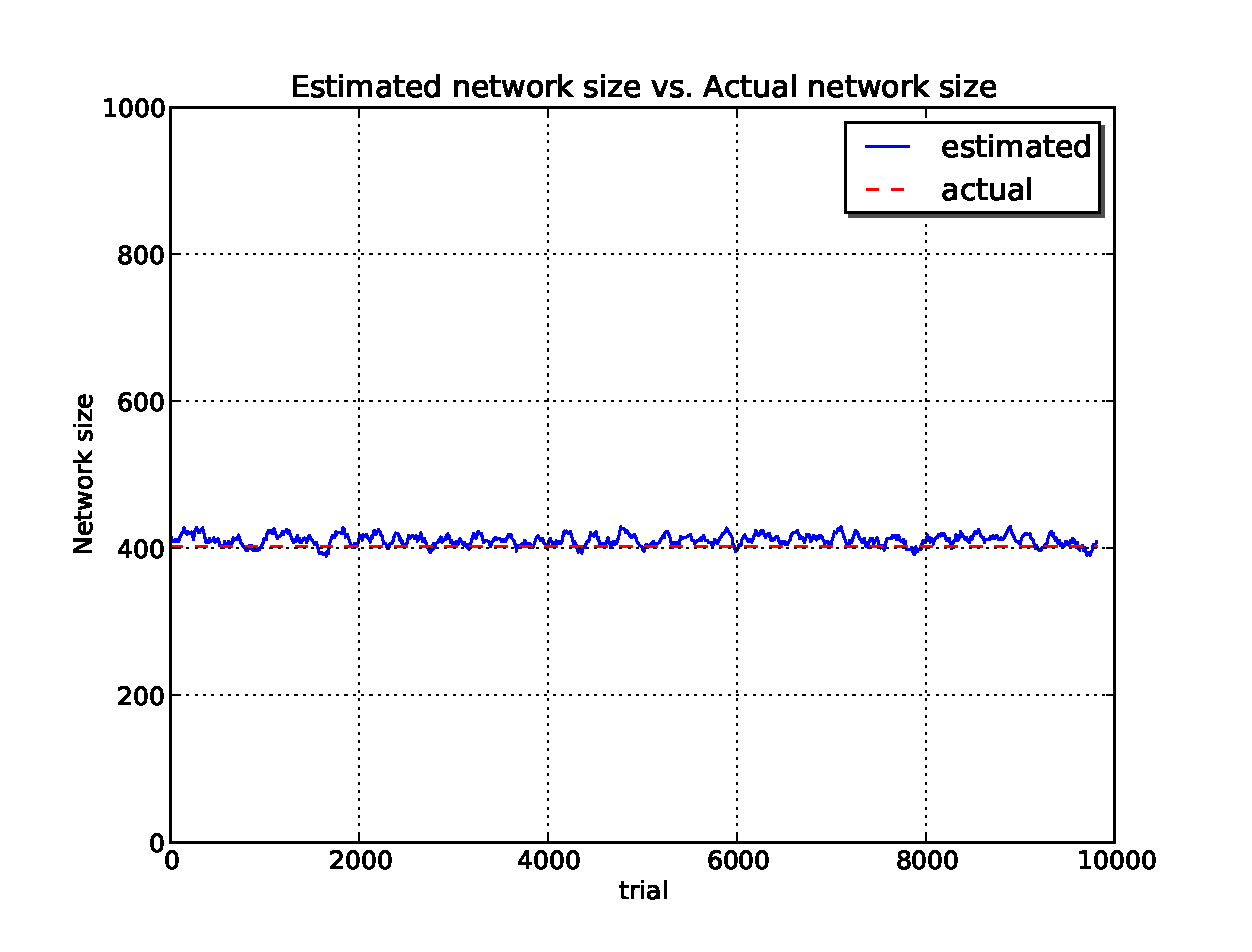
\includegraphics[scale=0.4]{figs/plab_size.eps}
\end{center}
\end{frame}


%%%%%%%%% SLIDE %%%%%%%%%%%%%%%%
%\begin{frame}
%\frametitle{Leave, Merge, Stabilization}
%\begin{itemize}
%\item Leave
%\item Merge
%\item Stabilization
%\end{itemize}
%\end{frame}

%%%%%%%%% SLIDE %%%%%%%%%%%%%%%%
\begin{frame}
\frametitle{}
\begin{itemize}
\item 
\item 
\end{itemize}
\end{frame}

%%%%%%%%% SLIDE %%%%%%%%%%%%%%%%
\begin{frame}
\frametitle{}
\begin{itemize}
\item 
\item 
\end{itemize}
\end{frame}

%%%%%%%%% SLIDE %%%%%%%%%%%%%%%%
\begin{frame}
\frametitle{Results:}
\begin{itemize}
\item 
\item 
\end{itemize}
\end{frame}

%%%%%%%%% SLIDE %%%%%%%%%%%%%%%%
\begin{frame}
\frametitle{Results:}
\begin{itemize}
\item 
\end{itemize}
\begin{center}
\includegraphics[]{figs/}
\end{center}
\end{frame}

%%%%%%%%% SLIDE %%%%%%%%%%%%%%%%
\begin{frame}
\frametitle{Contribution}
\begin{itemize}
\item 
\item 
\end{itemize}
\end{frame}

%~~~~~~~~~~~~~~~~~~~~~~~~~~~~~~~~~~~~~~~~~~~~~~~~~~~~~~%
%%%%%%%%% SLIDE %%%%%%%%%%%%%%%%
\section{Conclusion}
\frame<beamer>{\tableofcontents[current]}
\begin{frame}
\frametitle{Conclusion}
\begin{itemize}
\item Idea of modulization of reusable P2P algorithm 
\item Network size estimator
\item Search engine
\item Search engine for P2P DB
\end{itemize}
\end{frame}


%%%%%%%%% SLIDE %%%%%%%%%%%%%%%%

\begin{frame}
\begin{center}
\centering                        \huge Questions?
\end{center}
\end{frame}

 
\end{document}
